\documentclass{book}

\usepackage[dvipsnames]{xcolor}
\usepackage[most]{tcolorbox}
\usepackage[format=plain, labelfont=it, textfont=it]{caption}
\usepackage{amssymb}
\usepackage{amsfonts}
\usepackage{amsmath}
\usepackage{graphicx}
\usepackage{units}
\usepackage{hyperref}
\usepackage{listings}
\usepackage{pythonhighlight}
%\usepackage{authblk}

\graphicspath {{Figures/}}

 %%%%%%%%%%%%%%%%%%%%%%%%%%%%%%%%%%%%%%%%%%%%%%%%%%%%%%%%%%%%%%%%%%%%%%%%%%%%%%%% 
%%% ~ Arduino Language - Arduino IDE Colors ~                                  %%%
%%%                                                                            %%%
%%% Kyle Rocha-Brownell | 10/2/2017 | No Licence                               %%%
%%% -------------------------------------------------------------------------- %%%
%%%                                                                            %%%
%%% Place this file in your working directory (next to the latex file you're   %%%
%%% working on).  To add it to your project, place:                            %%%
%%%     %%%%%%%%%%%%%%%%%%%%%%%%%%%%%%%%%%%%%%%%%%%%%%%%%%%%%%%%%%%%%%%%%%%%%%%%%%%%%%%% 
%%% ~ Arduino Language - Arduino IDE Colors ~                                  %%%
%%%                                                                            %%%
%%% Kyle Rocha-Brownell | 10/2/2017 | No Licence                               %%%
%%% -------------------------------------------------------------------------- %%%
%%%                                                                            %%%
%%% Place this file in your working directory (next to the latex file you're   %%%
%%% working on).  To add it to your project, place:                            %%%
%%%     %%%%%%%%%%%%%%%%%%%%%%%%%%%%%%%%%%%%%%%%%%%%%%%%%%%%%%%%%%%%%%%%%%%%%%%%%%%%%%%% 
%%% ~ Arduino Language - Arduino IDE Colors ~                                  %%%
%%%                                                                            %%%
%%% Kyle Rocha-Brownell | 10/2/2017 | No Licence                               %%%
%%% -------------------------------------------------------------------------- %%%
%%%                                                                            %%%
%%% Place this file in your working directory (next to the latex file you're   %%%
%%% working on).  To add it to your project, place:                            %%%
%%%    \input{arduinoLanguage.tex}                                             %%%
%%% somewhere before \begin{document} in your latex file.                      %%%
%%%                                                                            %%%
%%% In your document, place your arduino code between:                         %%%
%%%   \begin{lstlisting}[language=Arduino]                                     %%%
%%% and:                                                                       %%%
%%%   \end{lstlisting}                                                         %%%
%%%                                                                            %%%
%%% Or create your own style to add non-built-in functions and variables.      %%%
%%%                                                                            %%%
 %%%%%%%%%%%%%%%%%%%%%%%%%%%%%%%%%%%%%%%%%%%%%%%%%%%%%%%%%%%%%%%%%%%%%%%%%%%%%%%% 

\usepackage{color}
\usepackage{listings}    
\usepackage{courier}

%%% Define Custom IDE Colors %%%
\definecolor{arduinoGreen}    {rgb} {0.17, 0.43, 0.01}
\definecolor{arduinoGrey}     {rgb} {0.47, 0.47, 0.33}
\definecolor{arduinoOrange}   {rgb} {0.8 , 0.4 , 0   }
\definecolor{arduinoBlue}     {rgb} {0.01, 0.61, 0.98}
\definecolor{arduinoDarkBlue} {rgb} {0.0 , 0.2 , 0.5 }

%%% Define Arduino Language %%%
\lstdefinelanguage{Arduino}{
  language=C++, % begin with default C++ settings 
%
%
  %%% Keyword Color Group 1 %%%  (called KEYWORD3 by arduino)
  keywordstyle=\color{arduinoGreen},   
  deletekeywords={  % remove all arduino keywords that might be in c++
                break, case, override, final, continue, default, do, else, for, 
                if, return, goto, switch, throw, try, while, setup, loop, export, 
                not, or, and, xor, include, define, elif, else, error, if, ifdef, 
                ifndef, pragma, warning,
                HIGH, LOW, INPUT, INPUT_PULLUP, OUTPUT, DEC, BIN, HEX, OCT, PI, 
                HALF_PI, TWO_PI, LSBFIRST, MSBFIRST, CHANGE, FALLING, RISING, 
                DEFAULT, EXTERNAL, INTERNAL, INTERNAL1V1, INTERNAL2V56, LED_BUILTIN, 
                LED_BUILTIN_RX, LED_BUILTIN_TX, DIGITAL_MESSAGE, FIRMATA_STRING, 
                ANALOG_MESSAGE, REPORT_DIGITAL, REPORT_ANALOG, SET_PIN_MODE, 
                SYSTEM_RESET, SYSEX_START, auto, int8_t, int16_t, int32_t, int64_t, 
                uint8_t, uint16_t, uint32_t, uint64_t, char16_t, char32_t, operator, 
                enum, delete, bool, boolean, byte, char, const, false, float, double, 
                null, NULL, int, long, new, private, protected, public, short, 
                signed, static, volatile, String, void, true, unsigned, word, array, 
                sizeof, dynamic_cast, typedef, const_cast, struct, static_cast, union, 
                friend, extern, class, reinterpret_cast, register, explicit, inline, 
                _Bool, complex, _Complex, _Imaginary, atomic_bool, atomic_char, 
                atomic_schar, atomic_uchar, atomic_short, atomic_ushort, atomic_int, 
                atomic_uint, atomic_long, atomic_ulong, atomic_llong, atomic_ullong, 
                virtual, PROGMEM,
                Serial, Serial1, Serial2, Serial3, SerialUSB, Keyboard, Mouse,
                abs, acos, asin, atan, atan2, ceil, constrain, cos, degrees, exp, 
                floor, log, map, max, min, radians, random, randomSeed, round, sin, 
                sq, sqrt, tan, pow, bitRead, bitWrite, bitSet, bitClear, bit, 
                highByte, lowByte, analogReference, analogRead, 
                analogReadResolution, analogWrite, analogWriteResolution, 
                attachInterrupt, detachInterrupt, digitalPinToInterrupt, delay, 
                delayMicroseconds, digitalWrite, digitalRead, interrupts, millis, 
                micros, noInterrupts, noTone, pinMode, pulseIn, pulseInLong, shiftIn, 
                shiftOut, tone, yield, Stream, begin, end, peek, read, print, 
                println, available, availableForWrite, flush, setTimeout, find, 
                findUntil, parseInt, parseFloat, readBytes, readBytesUntil, readString, 
                readStringUntil, trim, toUpperCase, toLowerCase, charAt, compareTo, 
                concat, endsWith, startsWith, equals, equalsIgnoreCase, getBytes, 
                indexOf, lastIndexOf, length, replace, setCharAt, substring, 
                toCharArray, toInt, press, release, releaseAll, accept, click, move, 
                isPressed, isAlphaNumeric, isAlpha, isAscii, isWhitespace, isControl, 
                isDigit, isGraph, isLowerCase, isPrintable, isPunct, isSpace, 
                isUpperCase, isHexadecimalDigit, 
                }, 
  morekeywords={   % add arduino structures to group 1
                break, case, override, final, continue, default, do, else, for, 
                if, return, goto, switch, throw, try, while, setup, loop, export, 
                not, or, and, xor, include, define, elif, else, error, if, ifdef, 
                ifndef, pragma, warning,
                }, 
% 
%
  %%% Keyword Color Group 2 %%%  (called LITERAL1 by arduino)
  keywordstyle=[2]\color{arduinoBlue},   
  keywords=[2]{   % add variables and dataTypes as 2nd group  
                HIGH, LOW, INPUT, INPUT_PULLUP, OUTPUT, DEC, BIN, HEX, OCT, PI, 
                HALF_PI, TWO_PI, LSBFIRST, MSBFIRST, CHANGE, FALLING, RISING, 
                DEFAULT, EXTERNAL, INTERNAL, INTERNAL1V1, INTERNAL2V56, LED_BUILTIN, 
                LED_BUILTIN_RX, LED_BUILTIN_TX, DIGITAL_MESSAGE, FIRMATA_STRING, 
                ANALOG_MESSAGE, REPORT_DIGITAL, REPORT_ANALOG, SET_PIN_MODE, 
                SYSTEM_RESET, SYSEX_START, auto, int8_t, int16_t, int32_t, int64_t, 
                uint8_t, uint16_t, uint32_t, uint64_t, char16_t, char32_t, operator, 
                enum, delete, bool, boolean, byte, char, const, false, float, double, 
                null, NULL, int, long, new, private, protected, public, short, 
                signed, static, volatile, String, void, true, unsigned, word, array, 
                sizeof, dynamic_cast, typedef, const_cast, struct, static_cast, union, 
                friend, extern, class, reinterpret_cast, register, explicit, inline, 
                _Bool, complex, _Complex, _Imaginary, atomic_bool, atomic_char, 
                atomic_schar, atomic_uchar, atomic_short, atomic_ushort, atomic_int, 
                atomic_uint, atomic_long, atomic_ulong, atomic_llong, atomic_ullong, 
                virtual, PROGMEM,
                },  
% 
%
  %%% Keyword Color Group 3 %%%  (called KEYWORD1 by arduino)
  keywordstyle=[3]\bfseries\color{arduinoOrange},
  keywords=[3]{  % add built-in functions as a 3rd group
                Serial, Serial1, Serial2, Serial3, SerialUSB, Keyboard, Mouse,
                },      
%
%
  %%% Keyword Color Group 4 %%%  (called KEYWORD2 by arduino)
  keywordstyle=[4]\color{arduinoOrange},
  keywords=[4]{  % add more built-in functions as a 4th group
                abs, acos, asin, atan, atan2, ceil, constrain, cos, degrees, exp, 
                floor, log, map, max, min, radians, random, randomSeed, round, sin, 
                sq, sqrt, tan, pow, bitRead, bitWrite, bitSet, bitClear, bit, 
                highByte, lowByte, analogReference, analogRead, 
                analogReadResolution, analogWrite, analogWriteResolution, 
                attachInterrupt, detachInterrupt, digitalPinToInterrupt, delay, 
                delayMicroseconds, digitalWrite, digitalRead, interrupts, millis, 
                micros, noInterrupts, noTone, pinMode, pulseIn, pulseInLong, shiftIn, 
                shiftOut, tone, yield, Stream, begin, end, peek, read, print, 
                println, available, availableForWrite, flush, setTimeout, find, 
                findUntil, parseInt, parseFloat, readBytes, readBytesUntil, readString, 
                readStringUntil, trim, toUpperCase, toLowerCase, charAt, compareTo, 
                concat, endsWith, startsWith, equals, equalsIgnoreCase, getBytes, 
                indexOf, lastIndexOf, length, replace, setCharAt, substring, 
                toCharArray, toInt, press, release, releaseAll, accept, click, move, 
                isPressed, isAlphaNumeric, isAlpha, isAscii, isWhitespace, isControl, 
                isDigit, isGraph, isLowerCase, isPrintable, isPunct, isSpace, 
                isUpperCase, isHexadecimalDigit, 
                },      
%
%
  %%% Set Other Colors %%%
  stringstyle=\color{arduinoDarkBlue},    
  commentstyle=\color{arduinoGrey},    
%          
%   
  %%%% Line Numbering %%%%
%  numbers=left,                    
%  numbersep=5pt,                   
%  numberstyle=\color{arduinoGrey},    
  %stepnumber=2,                      % show every 2 line numbers
%
%
  frame=single, 	% Adds a boxed frame around the code
  %%%% Code Box Style %%%%
  breaklines=false,%true,                    % wordwrapping
  tabsize=2,         
  basicstyle=\ttfamily
}
                                             %%%
%%% somewhere before \begin{document} in your latex file.                      %%%
%%%                                                                            %%%
%%% In your document, place your arduino code between:                         %%%
%%%   \begin{lstlisting}[language=Arduino]                                     %%%
%%% and:                                                                       %%%
%%%   \end{lstlisting}                                                         %%%
%%%                                                                            %%%
%%% Or create your own style to add non-built-in functions and variables.      %%%
%%%                                                                            %%%
 %%%%%%%%%%%%%%%%%%%%%%%%%%%%%%%%%%%%%%%%%%%%%%%%%%%%%%%%%%%%%%%%%%%%%%%%%%%%%%%% 

\usepackage{color}
\usepackage{listings}    
\usepackage{courier}

%%% Define Custom IDE Colors %%%
\definecolor{arduinoGreen}    {rgb} {0.17, 0.43, 0.01}
\definecolor{arduinoGrey}     {rgb} {0.47, 0.47, 0.33}
\definecolor{arduinoOrange}   {rgb} {0.8 , 0.4 , 0   }
\definecolor{arduinoBlue}     {rgb} {0.01, 0.61, 0.98}
\definecolor{arduinoDarkBlue} {rgb} {0.0 , 0.2 , 0.5 }

%%% Define Arduino Language %%%
\lstdefinelanguage{Arduino}{
  language=C++, % begin with default C++ settings 
%
%
  %%% Keyword Color Group 1 %%%  (called KEYWORD3 by arduino)
  keywordstyle=\color{arduinoGreen},   
  deletekeywords={  % remove all arduino keywords that might be in c++
                break, case, override, final, continue, default, do, else, for, 
                if, return, goto, switch, throw, try, while, setup, loop, export, 
                not, or, and, xor, include, define, elif, else, error, if, ifdef, 
                ifndef, pragma, warning,
                HIGH, LOW, INPUT, INPUT_PULLUP, OUTPUT, DEC, BIN, HEX, OCT, PI, 
                HALF_PI, TWO_PI, LSBFIRST, MSBFIRST, CHANGE, FALLING, RISING, 
                DEFAULT, EXTERNAL, INTERNAL, INTERNAL1V1, INTERNAL2V56, LED_BUILTIN, 
                LED_BUILTIN_RX, LED_BUILTIN_TX, DIGITAL_MESSAGE, FIRMATA_STRING, 
                ANALOG_MESSAGE, REPORT_DIGITAL, REPORT_ANALOG, SET_PIN_MODE, 
                SYSTEM_RESET, SYSEX_START, auto, int8_t, int16_t, int32_t, int64_t, 
                uint8_t, uint16_t, uint32_t, uint64_t, char16_t, char32_t, operator, 
                enum, delete, bool, boolean, byte, char, const, false, float, double, 
                null, NULL, int, long, new, private, protected, public, short, 
                signed, static, volatile, String, void, true, unsigned, word, array, 
                sizeof, dynamic_cast, typedef, const_cast, struct, static_cast, union, 
                friend, extern, class, reinterpret_cast, register, explicit, inline, 
                _Bool, complex, _Complex, _Imaginary, atomic_bool, atomic_char, 
                atomic_schar, atomic_uchar, atomic_short, atomic_ushort, atomic_int, 
                atomic_uint, atomic_long, atomic_ulong, atomic_llong, atomic_ullong, 
                virtual, PROGMEM,
                Serial, Serial1, Serial2, Serial3, SerialUSB, Keyboard, Mouse,
                abs, acos, asin, atan, atan2, ceil, constrain, cos, degrees, exp, 
                floor, log, map, max, min, radians, random, randomSeed, round, sin, 
                sq, sqrt, tan, pow, bitRead, bitWrite, bitSet, bitClear, bit, 
                highByte, lowByte, analogReference, analogRead, 
                analogReadResolution, analogWrite, analogWriteResolution, 
                attachInterrupt, detachInterrupt, digitalPinToInterrupt, delay, 
                delayMicroseconds, digitalWrite, digitalRead, interrupts, millis, 
                micros, noInterrupts, noTone, pinMode, pulseIn, pulseInLong, shiftIn, 
                shiftOut, tone, yield, Stream, begin, end, peek, read, print, 
                println, available, availableForWrite, flush, setTimeout, find, 
                findUntil, parseInt, parseFloat, readBytes, readBytesUntil, readString, 
                readStringUntil, trim, toUpperCase, toLowerCase, charAt, compareTo, 
                concat, endsWith, startsWith, equals, equalsIgnoreCase, getBytes, 
                indexOf, lastIndexOf, length, replace, setCharAt, substring, 
                toCharArray, toInt, press, release, releaseAll, accept, click, move, 
                isPressed, isAlphaNumeric, isAlpha, isAscii, isWhitespace, isControl, 
                isDigit, isGraph, isLowerCase, isPrintable, isPunct, isSpace, 
                isUpperCase, isHexadecimalDigit, 
                }, 
  morekeywords={   % add arduino structures to group 1
                break, case, override, final, continue, default, do, else, for, 
                if, return, goto, switch, throw, try, while, setup, loop, export, 
                not, or, and, xor, include, define, elif, else, error, if, ifdef, 
                ifndef, pragma, warning,
                }, 
% 
%
  %%% Keyword Color Group 2 %%%  (called LITERAL1 by arduino)
  keywordstyle=[2]\color{arduinoBlue},   
  keywords=[2]{   % add variables and dataTypes as 2nd group  
                HIGH, LOW, INPUT, INPUT_PULLUP, OUTPUT, DEC, BIN, HEX, OCT, PI, 
                HALF_PI, TWO_PI, LSBFIRST, MSBFIRST, CHANGE, FALLING, RISING, 
                DEFAULT, EXTERNAL, INTERNAL, INTERNAL1V1, INTERNAL2V56, LED_BUILTIN, 
                LED_BUILTIN_RX, LED_BUILTIN_TX, DIGITAL_MESSAGE, FIRMATA_STRING, 
                ANALOG_MESSAGE, REPORT_DIGITAL, REPORT_ANALOG, SET_PIN_MODE, 
                SYSTEM_RESET, SYSEX_START, auto, int8_t, int16_t, int32_t, int64_t, 
                uint8_t, uint16_t, uint32_t, uint64_t, char16_t, char32_t, operator, 
                enum, delete, bool, boolean, byte, char, const, false, float, double, 
                null, NULL, int, long, new, private, protected, public, short, 
                signed, static, volatile, String, void, true, unsigned, word, array, 
                sizeof, dynamic_cast, typedef, const_cast, struct, static_cast, union, 
                friend, extern, class, reinterpret_cast, register, explicit, inline, 
                _Bool, complex, _Complex, _Imaginary, atomic_bool, atomic_char, 
                atomic_schar, atomic_uchar, atomic_short, atomic_ushort, atomic_int, 
                atomic_uint, atomic_long, atomic_ulong, atomic_llong, atomic_ullong, 
                virtual, PROGMEM,
                },  
% 
%
  %%% Keyword Color Group 3 %%%  (called KEYWORD1 by arduino)
  keywordstyle=[3]\bfseries\color{arduinoOrange},
  keywords=[3]{  % add built-in functions as a 3rd group
                Serial, Serial1, Serial2, Serial3, SerialUSB, Keyboard, Mouse,
                },      
%
%
  %%% Keyword Color Group 4 %%%  (called KEYWORD2 by arduino)
  keywordstyle=[4]\color{arduinoOrange},
  keywords=[4]{  % add more built-in functions as a 4th group
                abs, acos, asin, atan, atan2, ceil, constrain, cos, degrees, exp, 
                floor, log, map, max, min, radians, random, randomSeed, round, sin, 
                sq, sqrt, tan, pow, bitRead, bitWrite, bitSet, bitClear, bit, 
                highByte, lowByte, analogReference, analogRead, 
                analogReadResolution, analogWrite, analogWriteResolution, 
                attachInterrupt, detachInterrupt, digitalPinToInterrupt, delay, 
                delayMicroseconds, digitalWrite, digitalRead, interrupts, millis, 
                micros, noInterrupts, noTone, pinMode, pulseIn, pulseInLong, shiftIn, 
                shiftOut, tone, yield, Stream, begin, end, peek, read, print, 
                println, available, availableForWrite, flush, setTimeout, find, 
                findUntil, parseInt, parseFloat, readBytes, readBytesUntil, readString, 
                readStringUntil, trim, toUpperCase, toLowerCase, charAt, compareTo, 
                concat, endsWith, startsWith, equals, equalsIgnoreCase, getBytes, 
                indexOf, lastIndexOf, length, replace, setCharAt, substring, 
                toCharArray, toInt, press, release, releaseAll, accept, click, move, 
                isPressed, isAlphaNumeric, isAlpha, isAscii, isWhitespace, isControl, 
                isDigit, isGraph, isLowerCase, isPrintable, isPunct, isSpace, 
                isUpperCase, isHexadecimalDigit, 
                },      
%
%
  %%% Set Other Colors %%%
  stringstyle=\color{arduinoDarkBlue},    
  commentstyle=\color{arduinoGrey},    
%          
%   
  %%%% Line Numbering %%%%
%  numbers=left,                    
%  numbersep=5pt,                   
%  numberstyle=\color{arduinoGrey},    
  %stepnumber=2,                      % show every 2 line numbers
%
%
  frame=single, 	% Adds a boxed frame around the code
  %%%% Code Box Style %%%%
  breaklines=false,%true,                    % wordwrapping
  tabsize=2,         
  basicstyle=\ttfamily
}
                                             %%%
%%% somewhere before \begin{document} in your latex file.                      %%%
%%%                                                                            %%%
%%% In your document, place your arduino code between:                         %%%
%%%   \begin{lstlisting}[language=Arduino]                                     %%%
%%% and:                                                                       %%%
%%%   \end{lstlisting}                                                         %%%
%%%                                                                            %%%
%%% Or create your own style to add non-built-in functions and variables.      %%%
%%%                                                                            %%%
 %%%%%%%%%%%%%%%%%%%%%%%%%%%%%%%%%%%%%%%%%%%%%%%%%%%%%%%%%%%%%%%%%%%%%%%%%%%%%%%% 

\usepackage{color}
\usepackage{listings}    
\usepackage{courier}

%%% Define Custom IDE Colors %%%
\definecolor{arduinoGreen}    {rgb} {0.17, 0.43, 0.01}
\definecolor{arduinoGrey}     {rgb} {0.47, 0.47, 0.33}
\definecolor{arduinoOrange}   {rgb} {0.8 , 0.4 , 0   }
\definecolor{arduinoBlue}     {rgb} {0.01, 0.61, 0.98}
\definecolor{arduinoDarkBlue} {rgb} {0.0 , 0.2 , 0.5 }

%%% Define Arduino Language %%%
\lstdefinelanguage{Arduino}{
  language=C++, % begin with default C++ settings 
%
%
  %%% Keyword Color Group 1 %%%  (called KEYWORD3 by arduino)
  keywordstyle=\color{arduinoGreen},   
  deletekeywords={  % remove all arduino keywords that might be in c++
                break, case, override, final, continue, default, do, else, for, 
                if, return, goto, switch, throw, try, while, setup, loop, export, 
                not, or, and, xor, include, define, elif, else, error, if, ifdef, 
                ifndef, pragma, warning,
                HIGH, LOW, INPUT, INPUT_PULLUP, OUTPUT, DEC, BIN, HEX, OCT, PI, 
                HALF_PI, TWO_PI, LSBFIRST, MSBFIRST, CHANGE, FALLING, RISING, 
                DEFAULT, EXTERNAL, INTERNAL, INTERNAL1V1, INTERNAL2V56, LED_BUILTIN, 
                LED_BUILTIN_RX, LED_BUILTIN_TX, DIGITAL_MESSAGE, FIRMATA_STRING, 
                ANALOG_MESSAGE, REPORT_DIGITAL, REPORT_ANALOG, SET_PIN_MODE, 
                SYSTEM_RESET, SYSEX_START, auto, int8_t, int16_t, int32_t, int64_t, 
                uint8_t, uint16_t, uint32_t, uint64_t, char16_t, char32_t, operator, 
                enum, delete, bool, boolean, byte, char, const, false, float, double, 
                null, NULL, int, long, new, private, protected, public, short, 
                signed, static, volatile, String, void, true, unsigned, word, array, 
                sizeof, dynamic_cast, typedef, const_cast, struct, static_cast, union, 
                friend, extern, class, reinterpret_cast, register, explicit, inline, 
                _Bool, complex, _Complex, _Imaginary, atomic_bool, atomic_char, 
                atomic_schar, atomic_uchar, atomic_short, atomic_ushort, atomic_int, 
                atomic_uint, atomic_long, atomic_ulong, atomic_llong, atomic_ullong, 
                virtual, PROGMEM,
                Serial, Serial1, Serial2, Serial3, SerialUSB, Keyboard, Mouse,
                abs, acos, asin, atan, atan2, ceil, constrain, cos, degrees, exp, 
                floor, log, map, max, min, radians, random, randomSeed, round, sin, 
                sq, sqrt, tan, pow, bitRead, bitWrite, bitSet, bitClear, bit, 
                highByte, lowByte, analogReference, analogRead, 
                analogReadResolution, analogWrite, analogWriteResolution, 
                attachInterrupt, detachInterrupt, digitalPinToInterrupt, delay, 
                delayMicroseconds, digitalWrite, digitalRead, interrupts, millis, 
                micros, noInterrupts, noTone, pinMode, pulseIn, pulseInLong, shiftIn, 
                shiftOut, tone, yield, Stream, begin, end, peek, read, print, 
                println, available, availableForWrite, flush, setTimeout, find, 
                findUntil, parseInt, parseFloat, readBytes, readBytesUntil, readString, 
                readStringUntil, trim, toUpperCase, toLowerCase, charAt, compareTo, 
                concat, endsWith, startsWith, equals, equalsIgnoreCase, getBytes, 
                indexOf, lastIndexOf, length, replace, setCharAt, substring, 
                toCharArray, toInt, press, release, releaseAll, accept, click, move, 
                isPressed, isAlphaNumeric, isAlpha, isAscii, isWhitespace, isControl, 
                isDigit, isGraph, isLowerCase, isPrintable, isPunct, isSpace, 
                isUpperCase, isHexadecimalDigit, 
                }, 
  morekeywords={   % add arduino structures to group 1
                break, case, override, final, continue, default, do, else, for, 
                if, return, goto, switch, throw, try, while, setup, loop, export, 
                not, or, and, xor, include, define, elif, else, error, if, ifdef, 
                ifndef, pragma, warning,
                }, 
% 
%
  %%% Keyword Color Group 2 %%%  (called LITERAL1 by arduino)
  keywordstyle=[2]\color{arduinoBlue},   
  keywords=[2]{   % add variables and dataTypes as 2nd group  
                HIGH, LOW, INPUT, INPUT_PULLUP, OUTPUT, DEC, BIN, HEX, OCT, PI, 
                HALF_PI, TWO_PI, LSBFIRST, MSBFIRST, CHANGE, FALLING, RISING, 
                DEFAULT, EXTERNAL, INTERNAL, INTERNAL1V1, INTERNAL2V56, LED_BUILTIN, 
                LED_BUILTIN_RX, LED_BUILTIN_TX, DIGITAL_MESSAGE, FIRMATA_STRING, 
                ANALOG_MESSAGE, REPORT_DIGITAL, REPORT_ANALOG, SET_PIN_MODE, 
                SYSTEM_RESET, SYSEX_START, auto, int8_t, int16_t, int32_t, int64_t, 
                uint8_t, uint16_t, uint32_t, uint64_t, char16_t, char32_t, operator, 
                enum, delete, bool, boolean, byte, char, const, false, float, double, 
                null, NULL, int, long, new, private, protected, public, short, 
                signed, static, volatile, String, void, true, unsigned, word, array, 
                sizeof, dynamic_cast, typedef, const_cast, struct, static_cast, union, 
                friend, extern, class, reinterpret_cast, register, explicit, inline, 
                _Bool, complex, _Complex, _Imaginary, atomic_bool, atomic_char, 
                atomic_schar, atomic_uchar, atomic_short, atomic_ushort, atomic_int, 
                atomic_uint, atomic_long, atomic_ulong, atomic_llong, atomic_ullong, 
                virtual, PROGMEM,
                },  
% 
%
  %%% Keyword Color Group 3 %%%  (called KEYWORD1 by arduino)
  keywordstyle=[3]\bfseries\color{arduinoOrange},
  keywords=[3]{  % add built-in functions as a 3rd group
                Serial, Serial1, Serial2, Serial3, SerialUSB, Keyboard, Mouse,
                },      
%
%
  %%% Keyword Color Group 4 %%%  (called KEYWORD2 by arduino)
  keywordstyle=[4]\color{arduinoOrange},
  keywords=[4]{  % add more built-in functions as a 4th group
                abs, acos, asin, atan, atan2, ceil, constrain, cos, degrees, exp, 
                floor, log, map, max, min, radians, random, randomSeed, round, sin, 
                sq, sqrt, tan, pow, bitRead, bitWrite, bitSet, bitClear, bit, 
                highByte, lowByte, analogReference, analogRead, 
                analogReadResolution, analogWrite, analogWriteResolution, 
                attachInterrupt, detachInterrupt, digitalPinToInterrupt, delay, 
                delayMicroseconds, digitalWrite, digitalRead, interrupts, millis, 
                micros, noInterrupts, noTone, pinMode, pulseIn, pulseInLong, shiftIn, 
                shiftOut, tone, yield, Stream, begin, end, peek, read, print, 
                println, available, availableForWrite, flush, setTimeout, find, 
                findUntil, parseInt, parseFloat, readBytes, readBytesUntil, readString, 
                readStringUntil, trim, toUpperCase, toLowerCase, charAt, compareTo, 
                concat, endsWith, startsWith, equals, equalsIgnoreCase, getBytes, 
                indexOf, lastIndexOf, length, replace, setCharAt, substring, 
                toCharArray, toInt, press, release, releaseAll, accept, click, move, 
                isPressed, isAlphaNumeric, isAlpha, isAscii, isWhitespace, isControl, 
                isDigit, isGraph, isLowerCase, isPrintable, isPunct, isSpace, 
                isUpperCase, isHexadecimalDigit, 
                },      
%
%
  %%% Set Other Colors %%%
  stringstyle=\color{arduinoDarkBlue},    
  commentstyle=\color{arduinoGrey},    
%          
%   
  %%%% Line Numbering %%%%
%  numbers=left,                    
%  numbersep=5pt,                   
%  numberstyle=\color{arduinoGrey},    
  %stepnumber=2,                      % show every 2 line numbers
%
%
  frame=single, 	% Adds a boxed frame around the code
  %%%% Code Box Style %%%%
  breaklines=false,%true,                    % wordwrapping
  tabsize=2,         
  basicstyle=\ttfamily
}
 % provies color formating for the Arduino Language. It loads and uses the \usepackage{listings}  
% Macros used in the textbook (avoids rewriting a bunch of LaTeX markup...

\newcommand{\objectives}[1]
{
  \begin{center}
  \setlength{\fboxsep}{15pt}
  \fcolorbox{Black}{Apricot}
  {
    \begin{minipage}{0.80\textwidth}
    \begin{center}
    \textbf{OBJECTIVES}
    \end{center}
    \begin{itemize} #1 \end{itemize}
    \end{minipage}
  }
  \end{center}
}

\newcommand{\review}[1]
{
  \begin{center}
  \setlength{\fboxsep}{15pt}
  \fcolorbox{Black}{Aquamarine}
  {
    \begin{minipage}{0.80\textwidth}
    \begin{center}
    \textbf{ITEMS TO REVIEW}
    \end{center}
    Please review the following concepts in your electricity and magnetism
    textbook.
    \begin{itemize} #1 \end{itemize}
    \end{minipage}
  }
  \end{center}
}

\newcommand{\warning}[1]
{
  \begin{center}
  \setlength{\fboxsep}{10pt}
  \fcolorbox{Black}{Red}
  {
%    \begin{minipage}
    \fcolorbox{Black}{Yellow}
    {
      \begin{center}
      \color{Red}
      \textbf{WARNING}
      \end{center}
%      #1
    }
%    \end{minipage}
  }
  \end{center}
}

 % Provides the macros for the objectives and review boxes
% at the top of each chapter.


%\newenvironment{python}{\begin{lstlisting}[language=Python]}{\end{lstlisting}}


\begin{document}

\frontmatter
\title{{\Huge PH 250}\\
{\Huge {\Large Intermediate Physics Laboratory for Physics and Physical
Science Teaching Majors} }}
\author{R Todd Lines\\ David Oliphant\\ Kevin Kelley}

\date{\today}
\maketitle
\tableofcontents
\listoffigures

%\chapter*{Preface}
%Preface
\chapter*{Preface}
Experimental physics is the art of testing our physical models to see if they really work. Thousands of measuring devices have been designed and built to make the detailed measurements needed to perform this testing. We would like to interface these measuring devices to computers so data collection is all digital. Then the data can be analyzed, and displayed on our computers. To do this we need to understand computer interfacing.

Computer interfacing is a bit of engineering. We need to either design and build, or purchase instruments, and then get data from those instruments into a computer. But even though it is an engineering task, it is a necessary skill for experimental physicists. It is this skill that we wish to take on in this laboratory class. Of course we can't learn all that there is to know on computer interfacing in one semester. But we can make a good start.

We will use the open source Arduino microcontroler board as our computer interface and we will use Python and the Arduino C++ languages to write controlling software.

Students should leave this class with confidence that they can build a simple computer interface that will read in sensor data and save it on a computer.

Students in this class will also spend time investigating physical models from introductory electricity and magnetism theory.

Instrumentation is sometimes difficult, sometimes frustrating, but also a lot of fun. I hope you will find these lab experiences both informative and entertaining. 

I would like to acknowledge Tyler Miller who has spent countless hours testing the codes and writing the Mac versions and helping to improve the text. 



%\chapter{Introduction}
%Introduction
\chapter*{Introduction}
\addcontentsline{toc}{chapter}{\protect\numberline{}Introduction}

As a PH250 student, you are probably taking PH220 concurrently with PH250. This lab course is designed to teach electronics and computer skills while your PH220 professor teaches electromagnetic field theory. Once you have a little bit of electric field theory under your belt from PH220, then our experiments designed to test out models of electric charge and electromagnetic fields begin in earnest. While we are waiting we will spend some time learning about how to control experiments with a computer, and how to import data from an experiment to a computer.

You should read the material for each lab before the lab begins. There will sometimes be practice problems to do to make sure you will be effective in lab. By preparing before lab you will have the full 2 hours and 45 minutes to make sure you can finish the lab work. Some labs may go fast, but most take the entire lab period. I also suggest you practice your computer and electronics skills a little. Build some blinking lights for your apartment, or measure how loud your roommates are, or something. The Arduino can be the data collection and control part of thousands fun projects.

This class is sometimes frustrating. But it is also a lot of fun. You will be introduced to computer instrumentation and will be able to perform an experiment that you and your lab group design. The student designed experiments are only limited by your imagination and our ability to find equipment. If you have concerns during the semester, don't hesitate to find your instructor or TA and ask.

\section*{Keeping a Lab Notebook}
\addcontentsline{toc}{section}{\protect\numberline{}Keeping a Lab Notebook}

Keeping a detailed and accurate record is a critical laboratory skill. An 
informal version of this record is often referred to as a ``lab notebook'',
because traditionally they were kept in physical paper notebooks. Lab
notebooks would include written notes and observations, equations, and sketches
of the experimental apparatus. With the advent of modern technology, we can
make these lab notebook even better. If kept as an electronic document, you
can easily copy and paste code into the lab notebook, or include photographs
of your experiment.

One requirement of this course is that you submit a lab notebook for each
lab. The criteria on which they will be graded can be found on your course
syllabus or on the learning management system.

\section*{Using This Lab Manual}
\addcontentsline{toc}{section}{\protect\numberline{}Using This Lab Manual}

You should plan on reading the appropriate chapter of the lab manual before 
you come to each lab activity. This will save you a lot of time once you get
into the lab, as you'll already have the ``big picture'' of what we are doing,
and also kind of know how you should proceed. Trying to read along as you go
in lab will simply result in you still being in lab after everyone else has
finished and left.

Each chapter has a defined list of objectives that tell you what you should
be able to do after each lab activity. These objectives are found in a callout
box that appears as follows:
\objectives{
\item Objective no. 1....
\item Objective no. 2....
\item etc....
}

As you begin reading the chapter, pay attention to these objectives. When you
have completed the lab, ask yourself whether you have fulfilled those 
objectives (and whether you would be able to do so again).

Below the objectives, you will find another callout box identifying the 
concepts that you will need to know from your electricity and magnetism 
course. Rather than rehash all of those topics in this text, you should 
simply turn to your E\&M textbook (or another resource) and review any
items that are unfamiliar. The list of review items will appear as follows:
\review{
\item First topic to review....
\item Second topic to review....
\item etc....
}

As you proceed through the chapter, you will encounter places where you 
would now complete an activity in the lab. To make these activities easy to
find, they also can be found in callout boxes that look like the following:
\activity{
This is an example of an activity callout box. It will tell you what you need
to do at this point in the lab.}

% FIXME


\mainmatter

\part{Computer Interfacing}

	%\chapter{Introduction to the Arduino and Computer Control}
		%Intro_Arduino_ComputerControl
\chapter{Introduction to the Arduino}

\objectives{
\item Explain how to use a prototyping board, including the identification of
which pins are electrically connected.
\item Demostrate proper soldering technique.
\item Describe the two primary functions included in every Arduino sketch, when
they are called, and what they do.
\item Compile and upload sketches to an Arduino.
\item Demonstrate the use of digital output on the Arduino by constructing 
several circuits involving blinking lights.
}

\review{
\item Voltage (electric potential).
\item Current.
\item Resistance.
\item Diodes and LEDs.
}

There are two ways in which we want our computers to communicate with our
physics experiments:
\begin{enumerate}
\item Have the computer control the experiment. For example, we could have the
computer turn on our apparatus, or turn it off. 
\item Have the experimental device provide data to the computer. The computer
can then record this data for later analysis.
\end{enumerate}
In both cases, we need something that goes between the
experimental measuring devices and the computer. These go-between pieces are
often called Data Acquisition (DAQ) boards. There are many different forms
of DAQs. They can cost anywhere from a few dollars to many thousands of
dollars.

In this lab, we will use a low cost DAQ, the plans for which the 
developers placed in the open-source world so that no one
would get royalties (including themselves) for the design (this is why the
boards are inexpensive). It is low cost, but not low
quality. The developers named their DAQ the ``Arduino''. There are many
different variations on the Arduino. We will specifically be using the
Arduino UNO.

Like all DAQs, the Arduino is fragile, so we will need to exercise some 
caution. Arduinos can be destroyed by putting too large a voltage or electrical 
current into the input pins. They also can be destroyed by mechanical means, 
such as being dropped or crushed.

By the end of this chapter, you will have successfully used an Arduino to 
communicate with an electric circuit. However, before we can interface with
a circuit, we have to build one.

%%%%%%%%%%%%%%%%%%%%%%%%%%%%%%%%%%%%%%%%%%%%%%%%%%%%%%%%%%%%%%%%%%%%%%%%%%%%%%%%

\section{Building circuits}

When you are first designing and constructing a circuit, you want to be able to 
easily and quickly make and revise electrical connections. Once the circuit
is designed, you often want to make it more permanent with solid connections
that cannot be jostled loose. We'll now consider how we go about building these
temporary and longer lasting circuits.

\subsection{Temporary circuits: the prototyping board}

Temporary circuits are usually built on a prototyping board, which is a plastic
board full of holes, as seen in Figure \ref{fig:protoboard_blank}. Each of the
holes in the prototyping board (sometimes a called a ``protoboard'' or 
``breadboard'') is a place where you can insert the lead from an electrical 
component, such as a resistor or capacitor, or a wire. 
(A ``lead'' is one of the wires
protruding from the component.)
\begin{figure}[hbp!]
\centering
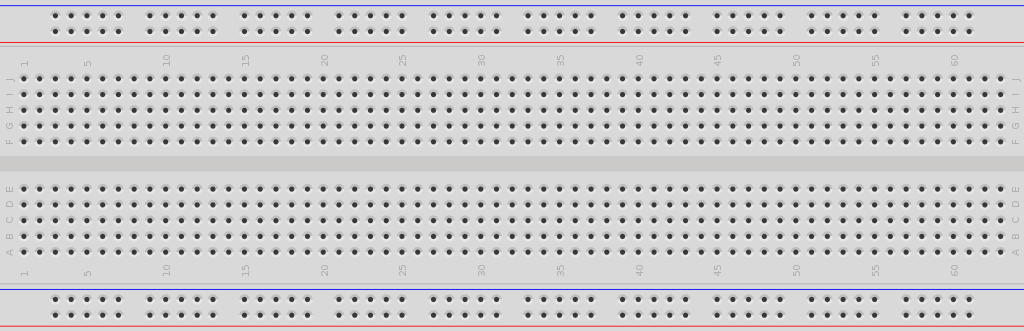
\includegraphics[width=0.8\textwidth]{protoboard_blank}
\caption[An empty prototyping board]{An empty prototyping board.}
\label{fig:protoboard_blank}
\end{figure}

The advantage of a prototyping board is that each of the holes is electrically 
connected to at least four other holes. Thus, by plugging leads wires 
into two connected holes, the leads or wires are now electrically 
connected to each other. The connections in a prototyping board are typically
as follows:
\begin{itemize}
\item All of the holes adjacent to each of the blue lines are connected. 
These are typically used for connections to an electrical ground or the
negative terminal of a power source.
\item All of the holes adjacent to each of the red lines are connected.
These are typically used for connections to an electrical power source 
(generally the positive terminal for DC power sources).
\item Each vertically oriented set of five holes in the center of the board
are connected.
\end{itemize}
These connections are illustrated in Figure \ref{fig:protoboard_connections}.
Please note that not all prototyping boards are alike, and the connections
may vary from board to board.
\begin{figure}[hbp!]
\centering
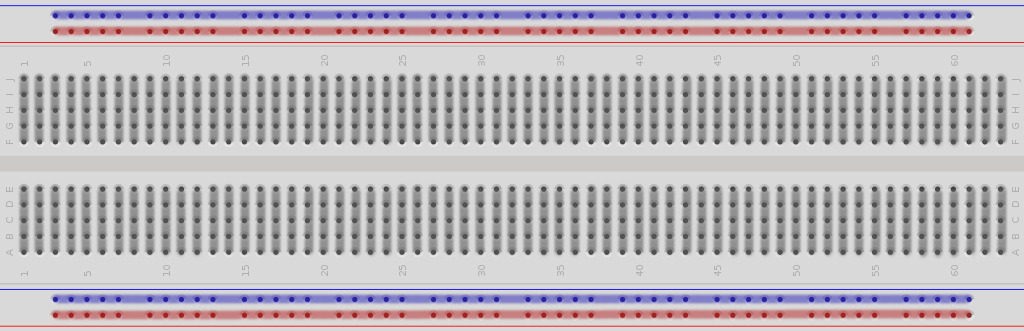
\includegraphics[width=0.8\textwidth]{protoboard_connections}
\caption[Typical connections on a prototyping board]{Typical connections on a
prototyping board. The holes adjacent to each of the red and blue lines are
connected to each other, as indicated by the red and blue highlights on
the figure. The remaining holes are connected in groups of five, as indicated
by the grey highlights.}
\label{fig:protoboard_connections}
\end{figure}

As an example, let's consider how we might wire together a simple circuit 
involving a 9 volt battery and an LED using a protyping board. Note that 
nine volts is usually a little high for powering a single LED, so we are also
going to put a resistor in our circuit to keep the current down.

First, let's connect our battery to the red an blue rows of the 
prototyping board. You don't necessarily have to connect the power this way 
(in fact, once you know how the connections in the prototyping board work, you
can connect things in any fashion consistent with the circuit you are trying 
to build), but doing so is generally considered good practice. We can also
connect each set of row together, so that we are providing a power 
source and ground at both the top and bottom of the board. As you know, the
color of the wires I use doesn't make any difference in how the circuit 
operates, but the colors \textit{can} help me keep track of how I've built my
circuit. Red is typically used for power sources, and dark blue or black is
typically used for ground (or the negative terminal for DC sources). Once I've
made these connections, my prototyping board looks like Figure
\ref{fig:protoboard_example_a}.
\begin{figure}[hbp!]
\centering
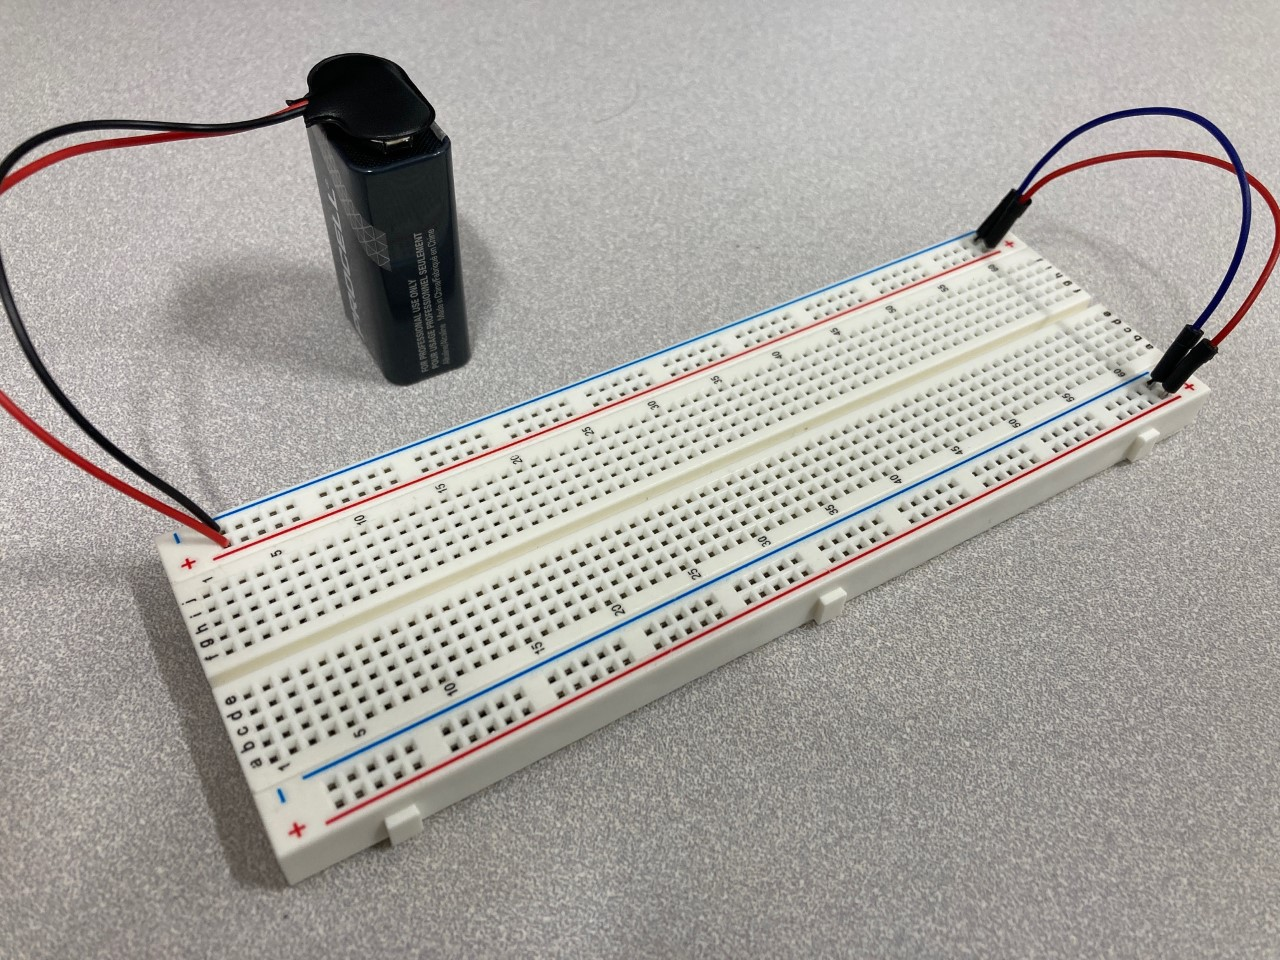
\includegraphics[width=0.8\textwidth]{protoboard_example_a}
\caption[Connecting power to a prototyping board]{Connecting power to a 
prototyping board. Note that the positive lead from the battery holder
connects to the ``red'' horizontal line on the prototyping board, and the
negative lead (the black wire) connects to the ``blue'' line. The red and
blue wires on the right side connect the two red and blue lines together,
respectively.}
\label{fig:protoboard_example_a}
\end{figure}

Our next step is to connect the LED to the red power row. LEDs are picky 
about which lead is connected to power. One of the leads will be longer than the
other. This is the lead that should connect to the power. For our circuit, I 
will plug this long lead directly into one of the holes I've provided power to,
and the other lead into one of the center strips, as seen in Figure
\ref{fig:protoboard_example_b}.
\begin{figure}[hbp!]
\centering
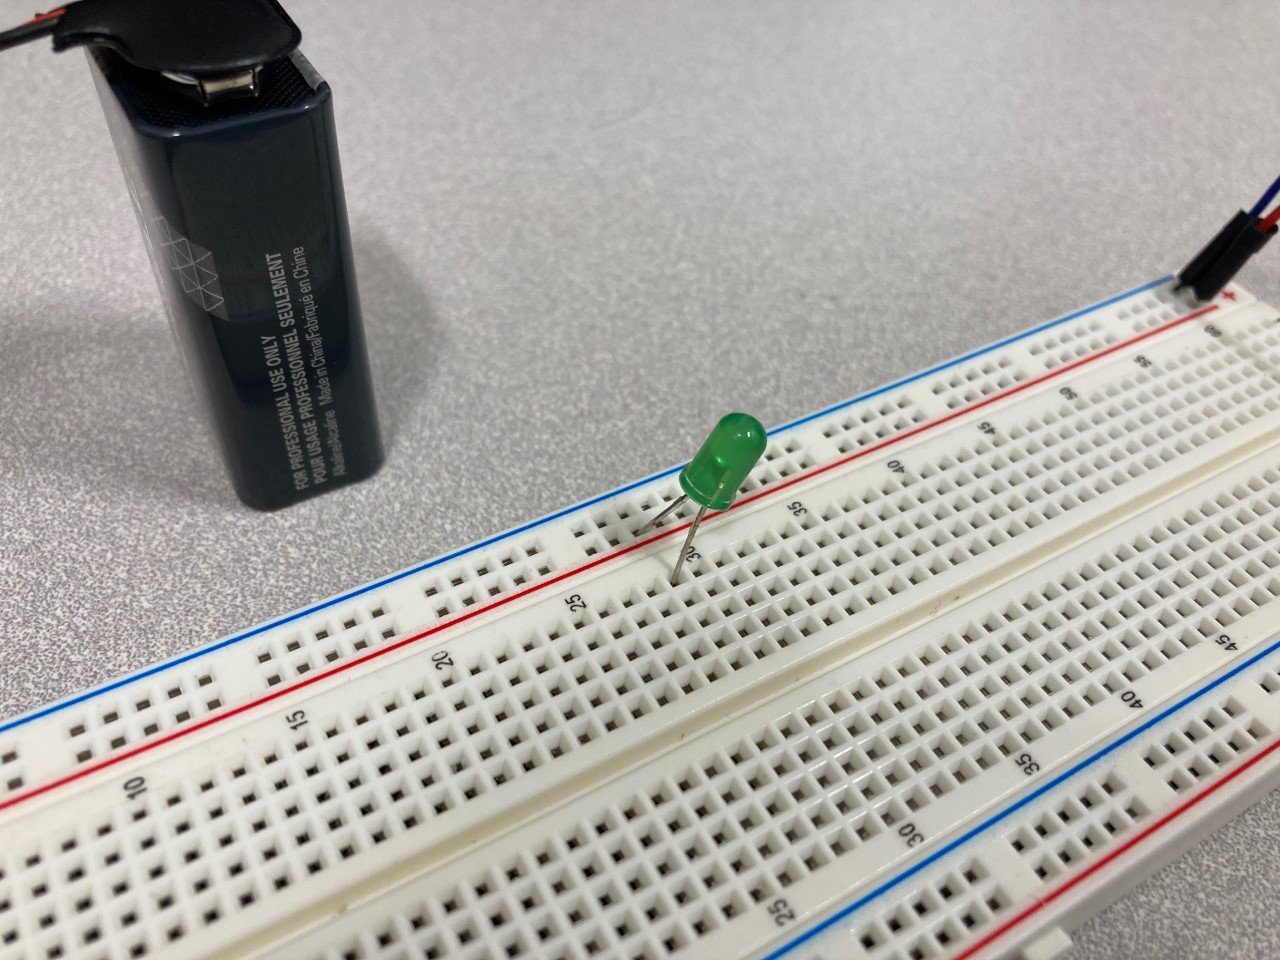
\includegraphics[width=0.8\textwidth]{protoboard_example_b}
\caption[Adding an LED to the prototyping board]{Adding an LED to the 
prototyping board. The long lead is placed in one of the holes connected
to power, and the other lead is connected to a center strip.}
\label{fig:protoboard_example_b}
\end{figure}

At this point, our LED has not lit, because it needs to form a complete circuit,
which we could do by connecting a wire from the unconnected lead to ground
(one of the blue rows). We don't want to do this, though, as the full nine
volts from the battery is probably too much for our LED. So we're going to put
a resistor in first. I'll use a 330 Ohm resistor for this exercise. I connect
one of the resistor leads into the same five hole group that the LED is 
connected to, and the other lead into a hole from a different group (putting
both leads into holes from the same group would be like connecting the two
ends of the resistor together, effectively removing it from the circuit). These
connections can be seen in Figure \ref{fig:protoboard_example_c}.
\begin{figure}[hbp!]
\centering
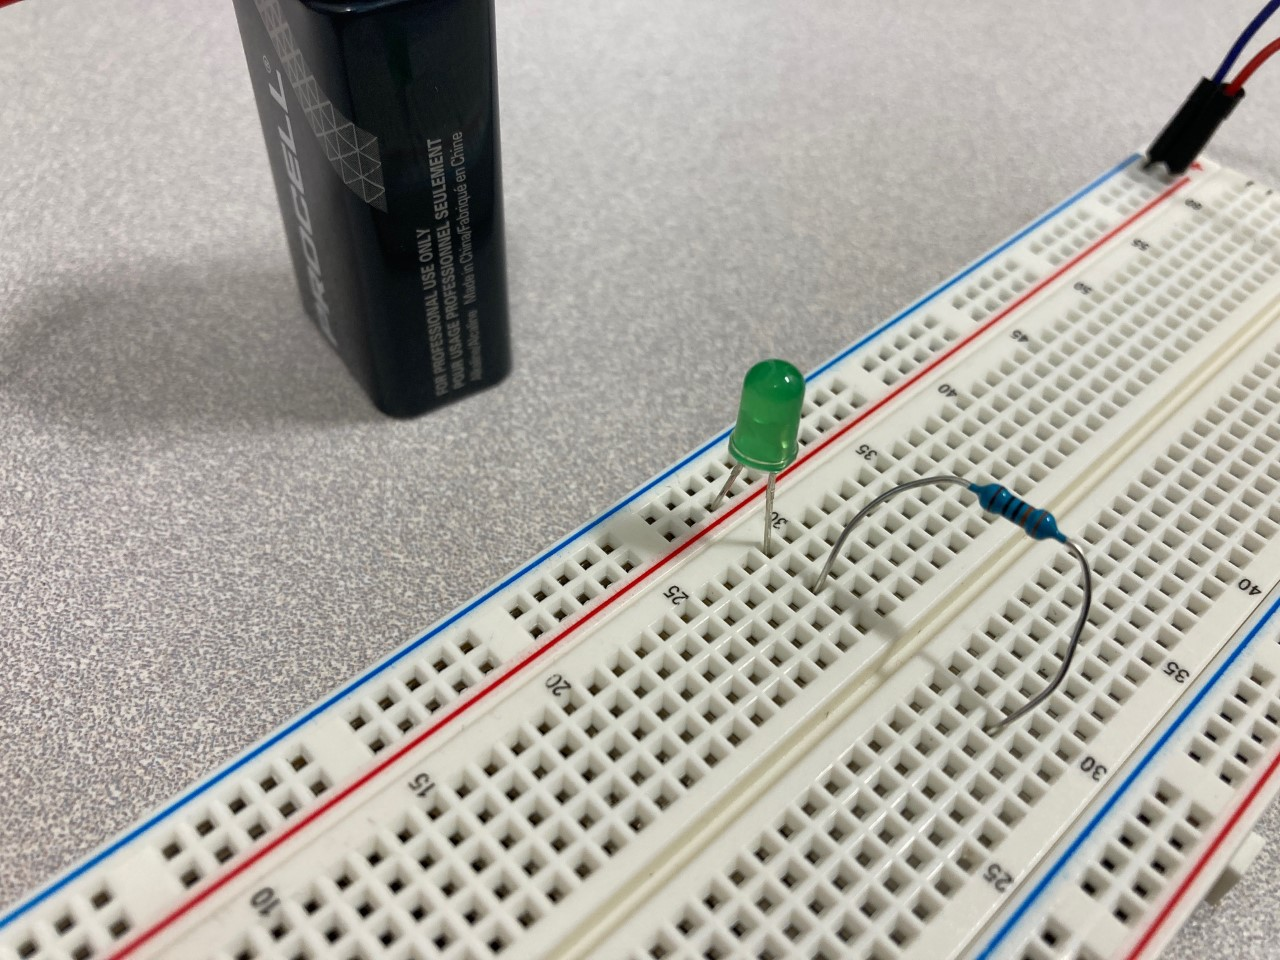
\includegraphics[width=0.8\textwidth]{protoboard_example_c}
\caption[Adding a resistor to the prototyping board]{Adding a resistor to the
prototyping board. One lead is placed in one of the holes in the same group
as the LED lead, and the other lead is connected to a different group.}
\label{fig:protoboard_example_c}
\end{figure}

Our LED is still not lit. We will now complete the circuit by adding a ground
connection. I could have done this by putting the second lead of the resistor
into one of the ground holes, but I'll instead use a wire to finish the
connection. The LED is now lit (Figure \ref{fig:protoboard_example_d})!
\begin{figure}[hbp!]
\centering
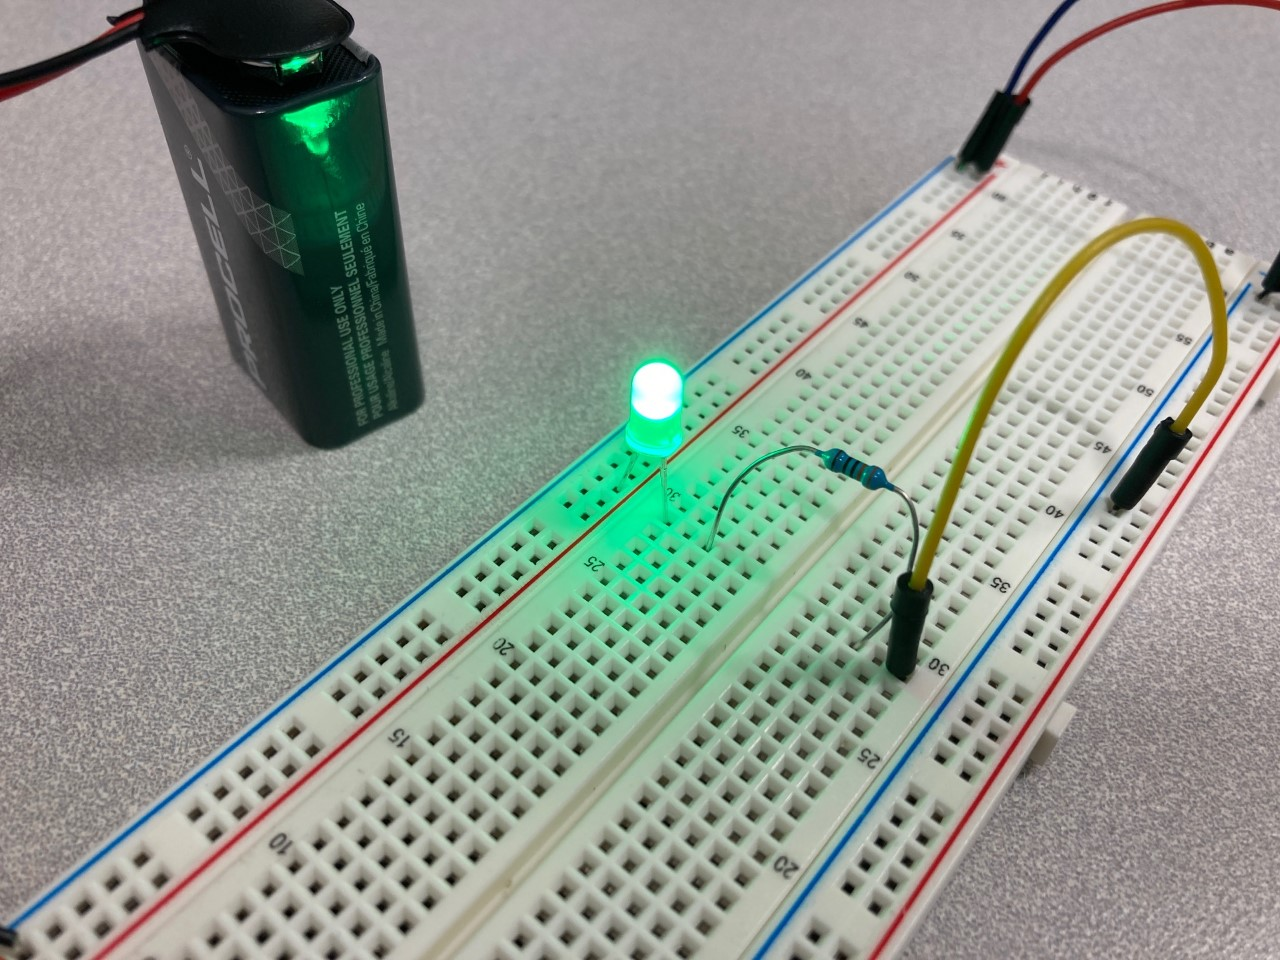
\includegraphics[width=0.8\textwidth]{protoboard_example_d}
\caption[Completing the simple LED circuit]{Completing the simple LED circuit.
One end of the yellow wire is connected to the same group as the end of the
resistor, and the other end of the wire is connected to the ground (blue)
row. Having completed the circuit, the LED is lit.}
\label{fig:protoboard_example_d}
\end{figure}

\activity{
With the exception of the 9 V battery, build the circuit from this example
on a prototyping board.
}

This concludes our example for using a prototyping board to construct a circuit.
Before this lab concludes, we are going to use our Arduino as the power source
for this circuit, and also have a little fun using the Arduino to control the
behavior of the LED. Before we do that, though, we need to talk about soldering.

\subsection{Durable circuits: soldering}

If you followed the last example carefully, you may have 
noted a few things:
\begin{itemize}
\item Using the prototyping board makes this circuit a lot larger than it 
needs to be.
\item We made electrical connections by easily sliding a lead or wire into a
hole. The wire or lead can just as easily be removed from the hole.
\item The entire thing looks like it will fall apart if I try to pick it up
and move it.
\end{itemize}
It is fairly apparent that prototyping boards are good for designing circuits
and building a prototype for testing (hence the name ``prototyping board'').
But if I am going to put this circuit to any sort of practical use, I need to
build it in a more permanent fashion. The way we do this is by electrically
``gluing'' the connections together with solder.

Solder consists of a ductile metal alloy (usually tin, silver, and/or lead) 
mixed with a small amount of material called flux. Solder has a relatively low
melting point, and is also electrically conductive. By melting a little bit of
solder between the wires or leads we want to connect, and then letting the 
solder reset, we can make a mechanically strong connection.

In order to make a mechanically strong and electrically sound connection, 
soldering must be done correctly. The process begins by making sure you have
the right equipment and that it has been properly prepared. Figure
\ref{fig:soldering_equipment} shows the elements of a good soldering station, 
including (from left to right)
\begin{itemize}
\item A soldering iron. This provides the heat to melt the solder.
\item Solder. In this case, it is provided on a spool.
\item Flux paste. Flux is what helps solder flow. Sometimes solder doesn't
have enough flux, and having a little extra paste handy can make a huge 
difference.
\item Tip cleaner. The tip of a soldering iron, after a little use, will start
get gummed up with oxides. When this happens, it doesn't conduct heat very well.
Frequent tip cleaning makes your life a lot easier!
\item Helping hands. This device includes a few clamps that can hold your work
in place, and usually also includes a magnifying glass to help you see what
you are doing. This piece of equipment is critical! Normally, when soldering a
circuit, you need to hold the circuit, the element you are soldering to it, 
the soldering iron, and the solder all at the same time. Unless you have four
hands, you'll need one of these devices!
\item Wire wick. Sometimes you make mistakes while soldering. Wire wick, when 
heated, will sop up solder so you can remove it from your work.
\end{itemize}
\begin{figure}[hbp!]
\centering
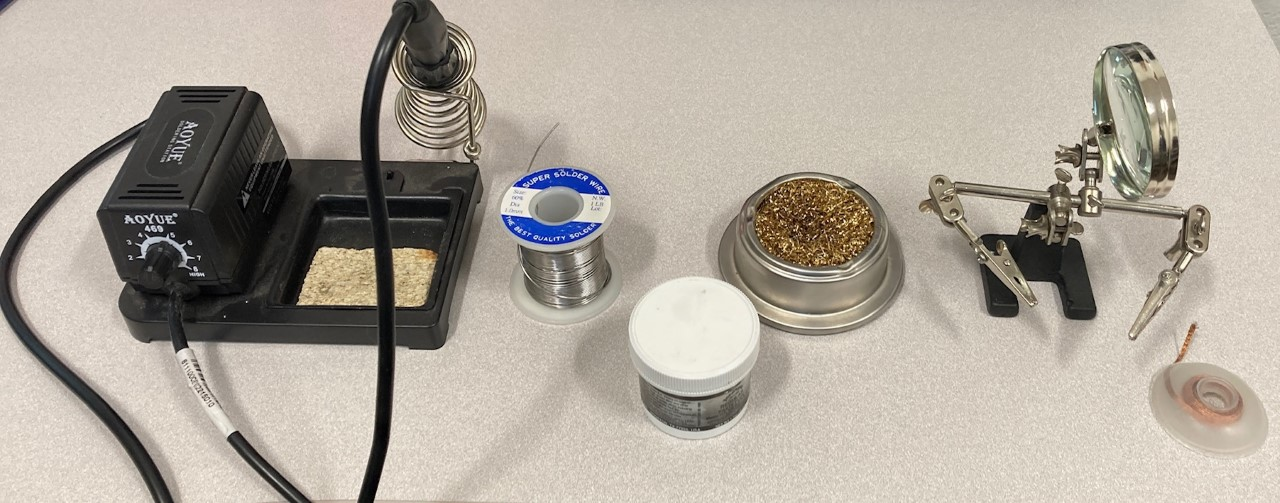
\includegraphics[width=0.8\textwidth]{soldering_equipment}
\caption[Soldering equipment]{Soldering equipment. Included here are
a soldering iron, solder, flux paste, a tip cleaner, a set of ``helping
hands'', and wire wick. See the text for a more full description of these
items.}
\label{fig:soldering_equipment}
\end{figure}

In addition to this equipment, it's also convenient to have a surface to 
solder our components on, rather than trying to solder them together directly.
A common surface is pictured in Figure \ref{fig:perfboard}, and is called a
perfboard. It's basically just a fiberglass board with a bunch of holes
(perforations) drilled in it, and the holes are lined with some sort of 
conductive material.
\begin{figure}[hbp!]
\centering
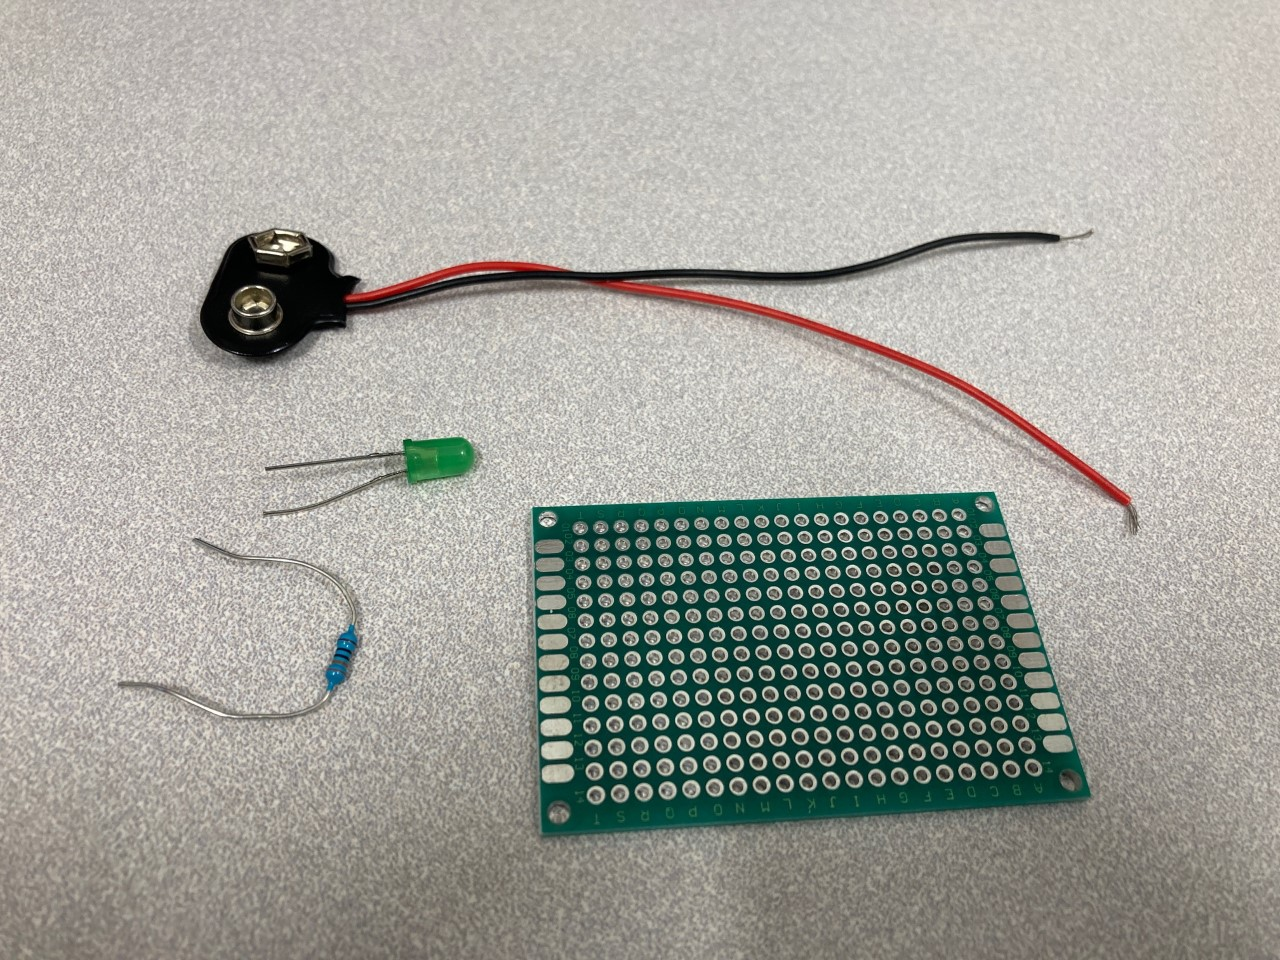
\includegraphics[width=0.8\textwidth]{perfboard}
\caption[A perfboard]{A perfboard, along with some items we will solder
together on it.}
\label{fig:perfboard}
\end{figure}

Now, let's get started. First we'll plug the soldering iron in and give it a 
few minutes to heat up. Once heated, we then want to clean and prepare the tip.
This is done by plunging the tip of the soldering iron in and out of the tip 
cleaner several times. At this point, we'll also dip the tip very briefly 
into the flux paste, and then clean the tip again. Finally, we'll melt a small 
amount of solder onto the tip, and then clean it a third time. At this point,
the tip should be clean and shining with solder, similar to Figure
\ref{fig:solder_ready}.
\begin{figure}[hbp!]
\centering
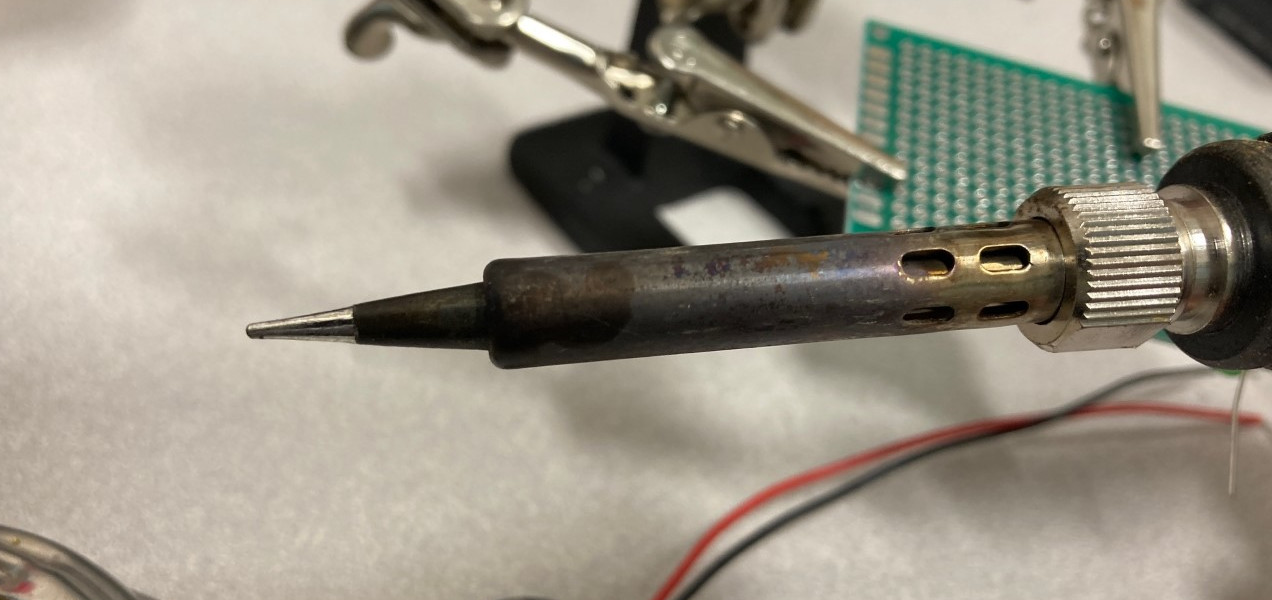
\includegraphics[width=0.8\textwidth]{solder_ready}
\caption[A clean soldering iron tip]{A clean soldering iron tip, ready for
use.}
\label{fig:solder_ready}
\end{figure}

The next step is to start putting elements on the perfboard. Components with
leads can usually be held in place prior to soldering by bending the leads on
the backside of the board. These bent leads can also conveniently be used as
wires between components as well. In Figure \ref{fig:component_preparation},
all of the components for the circuit have been placed on the boards, and 
the leads bent to make electrical connections. Normally you would only add a 
few components at a time, solder those into place, then add more.
\begin{figure}[hbp!]
\centering
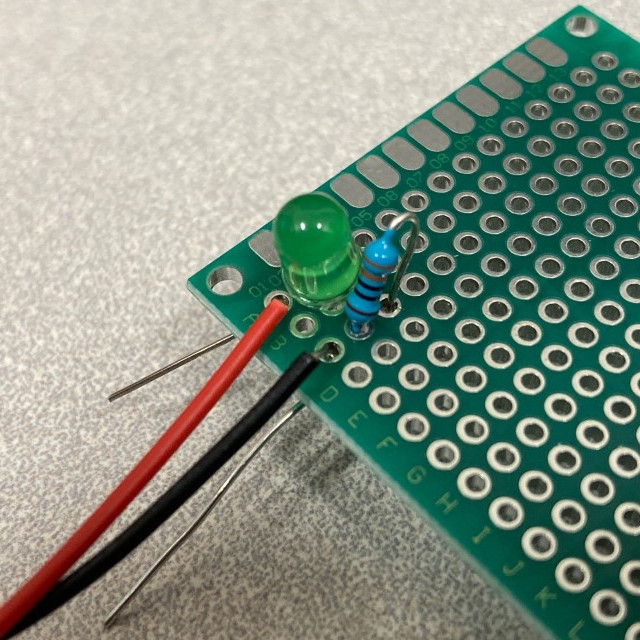
\includegraphics[width=0.4\textwidth]{component_preparation_a}
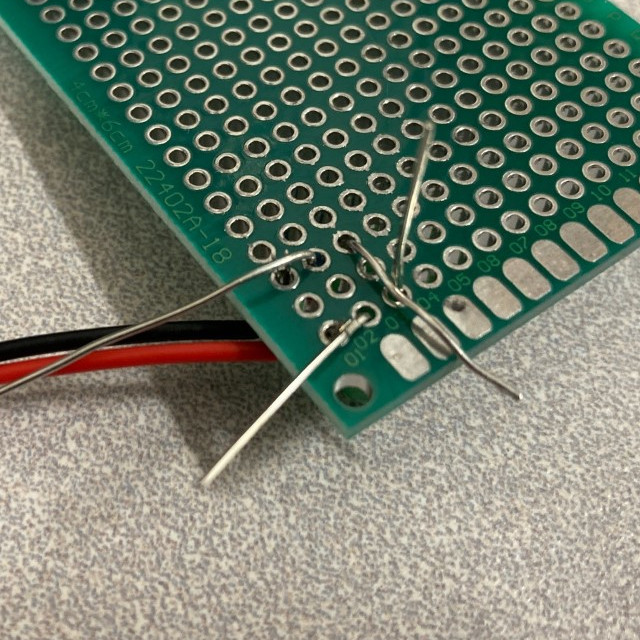
\includegraphics[width=0.4\textwidth]{component_preparation_b}
\caption[Components added to a perfboard, ready for soldering]{Components added
to a perfboard, ready for soldering. Note how, on the back side of the 
perfboard, the leads have been bent to hold the components in place as well as
act as wires.}
\label{fig:component_preparation}
\end{figure}

Now to apply the solder. Rather than trying to hold the entire spool of 
solder, it's easiest to use the soldering iron to burn off a three or so inch
segment instead. A key thing to remember is that you should
\textit{\textbf{heat the work, not the solder}}. If you just touch the solder
with the soldering iron, it will melt, and it might even transfer onto the
parts you are trying to solder. However, the flux tends to move to the 
surface of hot metal, and you'll basically end up with a ball of solder that
is insulated from the work by a thin layer of flux. This is referred to as a
\textit{cold solder} joint, and will likely not provide a lasting electrical
connection. By heating the work and then melting the solder onto the work,
you'll end up with good connections. 
\begin{figure}[hbp!]
\centering
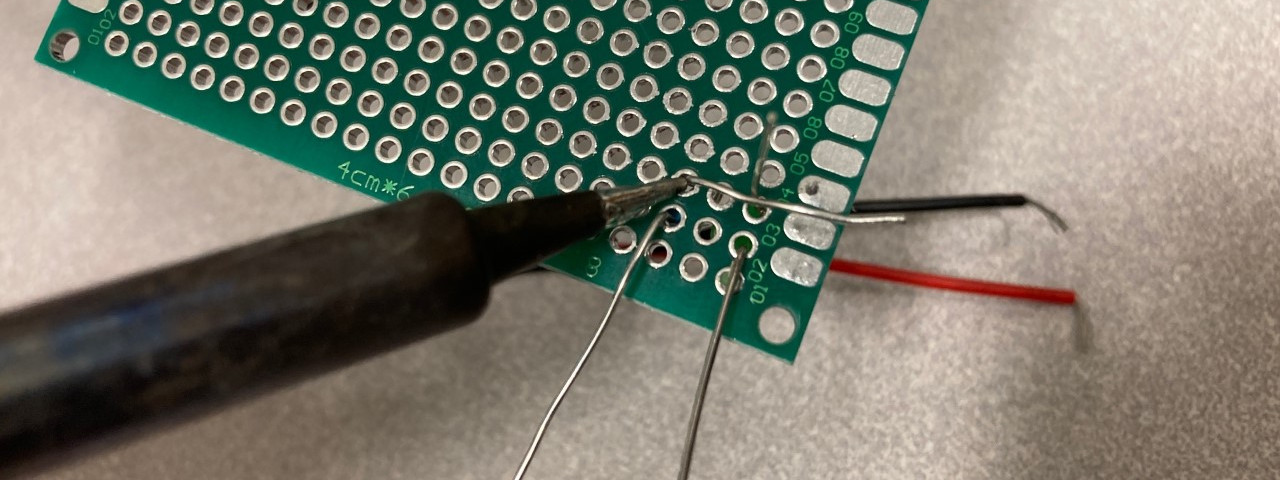
\includegraphics[width=0.8\textwidth]{heat_the_work}
\caption[Heat the work, not the solder!]{Heat the work, not the solder!}
\label{fig:heat_the_work}
\end{figure}

Once the iron is removed from the working area, the solder will cool and set
very quickly.
This process is repeated for each of the
connections. Figure \ref{fig:soldering_almost_done} shows the results with just
a few connections left to solder. In this figure, you'll note that one of the
clamps on the helping hands is holding the wire in place.
\begin{figure}[hbp!]
\centering
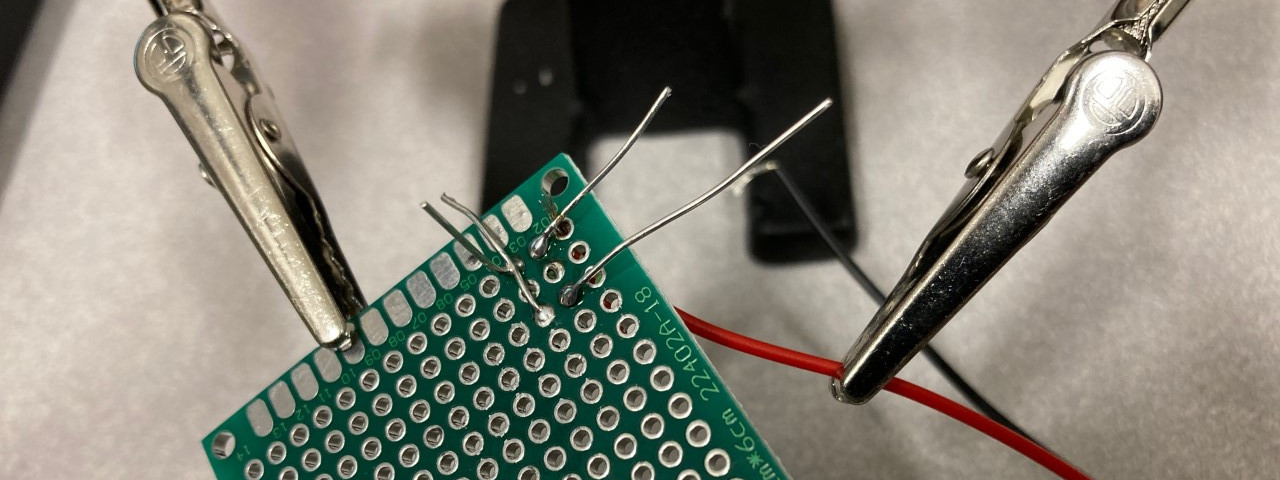
\includegraphics[width=0.8\textwidth]{soldering_almost_done}
\caption[Soldering project near completion]{The soldering project near 
completion. The connections to the 9 V battery connector still need to be
soldered. Note that one of the clamps of the helping hands is holding the red
wire in place.}
\label{fig:soldering_almost_done}
\end{figure}

Once all of the soldering is complete, you'll have some tails of wire and
component lead sticking out. Use a set of close clipping wire cutters to remove
these extra and unnecessary pieces of metal. Now our project is complete
(see Figure \ref{fig:soldering_complete}. Note that the finished product is
significantly more durable than what we had on the prototyping board, and also
significantly smaller. (The perfboard used here is 4 cm by 6 cm, and clearly a much smaller board could have been used.
\begin{figure}[hbp!]
\centering
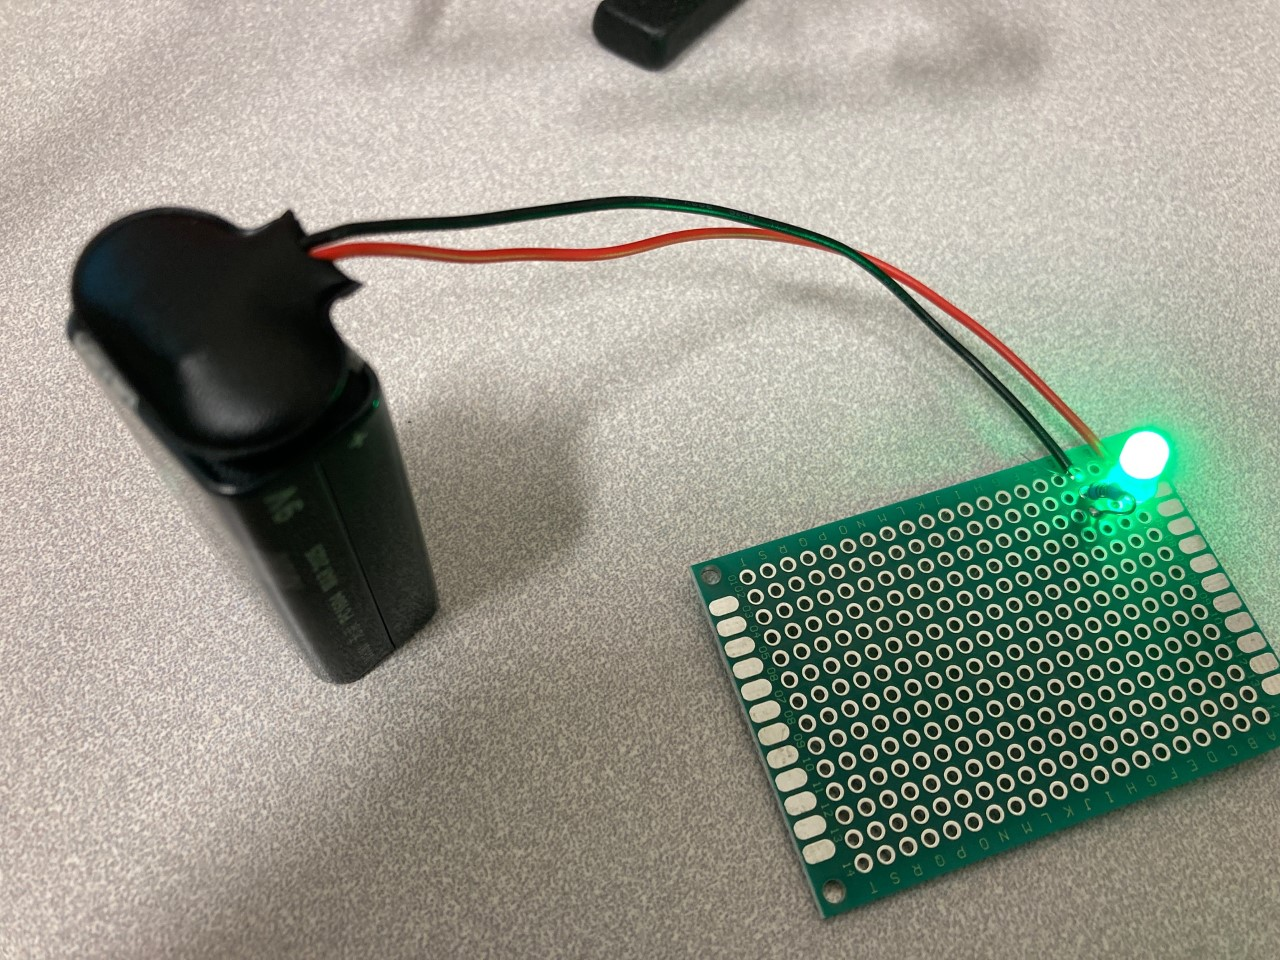
\includegraphics[width=0.8\textwidth]{soldering_complete}
\caption[The completed soldering project]{The completed soldering project.}
\label{fig:soldering_complete}
\end{figure}

When a particular circuit needs to be produced in large amounts, someone will
usually design and produce a printed circuit board, or PCB. A PCB consists of 
several layers of conductors, insulating substrates, and inks. The conducting
layers make the connections between circuit elements, so one only needs to
solder the circuit elements in place, and not worry about wiring the 
connections between them. An example of a PCB can be seen in Figure
\ref{fig:pcb}. The conducting layers are most obviously visible in the
lower left portion of the PCB.
\begin{figure}[hbp!]
\centering
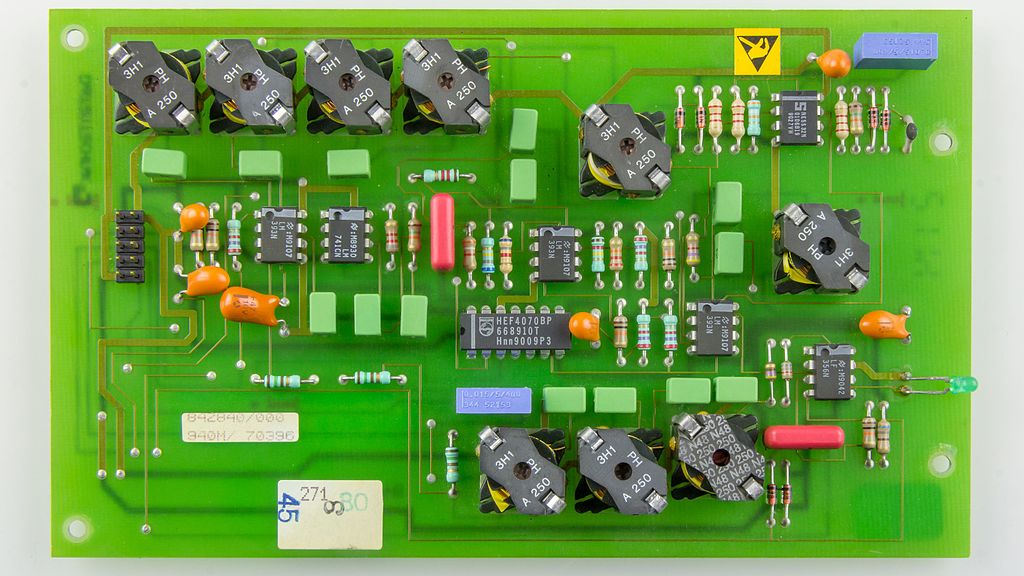
\includegraphics[width=0.8\textwidth]{pcb}
\caption[A printed circuit board]{An example of a printed circuit board,
populated with components. The conducting layers are highly visible in the 
lower left portion of the board.}
\label{fig:pcb}
\end{figure}

The type of soldering presented here is called ``through hole'' soldering, so 
named because leads from the components are placed through holes and then
soldered into place. Smaller circuit elements are often soldered directly to
pads on the surface of a PCB. This type of soldering is called ``surface
mount'', and is somewhat more difficult to perform. We will not be doing any
surface mount soldering in this lab. Both through hole and surface mount
connections can be seen in Figure \ref{fig:pcb}. The diodes, resistors, and
inductors (all cylindrically shaped components with one or more bands around 
their circumferences) have been connected with through hole soldering. The
ICs (the black boxes) are connected via surface mount.

\activity{
Successfully complete three or more soldering connections.
}

Now that we've seen how to design, build, and solder circuits, let's look at
controlling our circuit using an Arduino.

%%%%%%%%%%%%%%%%%%%%%%%%%%%%%%%%%%%%%%%%%%%%%%%%%%%%%%%%%%%%%%%%%%%%%%%%%%%%%%%%

\section{Arduino Circuit Control}

Let's start our study of computer control by controlling something simple
with an Arduino DAQ: the LED circuit that we constructed earlier on the
prototyping board. Our objective is to use the Arduino to turn the LED on and 
off. 

\subsection{Attaching the Arduino to the circuit}

Connecting the Arduino to our LED circuit built earlier is quite simple. We 
will be using the digital I/O ports found on one side of the Arduino, as 
seen in Figure \ref{fig:arduino_left}. In this figure, you will see that 
these ports are numbered, starting from the left, 1-13, GND, AREF, SDA, and
SCL. Of those ports, the ones of greatest interest to us today are the numbered
ports and the GND port (GND stands for ``ground''). The numbered ports will be
our voltage source, and the GND port will be our ground connection (akin to the
negative terminal of a battery).
\footnote{You will note that the
Arduino is assembled on a printed circuit board. Can you identify which 
components were attached by through hole v. surface mount soldering?}
\begin{figure}[hbp!]
\centering
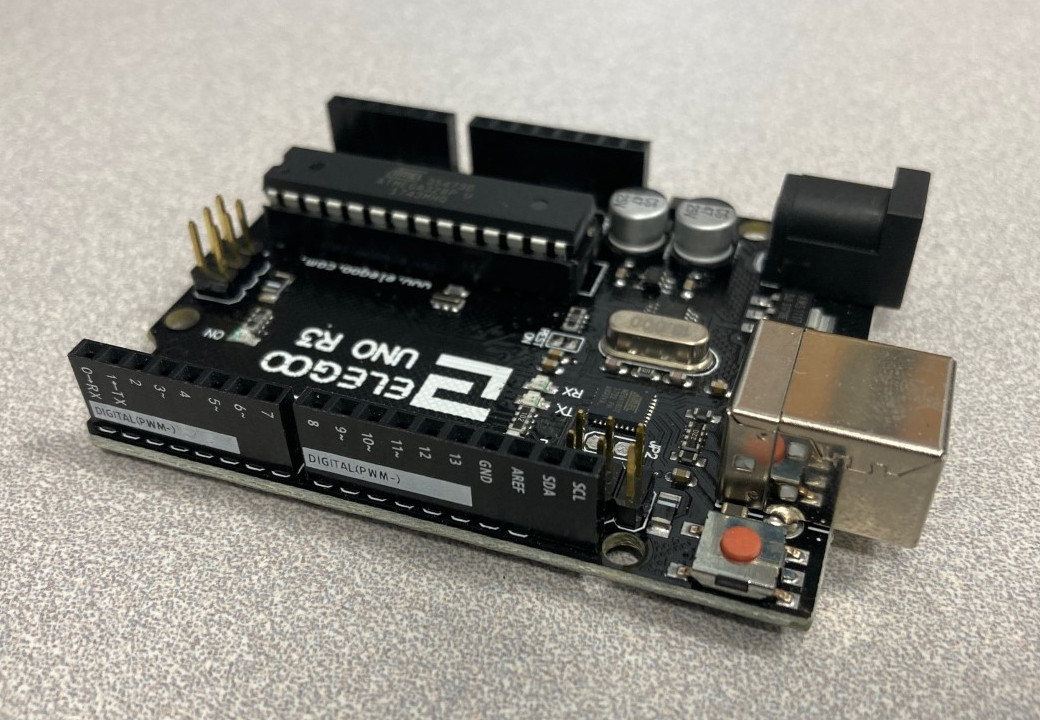
\includegraphics[width=0.8\textwidth]{arduino_left}
\caption[The digital ports on an Arduino]{The digital ports on an Arduino.}
\label{fig:arduino_left}
\end{figure}

To connect the Arduino to our circuit, we place a wire into port 13 (or any
of the other numbered ports, but for the example here we're going to use port
13), and the other end of the wire into the red row of our prototyping board.
This is the same way we connected the positive terminal of the battery earlier.
A second wire connects the GND port of the Arduino to the blue row, where we
had previously connected the negative terminal of the battery. These 
connections can be seen in Figure \ref{fig:arduino_connected}.
\begin{figure}[hbp!]
\centering
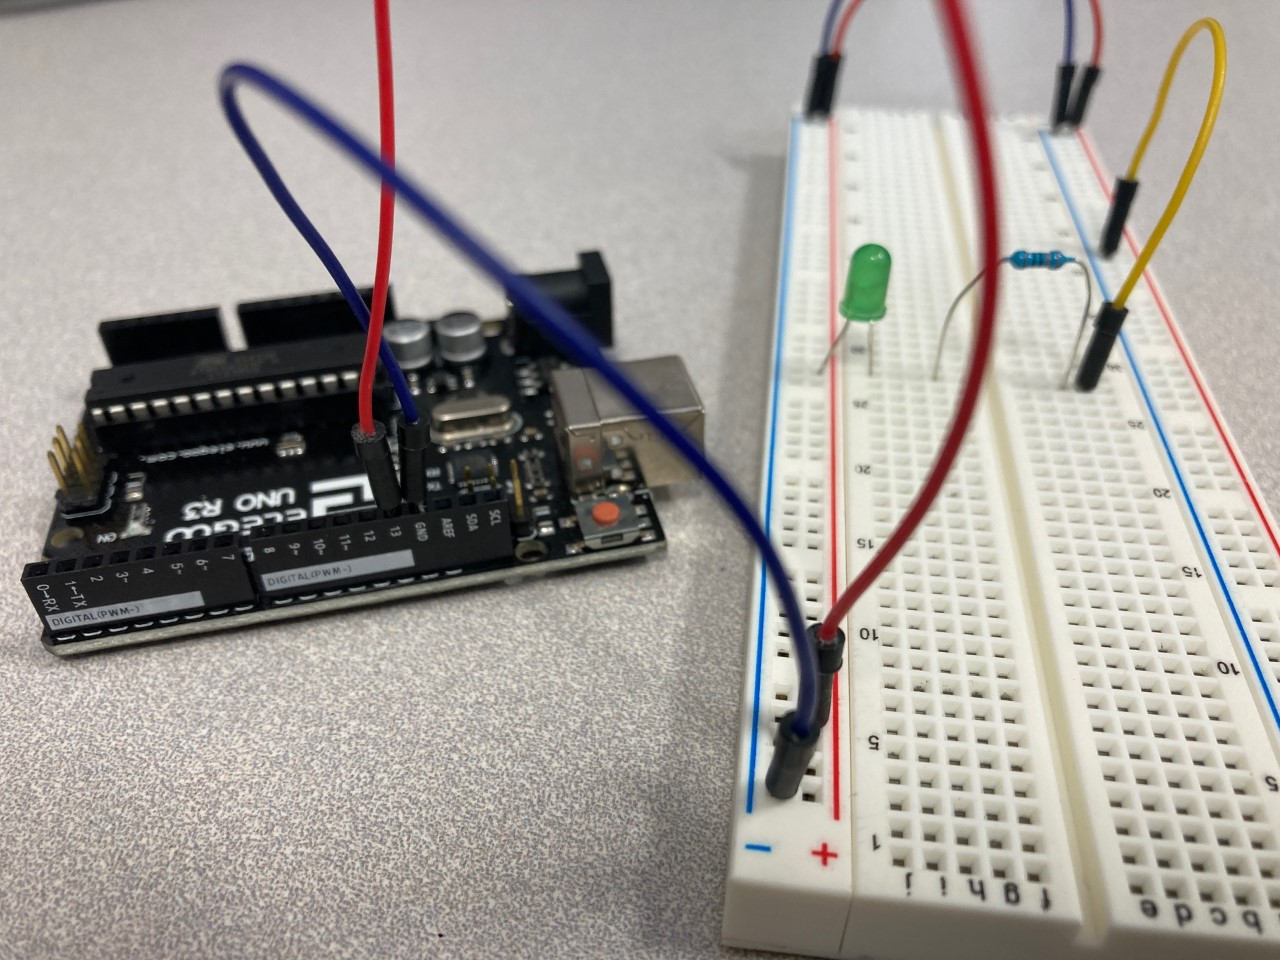
\includegraphics[width=0.8\textwidth]{arduino_connected}
\caption[The Arduino connected to the LED circuit]{The Arduino connected to
the LED circuit. The connections are described in the text.}
\label{fig:arduino_connected}
\end{figure}

A discussion about ``ground'' is warranted here. The name ``ground'' is quite
literal, in a way. The Earth is big, and can act as a giant sink for electric
potential. More importantly for us, the ground provides a reference that we
can measure electric potentials with respect to. The numbered ports on the
Arduino are going to provide five Volts of potential relative to ground. How 
does the Arduino know what the ``ground'' is? Because it will also be connected
to our computer. The plug on our computer has a ``ground'' prong (the round
prong), which (if the building you are in is wired to applicable codes) is 
electrically connected to a copper rod that has been pounded down into the
ground.

From this point on, we will no longer provide pictures of the circuits that
we build (usually). Circuits are typically represented using schematic diagrams
instead of pictures. A schematic diagram is a simplified representation of
a circuit. Each type of component has a symbol associated with it. Connections
between components are represented with lines. Connections to things outside
of the circuit are represented by pins. As an example, the circuit we have
just built is represented in Figure \ref{fig:blink_circuit}. The rectangle 
labeled with ``R1'' is our resistor, and you can see the resistance value
next to the label. The arrowhead terminating on a line, labeled ``D1'', 
represents a diode. The smaller arrows leaving the diode indicate that this 
is a light emitting diode, or LED (also indicated by the label). The pinouts to 
the Arduino are labeled ``J1'' and ``J2'', and their intended connections are
also included on their labels. Part of the fun of building electric circuits is 
constructing a physical circuit 
from the information given in the schematic!
\begin{figure}[hbp!]
\centering
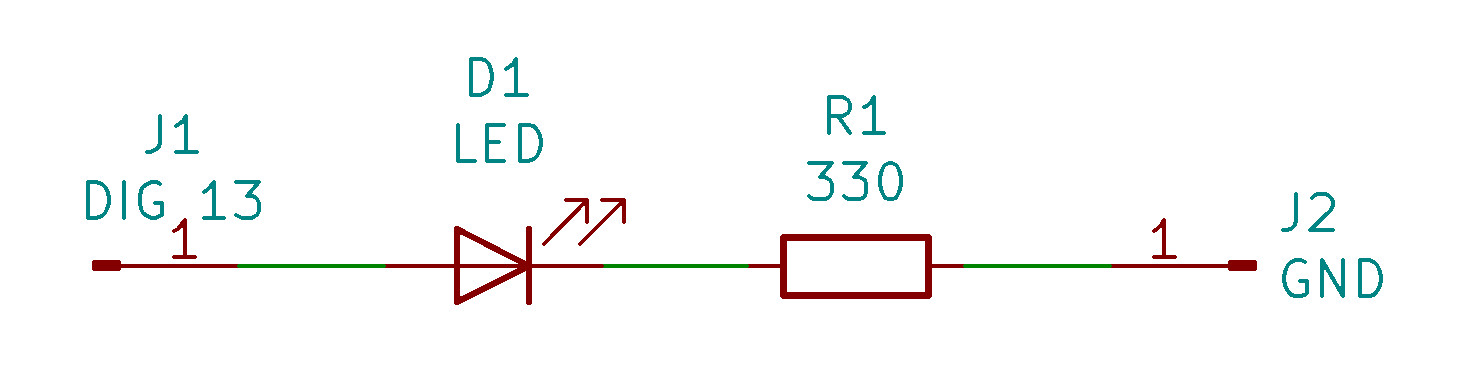
\includegraphics[width=0.8\textwidth]{blink_circuit}
\caption[Schematic diagram for the blink circuit]{Schematic diagram for the
blink circuit. The rectangle symbol represents the resistor, and the other
symbol represents the LED. The pinouts to the Arduino are labeled at the ends.
See the text for a more full description.}
\label{fig:blink_circuit}
\end{figure}

At this point, the LED is still out. There are two reasons for this. First, we
have not yet provided power to the Arduino. Second, we have not yet told the 
Arduino to turn on the LED. Providing power to the Arduino can be done in
several ways. For today, we will simply connect the Arduino to our computer
using a USB cable. (We need this USB connection in order to program the
Arduino, also.)

\subsection{The Arduino sketch: an introduction}

We now have our ``hardware'' built for a blinked LED. We still need to 
give instructions to our Arduino so it knows how to use pin 13 and GND to
make the LED blink. The Arduino has a small computer on board, and we need
to upload a computer program to the Arduino in order to tell it what to do.

You have likely already written programs at some point in your education. 
Common programming languages include Python, Java, and C++. Arduino programs
are similar to other programming languages\footnote{The Arduino programming
language is essentially C++ with some modification. If you are already familiar
with C or C++, Arduino programming will feel quite comfortable.}. 
They have loops and conditional statements, but additionally have special code
for controlling the Arduino.

Most Arduino codes are very short. For today's code, we just need to tell the
Arduino what to turn on and when, and when to turn it back off again.

Every Arduino program has two required parts: the \code{setup()} function and
the \code{loop()} function. When the Arduino is powered on, the \code{setup()}
function is executed once. As the name of the function implies, it is typically
used to set up variables or environments that the rest of the program will use.
Once the \code{setup()} function has been executed, the \code{loop()} function
is executed. This is where most of the action happens in the program. This 
function is repeated over and over again until the Arduino is powered down.

Let's introduce the commands we will use for this lab. Each digital output on
the Arduino has a number. The code will need to know which pin number we are
working with. There are two ways we can do this. The first is to define a 
variable of type integer (int) and set it equal to the pin number. The code to
do this would typically be written before the \code{setup()} function, and 
would look something like this:
\begin{lstlisting}[language=Arduino] 
int ledPin=13;
\end{lstlisting}
The other way we can do this is with a \code{\#define} 
statement at the beginning of the code,
before the \code{setup()} function.
A \code{\#define} statement 
simply tells the compiler (the thing that turns our human
readable code into binary code that the processor understands) to replace the
defined name with whatever follows in the definition. Such a definition would
look something like this:
\begin{lstlisting}[language=Arduino] 
#define ledPin 13
\end{lstlisting}

As stated before, most of the action of the program happens in the
\code{loop()} function. In our case, our loop function needs to turn on
the digital pin our LED is connected to, wait for a short while, turn it off
again, and then wait some more.
A digital pin on the Arduino can be set to a LOW voltage (zero Volts relative
to ground) or a HIGH voltage (+5 V relative to ground). Each digital pin that
we use also needs to be set up for output or input. This is done with a 
``pinMode'' statement. For example, to set pin 13 to output, I would use the 
following in my \code{setup()} function, recalling that we had previously
set \code{ledPin} to a value of 13:
\begin{lstlisting}[language=Arduino] 
    pinMode(ledPin,OUTPUT);
\end{lstlisting}
If I had wanted to set up the pin for input, I would simply replace the
\code{OUTPUT} with \code{INPUT}.

To set the pin to LOW or HIGH voltage, use a digitalWrite command:
\begin{lstlisting}[language=Arduino] 
    digitalWrite(ledPin,LOW);
    digitalWrite(ledPin,HIGH);
\end{lstlisting}
And, finally, to leave the light on (or off) for a while, we can use
a delay command, where the argument to the command gives the delay time in
milliseconds:
\begin{lstlisting}[language=Arduino] 
    delay(100);
\end{lstlisting}

Altogether, our Arduino code for blinking lights would read as follows:
\begin{lstlisting}[language=Arduino] 
#define ledPin 13

void setup() 
{
    pinMode(ledPin, OUTPUT);
}

void loop() 
{
    digitalWrite(ledPin,HIGH);
    delay(100);
    digitalWrite(ledPin,LOW);
    delay(100);
}
\end{lstlisting}
There are a few things to note about the syntax. First, every line of command
within the code is terminated with a semicolon. This tells the compiler that the
command is complete, and also allows us to continue a command onto a second
or third line when needed. The only exception is the \code{\#define} statement.
Second, any grouped set of command, be that in a function, a loop, or a 
conditional statement (the latter two do not appear in this code) are 
encapsulated in a set of curly braces. Once again, this tells the compiler 
where the set of commands begins and ends.

The code above, while it will make the Arduino behave the way we want, is not
ideal. It is missing a \textit{\textbf{very critical}} part: comments. You 
should always include abundant comments in your code, including a comment 
block at the top describing what the code does overall, comments describing
each variable you declare or define, and comments that describe each part of
the algorithm in the code. Why do you want so many comments? Some people would
say that you include comments to help other people understand what your code
is doing. The reality is, though, that you put the comments in your code so 
that \textit{\textbf{you}} can remember what your code is doing when you 
come back to it weeks or months later. For this lab course, comments are 
required in all of your code.

In the Arduino language, single line comments can be started with a double
forward slash ``//''. Block comments can also be started with a ``/*'' and 
ended with a ``*/''.
Once I've included adequate comments, my code will look something like this
\begin{lstlisting}[language=Arduino] 
/////////////////////////////////////////////////////////
// Arduino sketch to blink one LED
//   Written by (your name would go here)
//   Feb. 6, 2017 
/////////////////////////////////////////////////////////

// Define the pin we are using for output

#define ledPin 13

/////////////////////////////////////////////////////////
// The arduino setup function comes next. We need to set
// up pin 13 for output. 
/////////////////////////////////////////////////////////

void setup() 
{
    pinMode(ledPin, OUTPUT);
}

/////////////////////////////////////////////////////////
// Now comes the loop function. We simply turn on the 
// LED, wait for a while, turn off the LED, and wait 
// some more.
/////////////////////////////////////////////////////////

void loop() 
{
    digitalWrite(ledPin,HIGH);  // Turn on the LED
    delay(100);                 // Wait 100 ms
    digitalWrite(ledPin,LOW);   // Turn off the LED
    delay(100);                 // Wait 100 ms
}
\end{lstlisting}

\subsection{Compiling and uploading the sketch}

So that's how you write Arduino code. How do you get it to your Arduino? 
There is a special integrated development environment (IDE) for 
programming our Arduino. The IDE can be seen in Figure \ref{fig:ide}.

We will need to install this IDE before we can communicate with our 
Arduino. To do so we use a web browser to go to\\

\href{https://www.arduino.cc/en/Guide/HomePage}{https://www.arduino.cc/en/Guide/HomePage}\\

\noindent and choose to install the Arduino IDE for your computer. 
In the figure, you will see two important buttons on the left side of the 
toolbar. One is the ``compile'' button. The Arduino cannot interpret the 
human readable code that we write in the IDE. It needs to have the code 
translated into binary (ones and zeroes) that digital logic circuits understand.
This translation process is called ``comiling''. As the code is compiled, the
Arduino software looks for errors in the code. If there are errors, it will
tell you at this point. This way we can correct the errors before we send 
the compiled instructions to the Arduino.
\begin{figure}[hbp!]
\centering
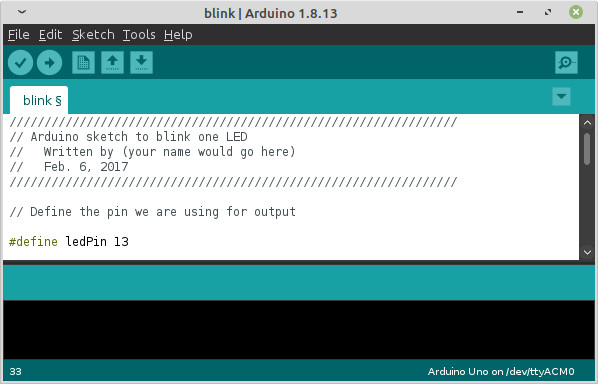
\includegraphics[width=0.8\textwidth]{ide}
\caption[The Arduino IDE]{The Arduino IDE. The compile and upload buttons are
found at the left side of the tool bar.}
\label{fig:ide}
\end{figure}

We also need a way to send our code to our Arduino and that is what the
upload to Arduino button does. Once the code is compiled without errors,
connect the USB\ cable to the Arduino and push the upload button. Once the 
code is uploaded to the Arduino, we should see some blinking lights!

One last thing to note: Arduino programs are called ``sketches''. As you 
keep your lab notebook, you should always include a copy of your sketch, along
with notes on how you got it to work. It's also a good idea to include 
pictures and schematics of any circuits you have constructed.

\activity{
Build your own clone of the blinking light circuit described in this section
by doing each of the following:
\begin{itemize}
\item Construct the LED circuit on a prototyping board.
\item Connect the Arduino to the LED circuit and to your computer.
\item Write, compile, and upload the ``blink'' sketch to the Arduino.
\item Verify that the circuit is working correctly.
\end{itemize}
}

%%%%%%%%%%%%%%%%%%%%%%%%%%%%%%%%%%%%%%%%%%%%%%%%%%%%%%%%%%%%%%%%%%%%%%%%%%%%%%%%

\section{Adding More Complexity}

Now it's your turn to practice these skills by designing a building a new
circuit. Our objective is to build an Arduino
controlled circuit that does the following:
\begin{itemize}
\item Increments a counter every half second.
\item Turns on a red LED only when the counter is an even number.
\item Turns on a yellow LED only when the counter is a multiple of three.
\item Turns on a green LED only when the counter is a multiple of five.
\item Turns on a blue LED only when the counter is a multiple of seven.
\end{itemize}
Most of hardware setup will be the same, but we will be using multiple
digital pins on the Arduino (one for each LED). We will have to abandon our 
nice $+5\unit{V}$ top row on our prototyping board as our connection to
pin 13, because we need multiple pins and we need them to operate independently.
Instead, we can wire pin 13 of our Arduino directly to the top lead of one LED, 
wire pin 12 to the top lead of another LED, and so on. It's OK for each branch
of this circuit to share the same ground connection.

To do this, we will need a counter variable. The variable \code{i} is a common
choice. You'll want to declare this variable as an integer at the beginning of
your sketch, and set its value equal to zero. At the end of the loop statement,
you can increment the counter using 
\begin{lstlisting}[language=Arduino]
    i=i+1;
\end{lstlisting}
or
\begin{lstlisting}[language=Arduino]
    i++;
\end{lstlisting}

You will also need to make the Arduino to some math. Specifically, you'll need
to test whether the counter is currently a multiple of the desired number.
This can be done using a conditional statement. In the Arduino language, 
conditional statements will take on the following form:
\begin{lstlisting}[language=Arduino] 
    if(a<b)
    {
        firstFunction();
	delay(100);
	secondFunction();
    }
    else if(a<c)
    {
        anotherFirstFunction();
	delay(200);
    }
    else
    {
        finalFunction();
    }
\end{lstlisting}
Each part of the condition includes a test statement found in the parentheses.
If the statement is true, the code included in the curly braces that follow
will be executed. In this example, if \code{a>b} evaluates true, then the
\code{firstFunction}, \code{delay}, and \code{secondFunction} will be 
executed in order. It will then skip over the rest of the code in the example.
If \code{a>b} evaluates false, the code will procede to the \code{else if}
portion of the conditional, executing the \code{anotherFirstFunction} and 
\code{delay} functions provided that \code{a<c} evaluates true. If neither
of those test statements evaluate true, then the \code{finalFunction} function
will be evaluated. You will need to use conditional statements in this exercise.

You will also want to use a mathematical operator called the modulus,
represented by a ``\code{\%}'' symbol. The operator divides the first operand
by the second and returns the remainder. For example, \code{23\%5} would 
return \code{3}. This operator can be used in a conditional statement to see
if one number is a multiple of another as in
\begin{lstlisting}[language=Arduino] 
    if(i%3==0)
    {
        // The variable i is a multiple of 3.
    }
    else
    {
        // The variable i is not a multiple of 3.
    }
\end{lstlisting}

Again, save your sketch and take a photo of 
your hardware. Place a copy of 
both in your lab notebook along with notes on how you got it to work. Make
sure others at your table are able to get their circuit to work also.

\activity{
Using the Arduino and prototyping board, construct a circuit with all of the 
following characteristics:
\begin{itemize}
\item Increments a counter every half second.
\item Turns on a red LED only when the counter is an even number.
\item Turns on a yellow LED only when the counter is a multiple of three.
\item Turns on a green LED only when the counter is a multiple of five.
\item Turns on a blue LED only when the counter is a multiple of seven.
\end{itemize}
}

% NOTE: In previous versions of the textbook, two additional activities were 
% included in which the students would make the light blink in a Fibonacci 
% sequence. One author (Kevin) noted that, since the students were just
% copy/pasting the code, they weren't getting a whole lot from this, other
% than noting that the Arduino can do math. I've included some additional
% processing in the previous activity. Additionally, because I've now included
% the section and activity on soldering, they may not have sufficient time to
% do these last activities. Hence, I have excluded them from this version.
% However, the original code is included below.

% \section{Third Computer Control: Two LED blink using math}

% Let's leave our hardware alone in the two LED setup from the last section.
% And let's make the LED's blink the same way. But this time, let's calculate
% when they should be on or off. Why would we do this? Because sometimes in
% computer control of experiments we need to turn something on or off based on
% a calculation. You may have your computer watching to make sure the
% experiment doesn't get too hot or cold. The Arduino can bring in temperature
% information, but you would have to write the code to tell it to turn off the
% heater when your experiments gets to hot and to turn it on when it gets too
% cold. This could be done with a mathematical comparison. We will use such a
% comparison in the next sketch.

% Suppose we want to know if a number is even or odd. Even numbers are evenly
% divisible by $2.$ We could divide a number by $2$ and see if the remainder
% is zero. Our Arduino language has a good set of mathematical functions. The
% remainder function is a \textquotedblleft \%\textquotedblright\ sign. For
% example 
% \begin{eqnarray*}
% 3\%2 &=&1 \\
% 6\%2 &=&0
% \end{eqnarray*}%
% Let's have one light turn on if a number is even, then switch to the other
% light if the number is odd.

% In our code we will introduce a variable, $i,$ that we will increment (add
% one to) every time the loop runs. So the first time the Arduino loop runs it
% will be zero (even) and the next time 1 (odd) and the next time 2 (even) and
% the next time 3 (odd) and so on. If you studied Python you would call such a
% variable an \textquotedblleft integer\textquotedblright\ and might even know
% to call it a \textquotedblleft loop counter.\textquotedblright

% In our Arduino sketch we will test to see if $i$ is even in an if-statement.
% If-statements go like this
%  \begin{lstlisting}[language=Arduino]
%  if (test condition ) {
%    do something;
%  }
%  else {
%    do something else;
%  }
%  \end{lstlisting}

% Notice that the parts of the if-statement need curly braces. Our condition
% to test is
%  \begin{lstlisting}[language=Arduino]
% i % 2 == 0
%  \end{lstlisting}

% Note that there are two equals signs. That makes it a test for equality
% rather than an assignment. So we will have an if-statement like this
%  \begin{lstlisting}[language=Arduino]
% if (i % 2 == 0 ) {
%  digitalWrite(ledPin1,HIGH);
%  digitalWrite(ledPin2,LOW);
%  delay(1000);
%  }
%  else {
%  digitalWrite(ledPin1,LOW);
%  digitalWrite(ledPin2,HIGH);
%  delay(1000);
%  }
%  
%  \end{lstlisting}

% One last addition, our Arduino language has a shortcut for the statement
%  \begin{lstlisting}[language=Arduino]
% i=i+1
%  \end{lstlisting}

% It is simply
%  \begin{lstlisting}[language=Arduino]
% i++
%  \end{lstlisting}

% We will use this to make $i$ increase by one each time the loop runs. The
% whole code might look like this.
% \lstinputlisting[language=Arduino]{Code/IntroBlink2LEDs_Math.ino}



% Again save your sketch. You should probably say in your lab notebook that
% you used the previous hardware setup. You might want to describe in your lab
% notebook how the mathematical algorithm works.

% \section{Fourth Computer Control: Two LED blink in the Fibonacci sequence}

% Suppose instead of LED\ lights we had large radio transmitters. And suppose
% we were part of the Search for Extra-Terrestrial Intelligence (SETI). We
% wish to send a message to any intelligent life that they would understand.
% Intelligent life probably would be able to do mathematics and would
% understand how mathematics occurs in nature. One sequence of numbers that
% occurs over and over again in nature was discovered by Fibonacci. Let's
% blink our LED\ lights (representing those powerful radio transmitters) in
% the Fibonacci sequence.

% We need to know now to calculate the Fibonacci sequence. One method is to
% know that the sequence goes like this%
% \begin{equation*}
% 0,1,1,2,3,5,8\ldots
% \end{equation*}%
% and that we can find the next number in the sequence by choosing $f_{1}=0$
% first, then $f_{2}=1$ then using the formula 
% \begin{equation*}
% f(x-1)\ +\ f(x-2)
% \end{equation*}%
% Let's see that this works. For the first of the sequence, we just write the $%
% 0.$ For the second we just write the $1.$ Then for the third 
% \begin{eqnarray*}
% f_{3} &=&f_{2}+f_{1} \\
% &=&1+0 \\
% &=&1
% \end{eqnarray*}%
% So far so good. Let's try the next in the sequence%
% \begin{eqnarray*}
% f_{4} &=&f_{3}+f_{2} \\
% &=&1+1 \\
% &=&2
% \end{eqnarray*}%
% Again it worked. For the next one%
% \begin{eqnarray*}
% f_{5} &=&f_{4}+f_{3} \\
% &=&2+1 \\
% &=&3
% \end{eqnarray*}%
% and though we won't prove it, it works for every member of the sequence. See
% if you can figure out how to write this code. An example is given below, but
% see if you can figure out what the code should be.

% This example is a much more complex version of a mathematical based computer
% control.
% \lstinputlisting[language=Arduino]{Code/IntroFibonacci.ino}
% % \begin{lstlisting}[language=Arduino]
% %/////////////////////////////////////////////////////////
% %// code to blink two LED's using a mathematical expression
% %// to determine when they should light. Note that the
% %// Arduino code is closer to C++ than python.
% %/////////////////////////////////////////////////////////
% %int ledPin1=13;
% %int ledPin2=12;
% %int i=0; //loop counter
% % 
% %/////////////////////////////////////////////////////////
% %int fib_count=0; // number of blinks based on Fibonacci
% %int i_max=10; // maximum Fibonacci number before 
% % // starting over
% % 
% %/////////////////////////////////////////////////////////
% %void setup() {
% % // put your setup code here, to run once:
% % pinMode(ledPin1, OUTPUT);
% % pinMode(ledPin2, OUTPUT);
% % } 
% % 
% %int fib(int x) {
% % // calculates the Fibonacci sequence using recursion
% % if (x==0) 
% %    return 0;
% % if (x==1)
% %   return 1;
% %   return fib(x-1) + fib(x-2);
% % } 
% % 
% %/////////////////////////////////////////////////////////
% %void loop() {
% % // put your main code here, to run repeatedly:
% % // blink the LED's with the number of blinks being 
% % // the Fibonacci sequence.
% % fib_count=fib(i);
% % if (i % 2 == 0 ) {
% %   // turn off one light
% %   digitalWrite(ledPin2,LOW);
% %   // now blink the second light fib_count times 
% %   for (int n=0; n<fib_count; n++) { 
% %      digitalWrite(ledPin1,HIGH);
% %      delay(100);
% %      digitalWrite(ledPin1,LOW);
% %      delay(100);
% %   }
% % }
% % else {
% %   // turn off the other light
% %   digitalWrite(ledPin1,LOW);
% %   // now blink the first light fib_count times
% %   for (int n=0; n<fib_count ; n++) { 
% %      digitalWrite(ledPin2,HIGH);
% %      delay(100);
% %      digitalWrite(ledPin2,LOW);
% %      delay(100);
% %   }
% % }
% % // increment i
% % i++;
% % // limit our blinks to the first i_max Fibonacci numbers
% % if (i>i_max) i=0;
% % }
% %}
% %/////////////////////////////////////////////////////////
% %/////////////////////////////////////////////////////////
% % \end{lstlisting}

% Again save your sketch. You should probably say in your lab notebook that
% you used the previous hardware setup. You really should describe in your lab
% notebook how the mathematical algorithm works.

% For next week, you should read the lab before coming to class. So your
% assignment is to read Lab 2.

% %TCIMACRO{\TeXButton{\vspace*{\fill}}{\vspace*{\fill}}}%
% %BeginExpansion
% \vspace*{\fill}%
% %EndExpansion
% \pagebreak

	
	%\chapter{Introduction to Electrical Measuring Devices (Not Step-by-step)}
		%Intro_El_Measurment
Last week we tackled very simple computer control, but we said we also want
to transfer data from our experiment to our computer. In order to understand
how to do that, we need to know what things we can measure with electronic
devices. We will take on this question today, but we will get practice
making these measurements with special equipment designed just for making
these measurements. These devices won't send the data they measure to our
computers, but they will display it so we can see the data.

Once we know how to make some basic measurements with these stand-alone
instruments, then we can consider how we would make a new instrument to
measure something else. We will build a current measuring device, an \emph{%
ammeter} out of electrical components and a \emph{voltmeter}. This will be
something we do over and over again. We will build a new instrument using
instruments we already know and some electrical equipment.

This lab consists of a large pre-reading section that will give you
background information, and then at the end an assignment where I\ will ask
you to practice making these measurements with our equipment. Notice this is
different than last week's lab reading. Last week the reading went step by
step through the assignment. This week the assignment is at the end and you
will have to think through how to do the problems as a group.

\section{What we measure: Voltage (and Current)\label{Voltage Measurement
with Meter}}

The two easiest electrical measurements to make are voltage and current
measurements. So physicists try to turn all other types of measurements into
voltage or current measurements. You may want to measure relative humidity.
But to record relative humidity on our computer we need to convert relative
humidity into a voltage or current! We will do experiments that do this type
of conversion, but first, let's learn about voltage and current so we can
see how electronic systems measure them.

Voltage is really \textquotedblleft electrical potential
difference,\textquotedblright\ which is the difference between electrical
potential energy per unit charge at two different circuit locations. Last
lab we said voltage was a comparison, and this is the comparison. We compare
the potential energy at two different circuit locations, only we divide the
potential energy by the charge of an electron.

To get a feel for how this works, think of a change in gravitational
potential energy, $\Delta U_{g}$. If we wanted to measure the difference in
potential energy between the top of a hill and the bottom of a hill, we
would need to place some sort of device both at the top and at the bottom of
the hill. \begin{figure}[h!]
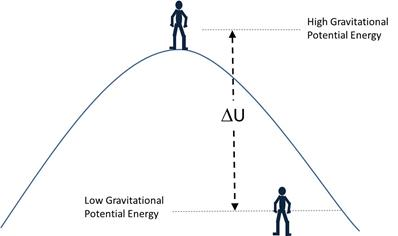
\includegraphics[width=3.3537in,height=1.9977in]{PH4CAU0F}
\end{figure}We have to do the same thing in
our electrical case. We need two \textquotedblleft
probes,\textquotedblright\ one placed at the high potential and one placed
at the low potential. For example, we could have the circuit that you see in
the next figure.\begin{figure}[h!]
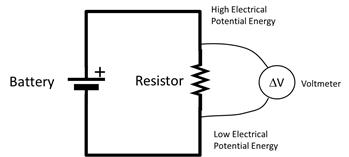
\includegraphics[width=2.9438in,height=1.3353in]{PH4CAU0G}
\end{figure}The positive end of the battery
is like the top of the hill. It provides a high electrical potential energy.
So we put one probe at the top of the \textquotedblleft
hill\textquotedblright\ or the plus side of the battery, and the other on
the bottom of the \textquotedblleft hill\textquotedblright\ or minus side of
the battery. The negative side of the battery provides a low electrical
potential energy. \emph{\ }With this we measure how high our potential
\textquotedblleft hill\textquotedblright\ is. The difference between these
two measurements is called \emph{voltage. }You should ask yourself
\textquotedblleft what would happen if you got the probes
backward?\textquotedblright\ 

In the next figure you can see how to actually perform this voltage
measurement with one of our meters.\begin{figure}[h!]
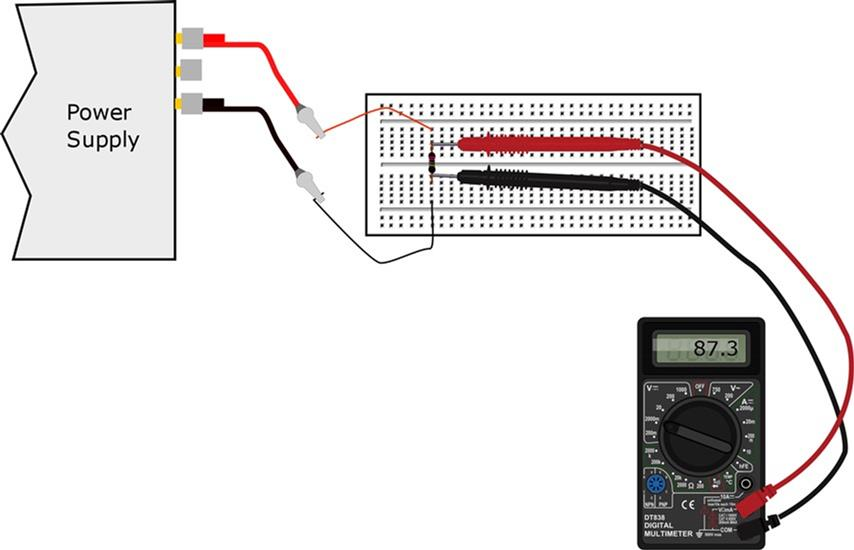
\includegraphics[width=5.5997in,height=3.614in]{PH4CAU0H}
\end{figure}

We say we measure voltage \textquotedblleft across\textquotedblright\ a
circuit element. This makes some sense if you consider that we very seldom
stand batteries up so their electric potential is greater in the same
direction as their gravitational potential. Batteries, resisters,
capacitors, etc., often lie down, and we measure \textquotedblleft
across\textquotedblright\ them by putting the positive probe on the high
potential side and the negative probe on the low potential side. Even though
the battery is lying down, we are still measuring a higher and lower
potential energy difference. Knowing a little about voltage, let's look at
our devices that produce voltages and then the devices that measure voltages.

\section{Experimental Hardware}

In today's lab we will study different hardware devices. A multimeter, power supply, a signal generator, and an oscilloscope. We will call these \textquotedblleft stand alone\textquotedblright\ instruments because they are independent boxes that do their job of measuring or generating signals without a computer connected to them. We will also look at the Arduino and how it can perform many of the same functions as the stand alone instruments. The power supply and the signal generator make voltage signals. The other devices measure them. Most of these devices are not to expensive to require students to purchase for just one lab. For this reason as a remote lab we will not be able to use them directly. You will likely encounter something like them at some point in your career so I've still included sections here for you to read. 

The Arduino acts as both a voltmeter and a power supply. It to can act as a stand alone instrument, but can also be used with a computer. For the first part of the class we will keep it connected to a computer to both tell it what to do and to read what it is measuring. Later labs we will explore using it without a computer. In this lab we will briefly explore how it can be used as a power supply and as a voltmeter in section \ref{ArduinoTour}. 

\subsection{Voltmeter/Multimeter}

Our first measurement device is voltmeter. It measures the electric potential (voltage) between its two leads (sometimes called \textquotedblleft probes\textquotedblright ). Here is a picture of one of our multi-meters set to measure voltage.

\begin{figure}[h!]
	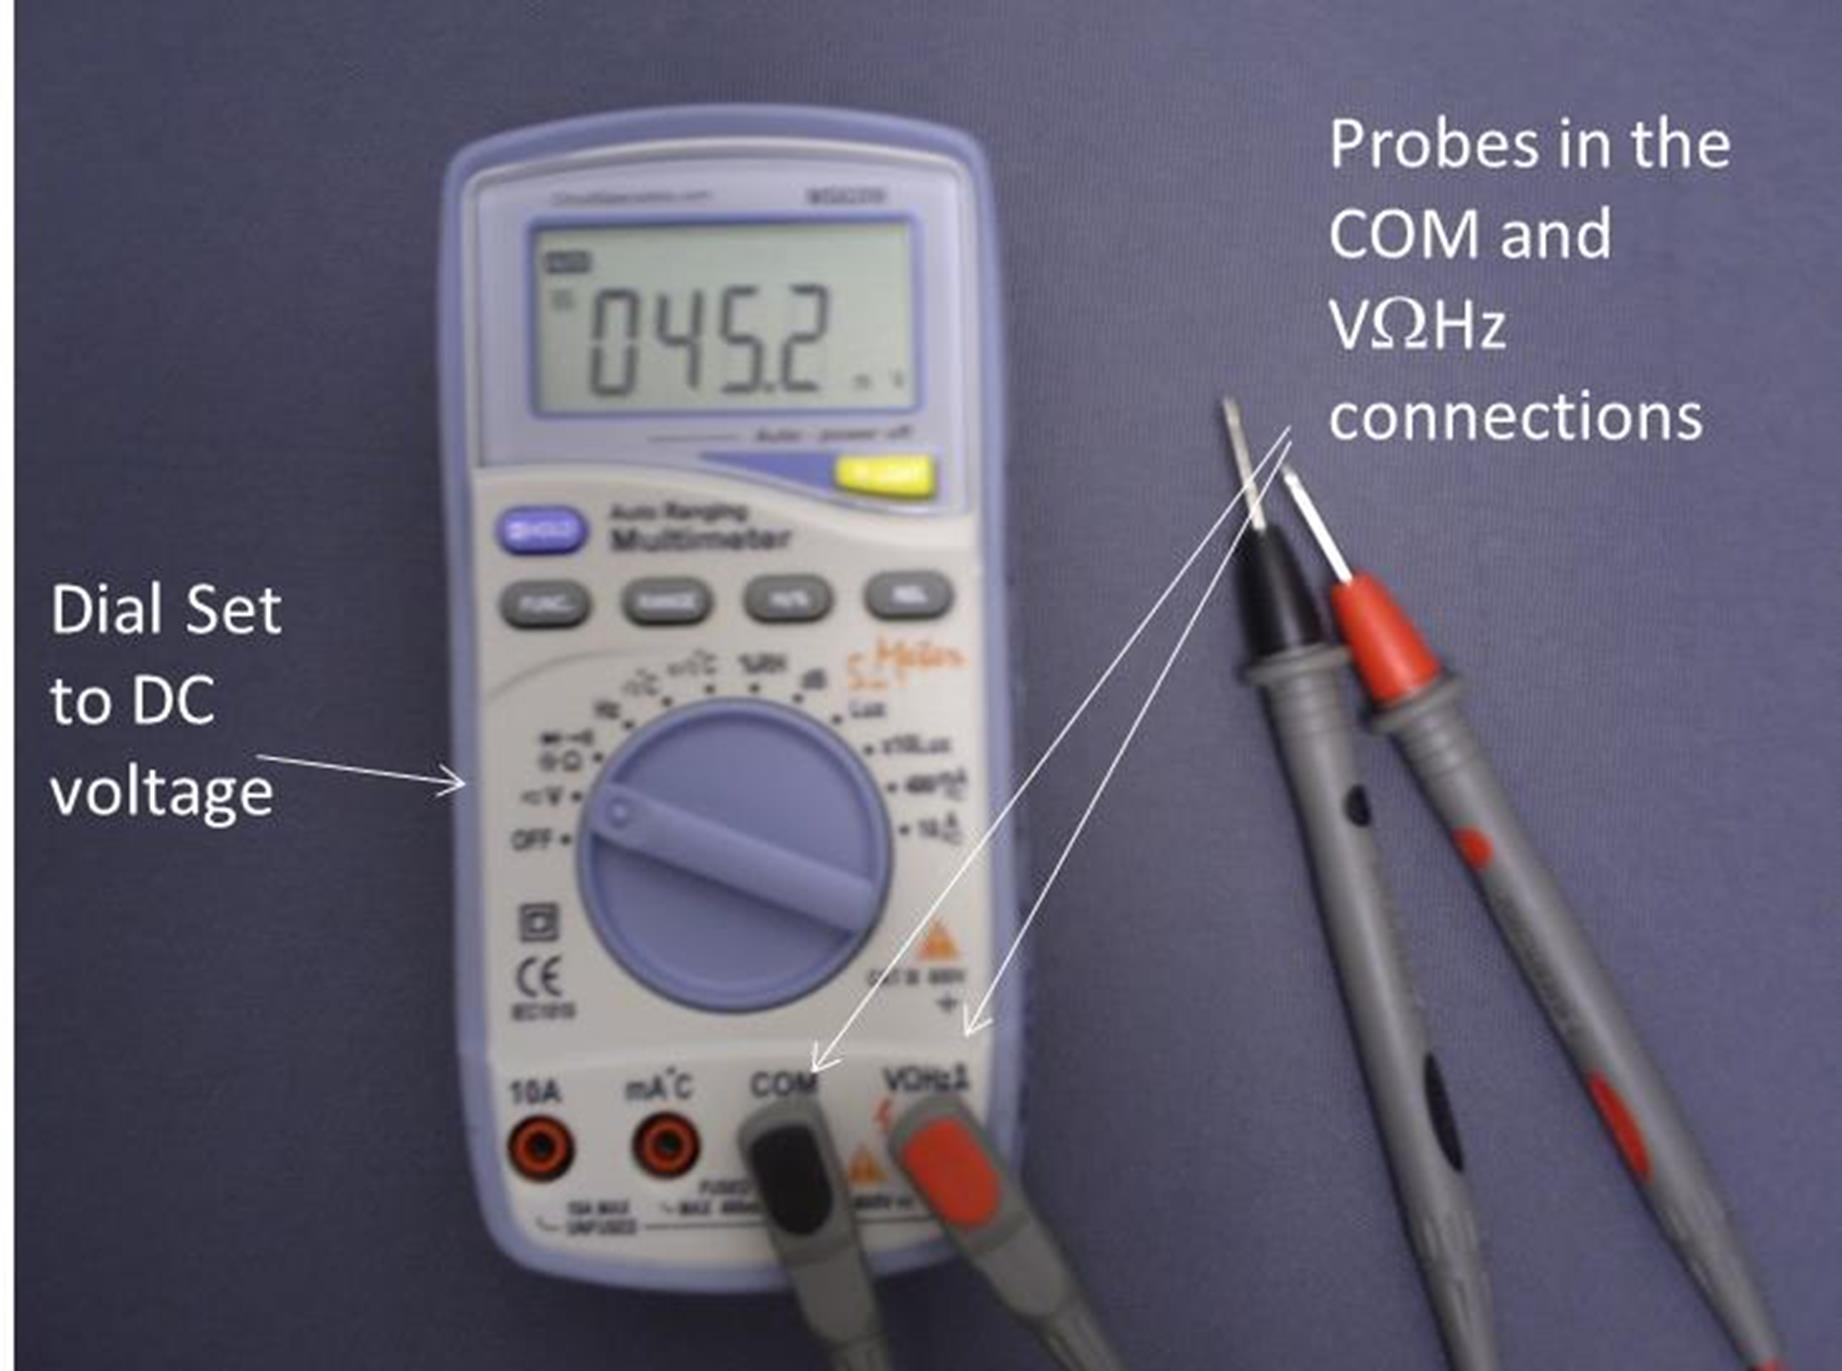
\includegraphics[width=3.116in,height=2.3266in]{PH4CAU0L}
\end{figure}

The display is set to read voltage by turning the dial to the $\unit{V}$ position. There are often two voltage settings. The one that has a wavy line next to it is alternating voltage. The one that has a straight line with three dots under it is the direct current (DC) voltage. These words might not mean much to you yet because you are just starting PH220. So for now, we will just use the DC voltage setting. As you learn more, we may use the alternating voltage setting. The leads (probes) should be connected to the COM (common) and $\unit{V}\unit{\Omega}\unit{Hz}$ connectors. Note that connecting your probe leads to the wrong position can blow the fuse (or worse) in your meter and make subsequent readings very wrong. You should make sure you don't do this, and watch to make sure someone else has not done this before you. If the meter seems crazy, it just may be. We have several different voltmeter models. Here is a picture of a different model.

\begin{figure}[h!]
	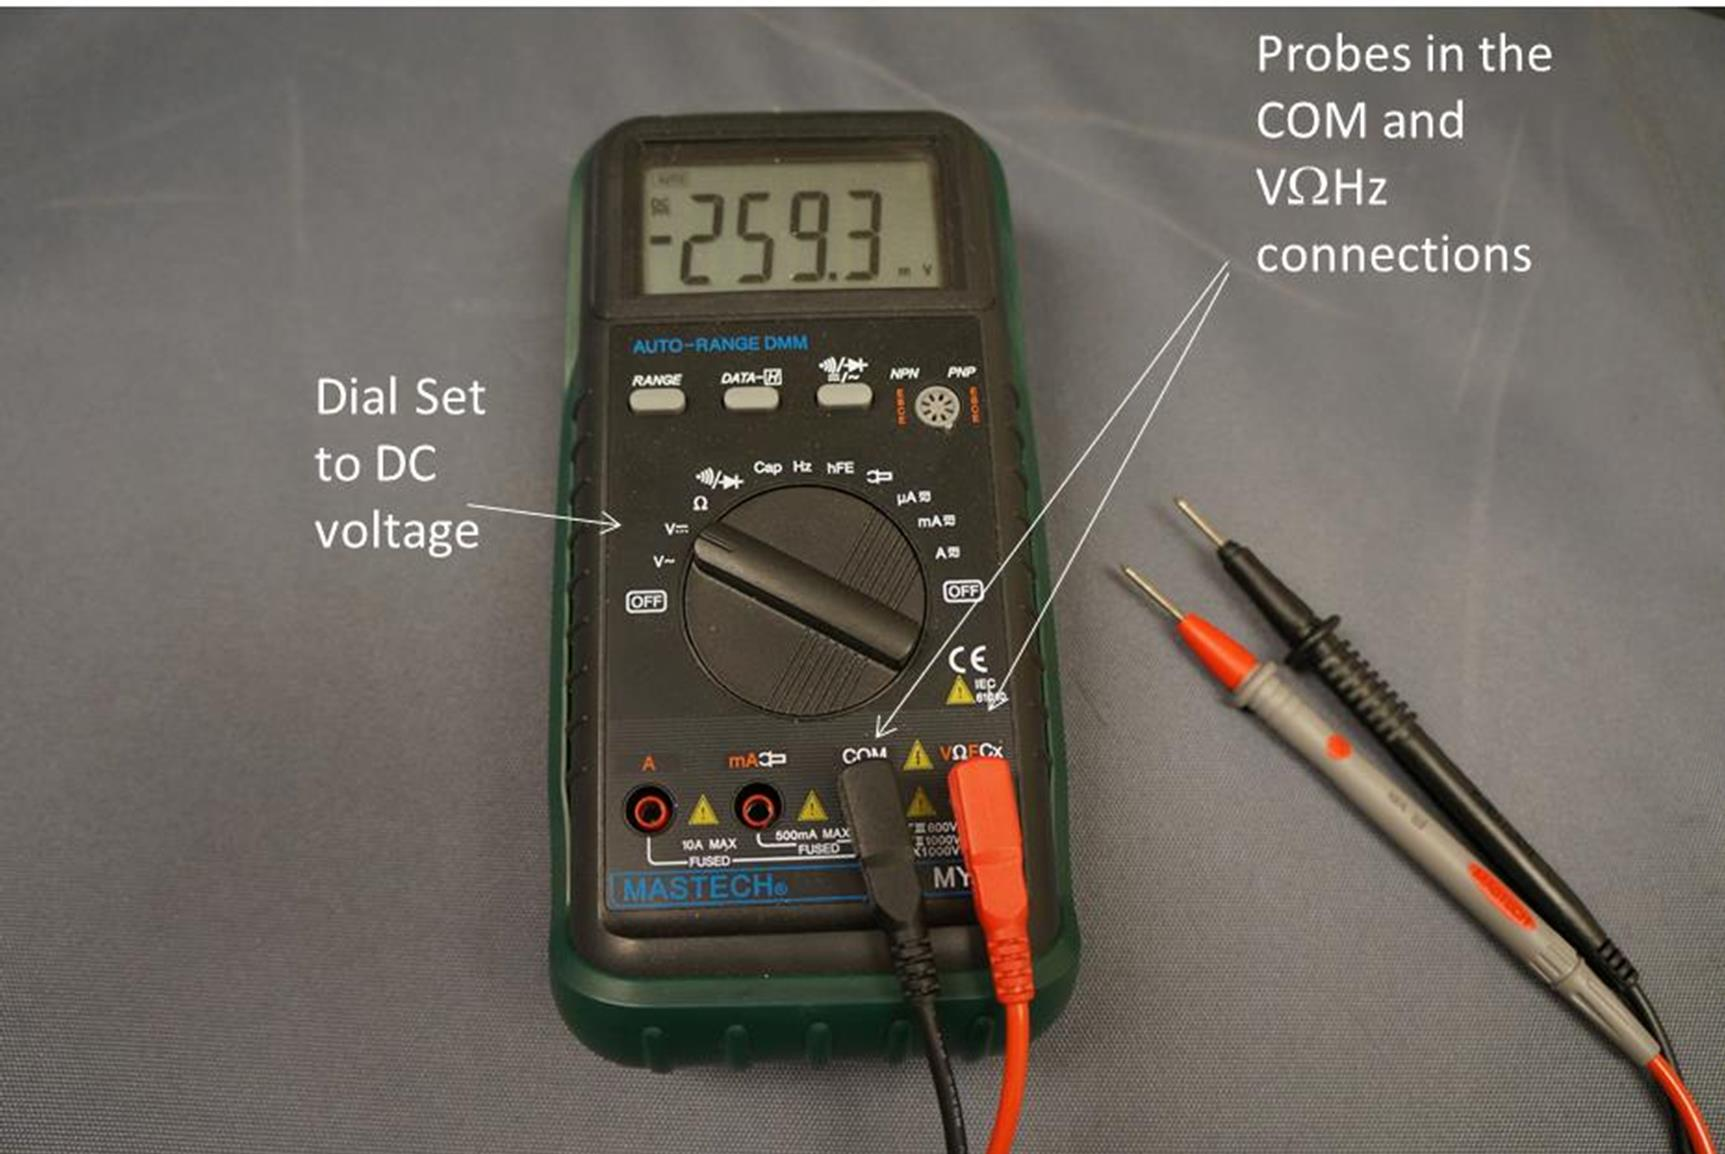
\includegraphics[width=2.9199in,height=1.962in]{PH4CAU0M}
\end{figure}

\begin{figure}[h!]
	\caption{AstroAI multimeter \label{AstroAI}}
	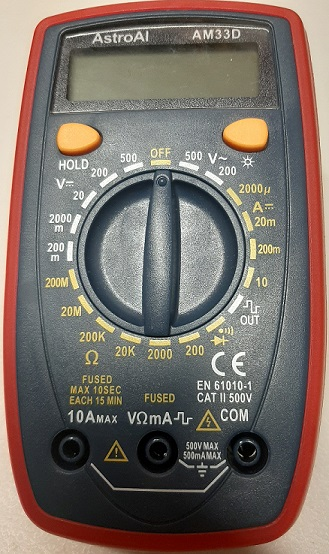
\includegraphics[width=2.5in]{AstroAIMultiMeter}
\end{figure}
\subsubsection{Signal Out}
You will notice that there are other settings besides volts. Our meters are all multi-meters. That means that they can measure more than one thing. We will use several of the settings throughout the semester. Take a look at the figure \ref{AstroAI} and also look at your own multimeter. One of the settings is unique to these multimeters.  It is white and can be found at about 4 o'clock on the dial. It has a square squiggle and simply says ``OUT''. This is an output signal like what you would see from a signal generator, see section \ref{siggen}. Only this is a fixed signal that oscillates at 50 times a second and goes from -5V to 5V. 

\subsubsection{Current}

Our multimeters have a current setting as well as a voltage setting. Current
is a flow of charge. This is like a water current, which is a flow of water.
Only we have a different thing flowing. We have a flow of charge. In the
wires in our Arduino, the moving charged things are (mostly) electrons. We
can write the flow of something as 
\begin{equation*}
I=\frac{\Delta Q}{\Delta t}
\end{equation*}%
where for us $\Delta Q$ is the amount of charge that has gone by in the time 
$\Delta t.$ Physicists use the letter $I$ for electrical current.

We should take a minute to think about what to expect when we allow charge
to flow. Think of a garden hose. If the hose is full of water, then when we
open the faucet, water immediately comes out. The water that leaves the
faucet is far from the open end of the hose, though. We have to wait for it
to travel the entire length of the hose. But we get water out of the hose
immediately! Why? \begin{figure}[h!]
	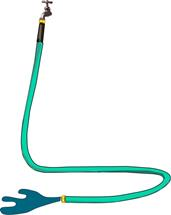
\includegraphics[width=1.4547in,height=1.8228in]{PH4CAU0V}
\end{figure}The new water coming in causes a
pressure change that is transmitted through the hose. The water at the open
end is pushed out. You can tell this is the case because the water
immediately leaving the hose is warm and tastes like plastic hose. After a
while, the water is colder and cleaner.

Current is a little bit like this. When we flip a light switch, the
electrons near the switch start to flow. But there are already free
electrons in the wire. These experience a push that makes the light turn on
almost instantly. But the electrons that turn on the light are not the ones
that just went through the switch.

\subsubsection{Measuring Current}
\label{MeasureA}
Because current is a flow, to measure current we must put a meter into that
flow. In a house, if you want to measure how much water is used, you connect
the pipe from the city water system to a meter. The water flows through the
meter and then goes into the pipe that brings water to the house. That way,
the meter can't miss any of the water (and the city can't miss any of your
payment!). The same is true for electrical current. To measure electrical
current, we need to remove part of our circuit, and replace it with the
meter to force the flow of electrical current to go through the meter. A
schematic diagram of this might look like this: \begin{figure}[h!]
	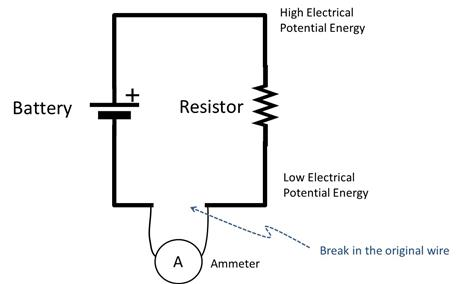
\includegraphics[width=3.8484in,height=%
	2.3981in]{PH4CAU0W}
\end{figure}In this diagram, you can see that
the electric current must go through the current meter. In fact, it couldn't
go anywhere else because part of the original circuit wire is missing. This
is just what we want. To actually perform this measurement with one of our
multimeters you could set up a circuit like the one in the following figure. 
\begin{figure}[h!]
	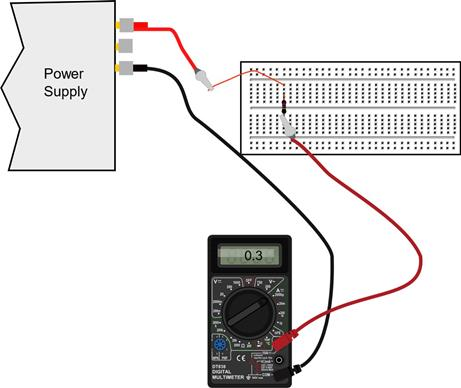
\includegraphics[width=3.8821in,height=3.2707in]{PH4CAU0X}
\end{figure}There is one more important thing
to do to make this work. We need to change the meter settings. And there are
two separate changes. The first is to switch the probe connections. One
probe stays in the COM or common connector, but the other needs to move to
the connector marked with an \textquotedblleft A.\textquotedblright\ Here is
an example showing the changes with two kinds of multimeters. \begin{figure}[h!]
	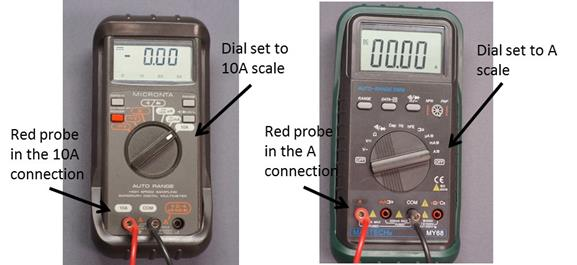
\includegraphics[width=%
	4.858in,height=2.2423in]{PH4CAU0Y}
\end{figure}The \textquotedblleft
A\textquotedblright\ stands for the standard unit of electrical current, the
Ampere or Amp. With the multimeter set up like this we would call it an 
\emph{ammeter}. Ammeters measure electrical current.



\subsection{Arduino as Power Supply and Voltmeter}
\label{ArduinoTour}
The Arduino is a little mini computer that can also measure voltage. It also has a power supply for limited electronics. Take a look at your Arduino and compare it to figure \ref{ArduinoLayOut}.
\begin{figure}[h!]
	\caption{Arduino lay out\label{ArduinoLayOut}}
	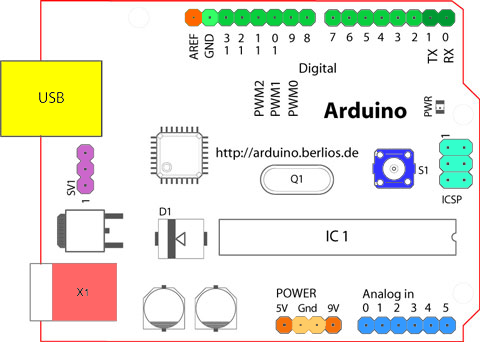
\includegraphics[width=3.116in]{arduino_board}
\end{figure}
Notice there are 3 main sets of pins (holes that you can put wires in). There are the digital pins, these are green in the figure. You used these last week to turn on and off a light. The blue ones are labeled Analog in. These are the same as a volt meter. Then there is the orange. These are kind of everything else. But we care most about the ones that are labeled with a V and Grd. These are voltage out and ground. 

The pins labeled 5V and 3.3V volts can be treated like a power supply. See section \ref{power}. But there are significant differences. The Arduino power pins can only output a single voltage, 3.3 or 5V. In addition they are very limited as to the amount of current they can supply at those voltages. They can only supply about 50mA. This is 60 times less than the desktop power supply described in a later section. 50mA is only enough to power a few LEDs. This will limit what we can do, but we should still be able to understand the physics. If you want to have more current you will need to get a different power supply. This could be as simple as a 9V battery, or maybe a plug in transformer from another device. This could come in useful when you are working on your student designed lab. For the other labs the 5V 50mA will be enough. 

The Analog in pins are also a lot like a voltmeter. But here again there are limitations. Thankfully there are also some really nice advantages as well. First the limitations. These pins can only measure voltages between 0V and 5V. The hand held voltmeter can go all the way from -500V to +500V. Also the analog pins can only measure to a certain precision. They can measure changes in voltage as small as about 4.9mV. This is significantly larger than the voltmeter.  Now for the good. Because these pins are attached to a mini computer the voltage can be measured over and over again. As often as about 10,000 times each second. Also we will see in later labs that these values can then be stored on a SD card to look at later. You can't do that with the hand held voltmeter! This is instead similar to a stand alone oscilloscope, see section \ref{oscilly}


\subsection{Power Supply}
\label{power}
A power supply is like an adjustable battery. Batteries have fixed voltages.
But a power supply may have an adjustable voltage. \begin{figure}[h!]
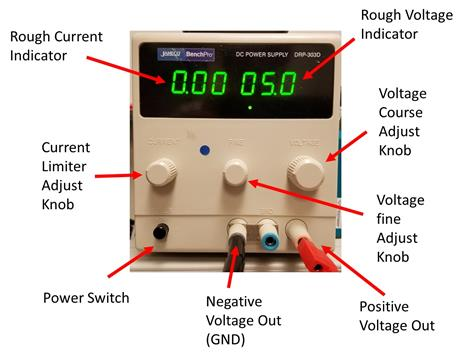
\includegraphics[width=3.9237in,height=%
3.0191in]{PH4CAU0I}
\end{figure}Usually a power supply takes
electrical energy from the wall outlets and converts that energy into the
specific voltage range that we want for our experiment. So it is like a
battery, but must be plugged into the wall. Our power supplies are designed
to keep us safe. They are current limited, meaning that they try not to give
too much charge flowing through our wires. Sometimes this is a problem
because they are too limited. There is a current limiting knob that you can
turn to allow a little more current. Be careful when you use this. The
voltage may jump wildly when you turn the current knob! It is best to turn
all the knobs down as low as they will go before you turn on the power
supply. Then, after turning on the power supply, increase the current knob
about half a turn and then slowly turn the voltage knob up to your desired
voltage. If the voltage stops increasing, turn the voltage knob back down a
bit, and turn up your current limiter knob some more. Then try your voltage
knob again.

Some of our electrical devices are quite delicate, and will literally burn
up if you apply too much current or voltage. In today's lab, we will
practice using our power supply so we are prepared when the delicate
components come out later.

\subsection{Signal Generator}
\label{siggen}
\begin{figure}[h!]
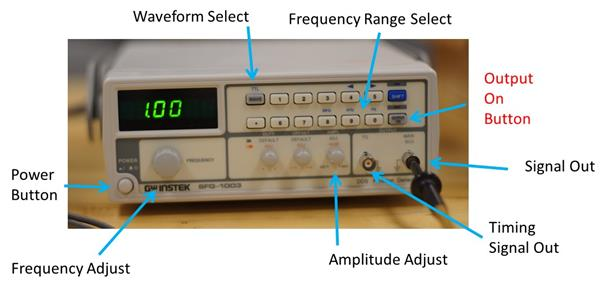
\includegraphics[width=5.093in,height=2.4348in]{PH4CAU0J}
\end{figure}The signal generator is a fancy
power supply. It makes changing voltages. It can make voltages in sine,
square, and triangle patterns. These time-varying signals have a maximum
voltage (called the amplitude) . We will use both the wave output and a
timing signal that the wave generator creates. Each has their own Bayonet
Neill--Concelman connector (usually just called a BNC connector) on the
front of the signal generator. You will need a cable with BNC connectors on
one end (and maybe alligator clips on the other end) to use this device.
There is an amplitude knob on the front of the signal generator. Because the
signal generator makes a voltage that changes in time, the amplitude of the
signal must be in voltage units. We should be careful not to set the signal
amplitude (voltage) too high or we run the risk of destroying our measuring
devices. Again turn the amplitude (voltage) down before you connect the box
to our electrical components. Then turn up the voltage to what you want in a
safe way.

There are frequency range buttons (using the shift button) near the middle
of the device panel. To change the frequency, you use the shift and range
buttons to set which digit you are adjusting, then turn the frequency knob
to make the change. An annoying feature of our frequency generators is that
you must push the \textquotedblleft output on\textquotedblright\ button or
they don't output a signal. When everything is set up right, we get a sine
wave (or square wave, or triangle wave) out. Here is a signal from the
signal generator displayed on one of our measuring devices, the
oscilloscope. \begin{figure}[h!]
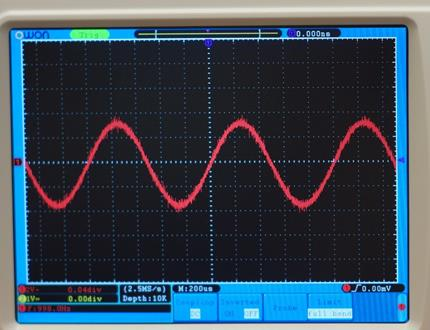
\includegraphics[width=3.6262in,height=2.7882in]{PH4CAU0K}
\end{figure}

Of course, simple batteries are sources of voltage, and so are many other
things.



\subsection{Oscilloscope}
\label{oscilly}
Our next device, the oscilloscope, is just a fancy voltmeter. Unlike the
multimeter, it usually just measures voltage. But it does it with flare!

The oscilloscope can measure changing voltages very accurately and usually
has a way to graph the changing voltage. The standard is a voltage vs. time
graph. A sinusoidally varying voltage should look something like this when
plotted. \begin{figure}[h!]
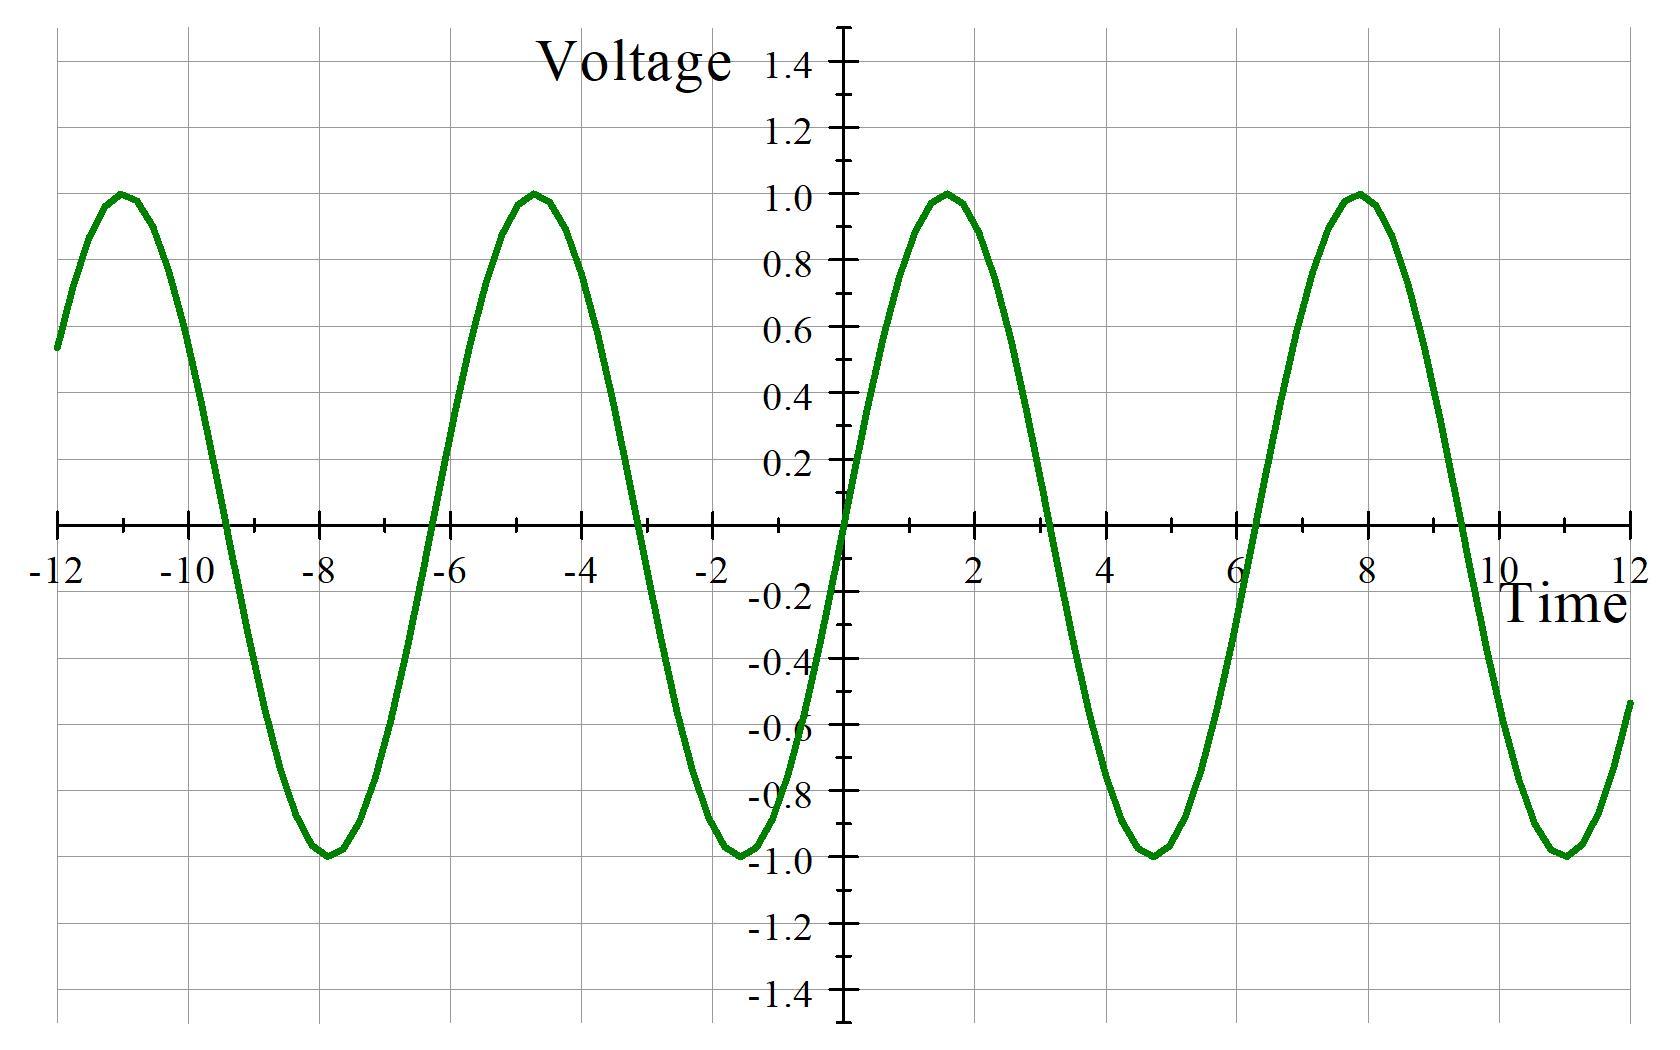
\includegraphics[width=4.4997in,height=3.0007in]{PH4CAU0N}
\end{figure}And that is what our oscilloscope
does. We should see something like this on the oscilloscope screen. From our
discussion of the signal generator, you know that this is just what we see.%
\begin{figure}[h!]
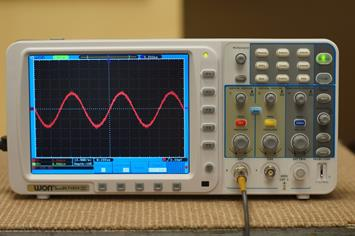
\includegraphics[width=2.998in,height=1.9993in]{PH4CAU0O}
\end{figure}

If the changing voltage is periodic, the oscilloscope has a way to use this
fact to stabilize the graph so you can see the details more clearly. This
stabilization is called \textquotedblleft triggering\textquotedblright\ and
on our oscilloscopes there are buttons and knobs on the right hand side of
the oscilloscope that adjust the triggering to make the graph more stable
(or less stable). The photograph of the sine wave above was taken by
stabilizing a sine wave from our signal generator. The oscilloscope starts
plotting at the same part of the wave each time, so the periodic signal
seems to stand still. To do this we must \textquotedblleft
trigger\textquotedblright\ the graph at some good starting point. Our
oscilloscopes have a build-in circuit that can watch for the same part of a
signal and start the graph in the same place each time. One of the knobs
adjusts the trigger point. \begin{figure}[h!]
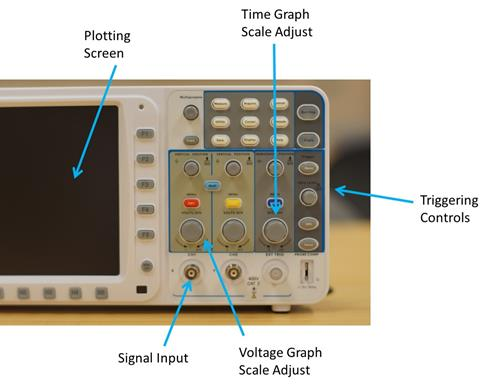
\includegraphics[width=4.23in,height=3.2659in]{PH4CAU0P}
\end{figure}The other controls adjust the
horizontal and vertical axes. The vertical axis is voltage, and the voltage
axis control is next to the signal input toward the bottom middle of the
front panel. To the right of this is the horizontal axis control, which is
time. You can choose how many volts per division with one knob and how many
seconds (or fractions of seconds) per division you have on your graph with
another knob. In the next figure you can see a signal on the oscilloscope
screen. \begin{figure}[h!]
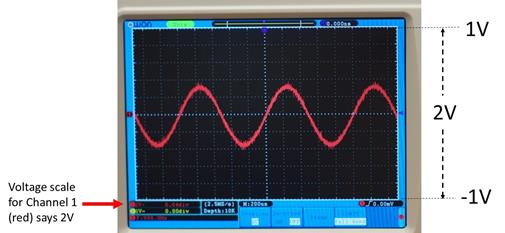
\includegraphics[width=4.2505in,height=1.9718in]{PH4CAU0Q}
\end{figure}In the bottom left-hand corner
there is a red dot and a voltage given. This is the voltage displayed across
the whole screen. Since when this photo was take the voltage knob was set to 
$2\unit{V}$, this means that the bottom of the screen represents $-1\unit{V}$
and the top of the screen represents $+1\unit{V}.$ \begin{figure}[h!]
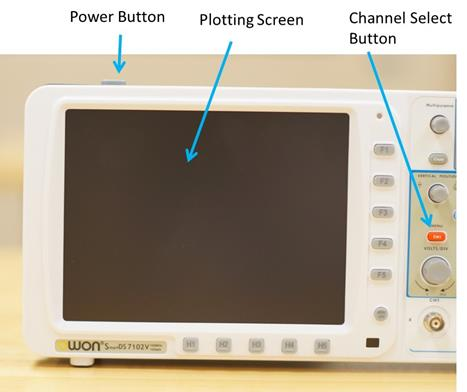
\includegraphics[width=3.9364in,height=%
3.3076in]{PH4CAU0R}
\end{figure}

There are two signal inputs because our oscilloscopes can look at two
different voltage signals at the same time. Each signal input is called a
\textquotedblleft channel.\textquotedblright\ Each channel has it's own
voltage scale knob and voltage scale indicator in the bottom left-hand
corner. They share the same time scale.

The channel inputs each have a BNC connector. We use oscilloscope probes
connected to these connectors. Notice that since there are two channels, an
oscilloscope can measure two voltages at once. But that means we may need
two probes!

To check that our oscilloscope is working correctly we can measure a known
voltage, say, the voltage of a regular battery.

\begin{figure}[h!]
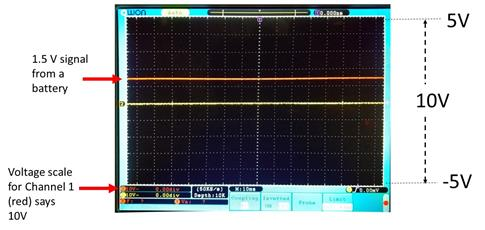
\includegraphics[width=4.0836in,height=1.9458in]{PH4CAU0S}
\end{figure}Notice that I changed the voltage
scale knob position so that now the oscilloscope screen has a $10\unit{V}$
total potential change. That means that we have $5\unit{V}$ at the top of
the screen and $-5\unit{V}$ at the bottom of the screen. The screen is
divided into little boxes. There are five rows of boxes from the bottom to
the top of the screen. Each box represents $1/10$ of the total voltage.
Since we have $\Delta V=10\unit{V},$ each box represents $\Delta V=1\unit{V}%
. $ So our battery voltage should give us one and a half boxes. And that is
just what we got.

But sometimes the oscilloscope does not get the right voltage. If this
happens we need to calibrate the oscilloscope. Every time we use an
Oscilloscope it is a good idea to check it to make sure it working well. Our
oscilloscopes have a test voltage to use just for this purpose.

\begin{figure}[h!]
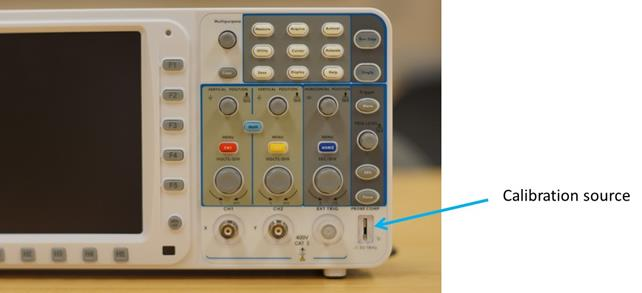
\includegraphics[width=5.3982in,height=2.4742in]{PH4CAU0T}
\end{figure}

The calibration source makes a $5\unit{V}$ square wave (try it to see what
that looks like!). If we use this calibration source we should get something
like what you see in the next figure. \begin{figure}[h!]
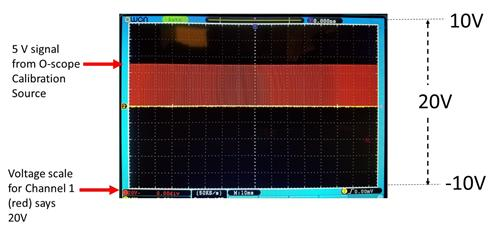
\includegraphics[width=4.2004in,height=1.9623in]{PH4CAU0U}
\end{figure}If you don't get $5\unit{V},$
then some thing is wrong and you will need to go through the oscilloscope's
calibration procedure. That is in the oscilloscope manual and you can find
the manual on-line.








\section{Lab Assignment}


%\subsection{Practice Measurements}

\subsection{Use a Multimeter}

\begin{enumerate}
	\item Measure the voltage of a 9-V battery with a voltmeter. Report the
	value you get from the measurement and the uncertainty.
	
	\item Set up the circuit described in section (\ref{Voltage Measurement with
		Meter}). The figure is repeated below. Measure the voltage with a
	multimeter. Use the Arduino 5V power supply and ground. Do you measure exactly 5V?
	\begin{figure}[h!]
		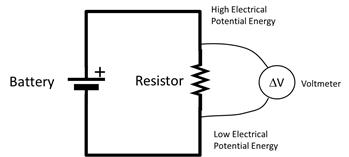
\includegraphics[width=2.9438in,height=1.3353in]{PH4CAU1G}
	\end{figure}
	
	\item Modify your circuit to measure current as described in section (\ref{MeasureA}) and change the settings of your multimeter so that you measure the current in the circuit. Connecting the multimeter probes can be problematic in this situation because the connections themselves can act like resistors. Don't worry to much about this during this lab. We will explore this issue more in the next lab. For now I just want you to get experience using the multimeter to measure current. 
\end{enumerate}


\subsection{Simple Arduino Voltmeter}

\begin{enumerate}
	\item Put the circuit back together to measure voltage again.
	 \begin{figure}[h!]
		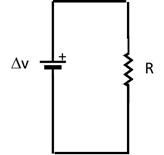
\includegraphics[width=1.3932in,height=1.3188in]{PH4CAU1Z}
	\end{figure}(see section (\ref{Voltage
		Measurement with Meter}). \begin{figure}[h!]
		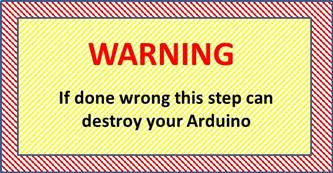
\includegraphics[width=1.8507in,height=0.9677in]{PH4CAU20}
	\end{figure}This time write the simple voltmeter sketch, wire it up, and measure the voltage across the resistor
	using our Arduino and the serial monitor. Be careful trying to measure any voltage out side the $0$ to $5\unit{V}$ range could damage your Arduino!
	
	%\item Calculate the uncertainty due to quantization error for your Arduino	simple voltmeter
	
	%\item Compare your calculated uncertainty to the measured uncertainty that you see in your device output. (This is tricky, does the power supply give a truly constant voltage?)


\end{enumerate}












\subsection{Seeing the data}

Once the code is compiled and uploaded, the Arduino will send data to the
serial port. The serial monitor can display the data. The serial monitor is
found under the Arduino Software Tools menu. See figure \ref{tools}

\begin{figure}[h!]
	\caption{Arduino IDE Tools\label{tools}}
	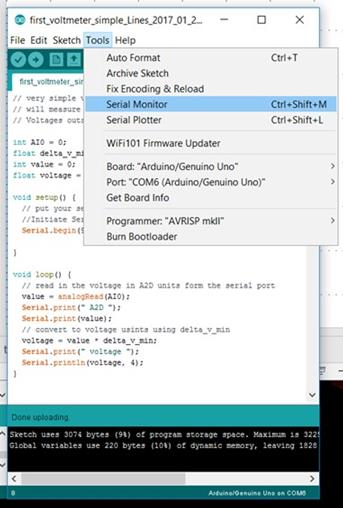
\includegraphics[width=2.0807in,height=3.0744in]{PH4CAU1P}
\end{figure}
You should then see something like figure \ref{monitor}

\begin{figure}[h!]
	\caption{Arduino Serial Monitor\label{monitor}}
	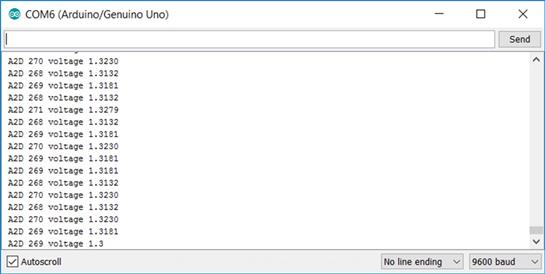
\includegraphics[width=4.5861in,height=2.3151in]{PH4CAU1Q}
\end{figure}

The Arduino Software can also plot the data from the serial port. Here is a
plot of the same data that we saw on the serial monitor. 
\begin{figure}[h!]
	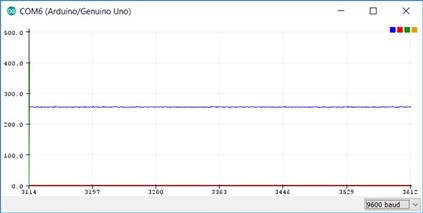
\includegraphics[width=%
	3.563in,height=1.8049in]{PH4CAU1R}
\end{figure}
Notice that it plotted our voltage values and it also plotted our ADC values. This makes the voltage
values hard to see. We could fix this by commenting out the lines that print
the ADC values (putting \textquotedblleft //\textquotedblright\ at the
beginning of the line). Then those lines won't be executed by the Arduino.
Then we get just the voltage. 
\begin{figure}[h!]
	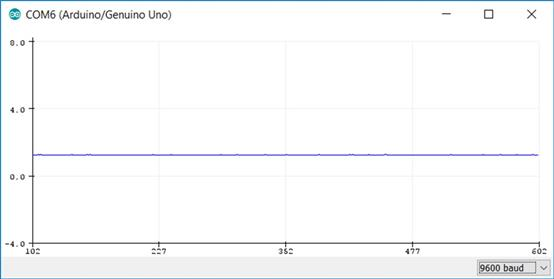
\includegraphics[width=3.2578in,height=1.6475in]{PH4CAU1S}
\end{figure}
Notice that the horizontal axis
is not exactly time. It is just the data point number. We could convert this
to time with some calculation if we know how often the Arduino sends us a
data point. I will leave this as an exercise.




\subsection{Measuring a Changing Voltage}
Using the same code measure the voltage from the "OUT" on your AstroAI multimeter. In other words conect the probes from the multimeter to the ground and one of the Analog in pins on the Arduino. Be sure the multimeter dial is set to the "OUT" position. Then run the voltage measuring code on your Arduino. This time instead of opening the "Serial Monitor" try looking at the "Serial Plotter".  What do you see? Try changing the amount of time the program waits between loops. This is done by adding the commend "delay(3)". The 3 is the amount of milliseconds that the Arduino will wait before continuing on with the loop. Change the time. Try 10, 20, 21, 40, and others. How does that affect what you see and why? Remember the voltage signal from the multimeter is -5$\unit{V}$ to +5$\unit{V}$ that cycles 50 times every second (50$\unit{Hz}$).



	
	
	
	
\subsection{Voltage Divider}
	
	\begin{enumerate}
		\item Build the voltage divider using two resistors as shown in figure \ref{VoltageDivider}. You will have to think about which resistors from our set will work best. Discuss this with your group, or have group members try the calculations with different combinations. Use the 5$\unit{V}$ power from the Arduino for your power supply
		\begin{figure}[h!]
			\caption{Voltage Divider\label{VoltageDivider}}
			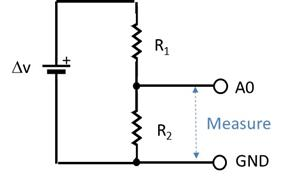
\includegraphics[width=2.3851in,height=1.5469in]{PH4CAU22}
		\end{figure}
		
		\item Use a multimeter to verify that the output of the voltage divider (the voltage between the resistors) is at least roughly what you would expect.  Try switching the power voltage to the 3.3$\unit{V}$ and check again with the multimeter what the voltage is between the resistors.
		
%		\item \begin{figure}[h!]
%			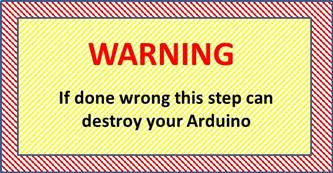
\includegraphics[width=1.8507in,height=0.9677in]{PH4CAU21}
%		\end{figure}
		
		\item Write the sketch (the code) and then hook the output of your voltage divider to the A0 pin and the other side of $ R_{2} $ to a GND pin.

		Your Arduino voltmeter should now be set up. Compile and load the sketch and use the Serial Plotter to watch the voltage values as you change the power supply from $5$ to $3.3\unit{V}$. 
		
		%\item What is the quantization error for this voltmeter? Check to see if this matches your values on the serial monitor.
		
		%\item Design a voltage divider that will allow the full $0$ to $30\unit{V}$ range of our power supply to be measured using the Arduino's $0$ to $5\unit{V}$ analog input. What would the quantization error be for this new circuit?
		
		\item The analog in pins can only measure voltages less than 5$\unit{V}$ and greater than 0$\unit{V}$. Can you think of a way you could measure voltages higher than 5$\unit{V}$ with the Arduino?
		
	\end{enumerate}






%TCIMACRO{\TeXButton{\vspace*{\fill}}{\vspace*{\fill}}}%
%BeginExpansion
\vspace*{\fill}%
%EndExpansion
\pagebreak


%\section{Extending our voltmeter with a voltage divider\label{Voltmeter with
%		Voltage Divider}}
%
%This Arduino-based voltmeter that we have built is great, but will only let
%us measure voltages in the range $0$ to $5\unit{V}.$ That seems a little
%restrictive. We would like to extend our voltmeter to a larger range, say, $%
%0 $ to $20\unit{V}.$ To do this, we will need to add some electronic
%components and think about what we have learned about voltage, resistance,
%and current. Let's consider this circuit.\begin{figure}[h!]
%	\includegraphics[width=1.3932in,height=1.3188in]{PH4CAU1T}
%\end{figure}We have a battery, That will make
%the current flow much like a pump makes water move through pipes.
%
%\begin{figure}[h!]
%	\includegraphics[width=4.2004in,height=2.3229in]{PH4CAU1U}
%\end{figure}The water in a pipe system gains
%potential energy as it moves up. In our circuit we will find that electric
%charge gains potential energy as we move it across a battery. Then the
%charge will move down the wire like water moves down a pipe until it is out
%of potential energy. Notice that the water in a pipe system will lose all
%the potential energy that it gained when the pump raised it to the upper
%tank (see previous figure). That is true of electric charge too. The
%electric current travels from the battery through the resistor, but in doing
%so it loses all the potential energy that the battery gave it by the time it
%returns to the battery.
%
%Now suppose we have two resistors in a circuit. \begin{figure}[h!]
%	\includegraphics[width=1.7279in,height=%
%	1.5947in]{PH4CAU1V}
%\end{figure}
%
%Our water analogy can still help us understand what will happen. Suppose
%that we have two turbines in our pipe system. \begin{figure}[h!]
%	\includegraphics[width=3.5985in,height=%
%	1.9934in]{PH4CAU1W}
%\end{figure}The water leaves the high
%potential energy part of the pump, and is put to work turning the first
%turbine. The resistance of the turbine will slow the water current. So when
%the water leaves the turbine, it will have lost some potential energy. Since
%we have a second turbine the current will again be slowed and more potential
%energy will be lost. How much potential energy do we lose as the water
%falls? All of the potential energy that the pump gave it! We must end up
%with the water at the bottom back at the low potential energy. We will find
%this to be true for our electric circuit as well. We will loose some
%potential energy as the electrical energy \textquotedblleft
%falls\textquotedblright\ from the high electric potential \textquotedblleft
%down\textquotedblright\ the first resistor. After the second resistor, we
%can guess that we must be back at the low electric potential we started with.
%
%\begin{figure}[h!]
%	\includegraphics[width=1.7279in,height=1.5947in]{PH4CAU1X}
%\end{figure}We know that electric potential
%is a potential energy per unit charge. And energies just add up. If 
%\begin{equation*}
%\Delta V=RI
%\end{equation*}%
%is satisfied, then we would expect that adding two resistors would just
%linearly add the effects of the two resistors together%
%\begin{eqnarray*}
%	\Delta V_{total} &=&\Delta V_{1}+\Delta V_{2} \\
%	&=&R_{1}I+R_{2}I
%\end{eqnarray*}%
%Note that the same current must flow through each of the resistors, since
%the current leaving $R_{1}$ is the current flowing into $R_{2}.$ Then 
%\begin{equation*}
%\Delta V_{total}=\left( R_{1}+R_{2}\right) I
%\end{equation*}%
%Our current will be 
%\begin{equation*}
%I=\frac{\Delta V_{total}}{R_{1}+R_{2}}
%\end{equation*}
%
%But suppose we measure the potential change across just resistor $R_{2}.$ 
%\begin{figure}[h!]
%	\includegraphics[width=1.7625in,height=1.0421in]{PH4CAU1Y}
%\end{figure}what would we expect to get? We
%lost voltage across both $\Delta V_{1}$ and $\Delta V_{2}$ so 
%\begin{equation*}
%\Delta V_{total}=\Delta V_{1}+\Delta V_{2}
%\end{equation*}%
%because we must loose all the $\Delta V_{total}$ given to the current by the
%battery. And 
%\begin{equation*}
%\Delta V_{2}=IR_{2}
%\end{equation*}%
%from Ohm's law. So
%
%\begin{equation*}
%\Delta V_{2}=\left( \frac{\Delta V_{total}}{R_{1}+R_{2}}\right) R_{2}
%\end{equation*}%
%This is only part of the total voltage. And if we have two different
%resistors so that $R_{1}\neq R_{2}$ then we can choose for $\Delta V_{2}$ to
%be nearly as much as $\Delta V_{total}$ or nearly as little as $0$ by
%carefully choosing our two resistances. We call a set of two resistors like
%this a \textquotedblleft voltage divider\textquotedblright\ because it
%divides the battery voltage between the two resistors. If $R_{1}$ is bigger
%than $R_{2}$ then $\Delta V_{1}$ is bigger than $\Delta V_{2}.$
%
%Remember that the input can only withstand $0$ to $5\unit{V}.$ More than
%that can destroy the board! But we want to measure a voltage that varies
%from $0$ to $20\unit{V}.$ We now have a way to do this. We will use a
%voltage divider. The voltage across both resistors will be as much as $20%
%\unit{V},$ but we will measure the voltage across only one of the resistors.
%And we will choose our resistor so that when the total voltage is $20\unit{V}
%$ but the voltage across our resistor is $5\unit{V}$ (or less). Since we
%will know the resistances, we can use a little math to calculate what the
%total voltage was using the voltage measurement from just one of the
%resistors.
%
%This is like what we did to measure current last lab. We used a voltmeter
%and a resistor and some math to make an ammeter. Today we will use two
%resistors, our Arduino voltmeter, and some math to make a new voltmeter that
%can measure higher voltages. We just need to choose our resistors so that we
%map our $0$ to $20\unit{V}$ to $0$ to $5\unit{V}.$ Once choice might be 
%\begin{eqnarray*}
%	R_{1} &=&40\unit{k%
%		%TCIMACRO{\U{3a9}}%
%		%BeginExpansion
%		\Omega%
%		%EndExpansion
%	} \\
%	R_{2} &=&10\unit{k%
%		%TCIMACRO{\U{3a9}}%
%		%BeginExpansion
%		\Omega%
%		%EndExpansion
%	}
%\end{eqnarray*}%
%Let's try it. We would get%
%\begin{eqnarray*}
%	\Delta V_{2\max } &=&\left( \frac{20\unit{V}}{40\unit{k%
%			%TCIMACRO{\U{3a9}}%
%			%BeginExpansion
%			\Omega%
%			%EndExpansion
%		}+10\unit{k%
%			%TCIMACRO{\U{3a9}}%
%			%BeginExpansion
%			\Omega%
%			%EndExpansion
%	}}\right) \left( 10\unit{k%
%		%TCIMACRO{\U{3a9}}%
%		%BeginExpansion
%		\Omega%
%		%EndExpansion
%	}\right) \\
%	&=&4.0\unit{V}
%\end{eqnarray*}%
%when $\Delta V_{total}=20\unit{V}$ and 
%\begin{eqnarray*}
%	\Delta V_{2\min } &=&\left( \frac{0\unit{V}}{40\unit{k%
%			%TCIMACRO{\U{3a9}}%
%			%BeginExpansion
%			\Omega%
%			%EndExpansion
%		}+10\unit{k%
%			%TCIMACRO{\U{3a9}}%
%			%BeginExpansion
%			\Omega%
%			%EndExpansion
%	}}\right) \left( 10\unit{k%
%		%TCIMACRO{\U{3a9}}%
%		%BeginExpansion
%		\Omega%
%		%EndExpansion
%	}\right) \\
%	&=&0\unit{V}
%\end{eqnarray*}%
%when $\Delta V_{total}=0\unit{V}.$ Notice that this really didn't work. We
%only got a maximum voltage of $4\unit{V}.$ But this gives us a margin of
%safety. If we give our Arduino more than $5\unit{V}$ we can burn it up. If
%we plan our circuit so we don't get to close to $5\unit{V}$ we are safer. So
%this set of resisters is not a terrible choice.
%
%To report out our voltage we need to do this conversion backwards. Say we
%have $\Delta V_{total}=10\unit{V}$ that we are measuring with our new
%instrument. Then 
%\begin{eqnarray*}
%	\Delta V_{2} &=&\left( \frac{10\unit{V}}{40\unit{k%
%			%TCIMACRO{\U{3a9}}%
%			%BeginExpansion
%			\Omega%
%			%EndExpansion
%		}+10\unit{k%
%			%TCIMACRO{\U{3a9}}%
%			%BeginExpansion
%			\Omega%
%			%EndExpansion
%	}}\right) \left( 10\unit{k%
%		%TCIMACRO{\U{3a9}}%
%		%BeginExpansion
%		\Omega%
%		%EndExpansion
%	}\right) \\
%	&=&2\unit{V}
%\end{eqnarray*}
%
%The $2\unit{V}$ is what we actually measure at the A0 input. But we know
%that this represents $10\unit{V}$ across both resistors, so we want the
%Arduino program to print out $10\unit{V}.$ So we report%
%\begin{equation*}
%\Delta V_{reported}=\frac{\Delta V_{2}}{R_{2}}\left( R_{1}+R_{2}\right)
%\end{equation*}%
%or for our case, since we measured $2\unit{V}$ across our resistor,%
%\begin{equation*}
%10\unit{V}=\frac{2\unit{V}}{\left( 10\unit{k%
%		%TCIMACRO{\U{3a9}}%
%		%BeginExpansion
%		\Omega%
%		%EndExpansion
%	}\right) }\left( 40\unit{k%
%	%TCIMACRO{\U{3a9}}%
%	%BeginExpansion
%	\Omega%
%	%EndExpansion
%}+10\unit{k%
%	%TCIMACRO{\U{3a9}}%
%	%BeginExpansion
%	\Omega%
%	%EndExpansion
%}\right)
%\end{equation*}%
%We will have to write this math in our code. There is a further
%complication. The Arduino A0 input is giving us a number that represents $0$
%to $4\unit{V}$ for our setup. But that is not what we see on the serial
%port. We see a number from 0 to 1024. We know the $1024$ represents $5\unit{V%
%}$ and the $0$ represents $0\unit{V}.$ So we need to multiply the number
%that comes from our Arduino by $\delta V=4.9\unit{mV}$ once again to get our
%Arduino output into voltage units. So our reported voltage equation is
%something like this. 
%\begin{equation*}
%\Delta V_{reported}=A2D\times \delta V_{2}\times \frac{1}{R_{2}}\left(
%R_{1}+R_{2}\right)
%\end{equation*}
%
%All this calculation to get our reported voltage must do something to our
%measurement uncertainty. We could do our usual math to find the reported
%uncertainty, but instead, let's think. Every small voltage $\Delta V_{2}$
%would be multiplied by $\left( \frac{1}{R_{2}}\left( R_{1}+R_{2}\right)
%\right) $ to map it into our original $0\unit{V}$ to $20\unit{V}$ range.
%That should work for our smallest voltage that we can detect, namely $\delta
%V=4.9\unit{mV}.$ That is the smallest value $\Delta V_{2}$ could have. So in
%our $0\unit{V}$ to $20\unit{V}$ range the smallest value this can map to is 
%\begin{equation*}
%\delta V_{reported}=\left( \delta V\right) \left( \frac{1}{R_{2}}\left(
%R_{1}+R_{2}\right) \right)
%\end{equation*}%
%The first term in parenthesis is essentially $1$ digitizer unit multiplied
%by $\Delta V_{2}$ and the second term in parenthesis converts the $\Delta
%V_{2}$ value into actual volts measured across both resistors.
%
%The quantity $\delta V_{reported}$ gives us our quantization error value for
%our new instrument. Our output will be in multiples of 
%\begin{equation*}
%V_{reported}=n\times \delta V_{reported}
%\end{equation*}%
%Putting in numbers gives 
%\begin{eqnarray*}
%	\delta V_{reported} &=&\left( 4.\,\allowbreak 884\times 10^{-3}\unit{V}%
%	\right) \left( \frac{1}{10\unit{k%
%			%TCIMACRO{\U{3a9}}%
%			%BeginExpansion
%			\Omega%
%			%EndExpansion
%	}}\left( 40\unit{k%
%		%TCIMACRO{\U{3a9}}%
%		%BeginExpansion
%		\Omega%
%		%EndExpansion
%	}+10\unit{k%
%		%TCIMACRO{\U{3a9}}%
%		%BeginExpansion
%		\Omega%
%		%EndExpansion
%	}\right) \right) \\
%	&=&0.024\,42\unit{V} \\
%	&=&24.42\unit{mV}
%\end{eqnarray*}%
%This is much bigger than our $4.9\unit{mV}$ uncertainty for the simple
%voltmeter. And this is the cost of using a voltage divider to extend our
%voltage range. For the bigger voltage range we get a bigger uncertainty.
%
%Let's try another example. Suppose we wish to measure $0$ to $20\unit{V}$
%and we look in our case of resistors and find we have the following two
%resistors to use:%
%\begin{eqnarray*}
%	R_{1} &=&98\unit{k%
%		%TCIMACRO{\U{3a9}}%
%		%BeginExpansion
%		\Omega%
%		%EndExpansion
%	} \\
%	R_{2} &=&15\unit{k%
%		%TCIMACRO{\U{3a9}}%
%		%BeginExpansion
%		\Omega%
%		%EndExpansion
%	}
%\end{eqnarray*}
%
%We would expect that our $0$ to $20\unit{V}$ would be mapped to a smaller
%range. Let's find that range.%
%\begin{eqnarray*}
%	\Delta V_{2\max } &=&\left( \frac{20\unit{V}}{98\unit{k%
%			%TCIMACRO{\U{3a9}}%
%			%BeginExpansion
%			\Omega%
%			%EndExpansion
%		}+15\unit{k%
%			%TCIMACRO{\U{3a9}}%
%			%BeginExpansion
%			\Omega%
%			%EndExpansion
%	}}\right) \left( 15\unit{k%
%		%TCIMACRO{\U{3a9}}%
%		%BeginExpansion
%		\Omega%
%		%EndExpansion
%	}\right) \\
%	&=&2.\,\allowbreak 654\,9\unit{V}
%\end{eqnarray*}%
%So our voltage range at the Arduino A0 input will be $0\unit{V}$ to $%
%2.\,\allowbreak 65\unit{V}.$ This set of resistors won't use the full
%Arduino $0\unit{V}$ to $5\unit{V}$ range. But it will measure $0$ to $20%
%\unit{V}.$ The minimum detectable voltage for this new instrument design for
%our $0$ to $20\unit{V}$ source will be 
%\begin{eqnarray*}
%	\delta V_{reported} &=&\left( \delta V_{2}\right) \left( \frac{1}{R_{2}}%
%	\left( R_{1}+R_{2}\right) \right) \\
%	&=&\left( 4.\,\allowbreak 880\,3\times 10^{-3}\unit{V}\right) \left( \frac{1%
%	}{\left( 15\unit{k%
%			%TCIMACRO{\U{3a9}}%
%			%BeginExpansion
%			\Omega%
%			%EndExpansion
%		}\right) }\left( 98\unit{k%
%		%TCIMACRO{\U{3a9}}%
%		%BeginExpansion
%		\Omega%
%		%EndExpansion
%	}+15\unit{k%
%		%TCIMACRO{\U{3a9}}%
%		%BeginExpansion
%		\Omega%
%		%EndExpansion
%	}\right) \right) \\
%	&=&3.\,\allowbreak 676\,5\times 10^{-2}\unit{V} \\
%	&=&37\unit{mV}
%\end{eqnarray*}
%
%This uncertainty is much bigger than the uncertainty for our last choice of
%resistors. So $98\unit{k%
%	%TCIMACRO{\U{3a9}}%
%	%BeginExpansion
%	\Omega%
%	%EndExpansion
%}$ and $15\unit{k%
%	%TCIMACRO{\U{3a9}}%
%	%BeginExpansion
%	\Omega%
%	%EndExpansion
%}$ are not great choices even though they technically work.
%
%For your version of the voltmeter in lab, you will choose the resistor
%values to use. Here is an Arduino sketch to implement this extended volt
%meter. In it are the not-so-good $98\unit{k%
%	%TCIMACRO{\U{3a9}}%
%	%BeginExpansion
%	\Omega%
%	%EndExpansion
%}$ and $15\unit{k%
%	%TCIMACRO{\U{3a9}}%
%	%BeginExpansion
%	\Omega%
%	%EndExpansion
%},$ but of course \textbf{you should change the sketch to have your resistor
%	values}.
%\begin{lstlisting}[language=Arduino]
%/////////////////////////////////////////////////////////
%// Extended Voltmeter
%// This voltmeter with the values given below
%// is designed to measure a 0 to 20V range with 1024 
%// discrete values of with an uncertainty of about 0.02V
%/////////////////////////////////////////////////////////
%//set up a variable to represent Analog Input 0
%int AI0 = 0;         
%// Resistance of R1(put in your actual value here)
%float R1 = 98000.0; 
%// Resistance of R2(put in your actual value here)  
%float R2 = 15000.0;  
%
%int ADC_value = 0;    // Place to put the A2D values
%float voltage = 0.0;  // calculated signal voltage
%//mV Arduino's minimum detectable voltage
%float delta_v_min = 0.0049 
%
%/////////////////////////////////////////////////////////
%void setup() {
%//Initiate Serial Communication
%Serial.begin(9600);    //9600 baud rate
%}
%
%/////////////////////////////////////////////////////////
%void loop() {
%// read the serial data from AI0
%ADC_value = analogRead(AI0);
%// if you want to, print out the channel A2D values. 
%// Uncomment if you want them.
%//Serial.print("analog channel value ");
%//Serial.print(ADC_value);
%// calculate the signal voltage 
%voltage=ADC_value*(delta_v_min)*(R1+R2)/R2;
%// print out the signal voltage
%Serial.print(" voltage ");
%Serial.println(voltage, 4);  
%}
%/////////////////////////////////////////////////////////
%/////////////////////////////////////////////////////////
%\end{lstlisting}
%
%\bigskip Of course you will want to have another person check your math and
%wiring, and you should check your output voltage with a stand-alone meter
%before you plug into your Arduino.
%
%\section{Practice Problems}
%
%\rule{11cm}{0.03cm}
%
%Here is an example for you to work out on your own before class. Do this and
%compare your result to the results of the other people in your lab group as
%you come into class on lab day.
%
%Suppose we wish to measure $0$ to $15\unit{V}$ and we look in our case of
%resistors and find we have the following two resistors to use:%
%\begin{eqnarray*}
%	R_{1} &=&43.2\unit{k%
%		%TCIMACRO{\U{3a9}}%
%		%BeginExpansion
%		\Omega%
%		%EndExpansion
%	} \\
%	R_{2} &=&15.2\unit{k%
%		%TCIMACRO{\U{3a9}}%
%		%BeginExpansion
%		\Omega%
%		%EndExpansion
%	}
%\end{eqnarray*}%
%What range of voltages would we see at the Arduino, and what is the
%quantization error for our measurement?
%
%\rule{11cm}{0.03cm}

	
	%\chapter{First DAQ Measurements: Voltage}
		%DAQ_Measuremnt_V

\objectives
{
\item Describe the function of an analog to digital converter, and identify the
	limitations of analog to digital conversion.
\item Calculate the uncertainty in a voltage measurement arising from analog
	to digital conversion.
\item Identify the voltage limits of the Arduino, and how one can avoid
	exceeding those limits.
\item Build a voltmeter using the ADC on an Arduino that can measure 0-5 Volts.
\item Build a voltmeter using the ADC on an Arduino that can measure 0-30 Volts.
}

\review
{
\item Electric potential and voltage.
}

\chapter{First DAQ Measurements: Voltage}
Let's review what we learned last week. When we are making measurements
electronically, we are ultimately measureing voltages.
If the data is not a voltage, we must convert it into a
voltage. We have already converted current into a voltage (using a shunt
resistor). 

What is a voltage? Let's review quickly. 
In the last lab we said that voltage is a measure of
electrical potential energy. It is also likely that you are familiar with 
the word ``voltage'' because we live in a world that
has electricity everywhere. You probably know that your house or apartment
has wires in the walls that carry ``110
Volts'', and you probably realize that ``voltage'' 
is a measure of how much energy there is in the
wires.

For today, the key things for us to remember are (1) that voltage 
is proportional to an electrical potential
energy difference, and (2) that when we measure voltage we are
measuring something proportional to energy.

Because voltage is proportional to a \emph{difference} in electrical
potential energy, a voltage measurement really is a combination of two
measurements. Think of gravitational potential energy. If we ask for the
potential energy difference as Super Guy jumps from the bottom of a building
to the top 
we need two measurements, one at
the bottom and one at the top
(Figure \ref{fig:gravitational_energy_difference}). 
The potential energy difference is then found
by taking the difference in energies at the top and bottom of the building:
\begin{equation*}
\Delta U_{g}=U_{g_{top}}-U_{g_{bottom}}
\end{equation*}
\begin{figure}[htbp!]
\centering
\includegraphics[width=0.5\textwidth]{PH4CAU1I}
\caption[Gravitational potential energy difference.]{Gravitation potential
energy difference is found by taking the difference of potential energies 
between the initial and final position.}
\label{fig:gravitational_energy_difference}
\end{figure}

We will do something very similar in measuring voltages. We will measure the
potential energy at two places. For example, suppose we have an electric
circuit as shown in Figure \ref{fig:voltage_measurement}. 
The circuit is very simple, just
a battery and a resistor. A battery is just a source of electric potential 
energy, and a resistor is just a piece of material that has lots of electrical
friction, or ``resistance'' that makes it
hard for electrons to go through it. If we want to measure the voltage
across the resistor, we have to measure on the top and bottom of the
resistor. That will give us a measurement proportional to the potential
energy difference from one side to the other of the resistor.
\begin{figure}[htbp!]
\centering
\includegraphics[width=0.5\textwidth]{PH4CAU1J}
\caption[Measuring electric potential energy difference]{Measuring electric
potential energy difference, or voltage. Two measurements are required,
one where the potential is high, and one where the potential is low. 
The voltage is the difference between these two measurements.}
\label{fig:voltage_measurement}
\end{figure}

As we saw in the last lab, most meters that measure voltage (``voltmeters'')
have 
two ``probes''. The meter reads a potential from each probe and completes
the difference calculation internally.
These meters are called \emph{voltmeters} and we used them last week.
In today's world, voltmeters are usually just one function provided by
multimeters.

We learned to use a stand-alone voltmeter in the last lab. Now we also need
to read in voltages in a way that the data can be transferred automatically
to a computer. To do this, we will use the \emph{analog} pins on our
Arduino board.

Before we begin, we need a warning. We absolutely must not wire up the
analog pins on our Arduino backwards! This can (and probably will) destroy
the pin circuitry inside our Arduino. So we will need to be careful in
wiring for this part of our lab. Where this could be a problem a warning
sign (seen in Figure \ref{fig:warning}) will appear in the text, 
just to remind you to be careful! 
You may see quite a few of these in this lab.
\begin{figure}[htbp!]
\centering
\includegraphics[width=0.4\textwidth]{PH4CAU1L}
\caption[Example warning sign]{An example warning sign. Wiring an
Arduino incorrectly can destroy parts of the Arduino. When this is
a possibility, you will see this warning sign.}
\label{fig:warning}
\end{figure}

\section{Building a Voltmeter}

To act like a voltmeter that communicates with a computer, 
the Arduino needs to do three things:
\begin{enumerate}
\item Read the voltage signal.
\item Convert the voltage signal to a number.
\item Send the data to the computer.
\end{enumerate}

Let's look at these in greater detail.

\subsection{Analog Pins on the Arduino}

Analog signals are read at the analog pins on the Arduino. These can be seen in 
Figure \ref{fig:arduino_right}, and are labeled A0 through A5. You will also
note that there are two ground (GND) connections on this side of the Arduino.
When measuring voltages with the Arduino, the wires that we use as our probes 
will go into one of the A0 to A5 pins and into one of the GND pins, or into 
two of the A0 to A5 pins.
\begin{figure}[htbp!]
\centering
\includegraphics[width=0.8\textwidth]{arduino_right}
\caption[The analog pins on the Arduino]{The analog pins on the Arduino,
seen on the right side and labeled A0 through A5.}
\label{fig:arduino_right}
\end{figure}

\subsection{Analog to Digital Conversion}

Our Arduino has a device on board called an Analog to Digital converter (ADC). 
That is,
it takes analog voltage signals that could have any value, and it maps them
into a set of discrete values and sort of rounds to the nearest whole
discrete value.

The word ``analog'' might not be familiar.
Think of our power supply. It has a knob that adjusts the voltage. The knob
can produce any voltage from $0$ to about $30\unit{V}$. This is an analog
signal. The voltage can take on any value in that range. We represent an
analog value with a real number. We might have a voltage of exactly 
\begin{equation*}
4.3276854325532573457\unit{V}
\end{equation*}
and this would be perfectly valid for an analog signal.

A battery, on the other hand, does not work this way. 
It has a fixed voltage. The common AA and AAA batteries have a fixed voltage
of $1.5\unit{V}$. Two
AA batteries could be used together to make $3\unit{V}.$ But you can't
use AA batteries to get $2.25\unit{V}.$ The batteries come in discrete
units.

Our Arduino analog pin is designed to measure voltages in the range $0$ to $5%
\unit{V}.$ Anything more than $5\unit{V}$ will more than likely destroy part
(or all) of your Arduino, so we have to be careful! But there
is more to the ADC than just a voltage range. This is necessary if we are to
store the voltage value digitally.

Digital devices, like computers, work with numbers in binary. As you may know,
binary is a number system where each digit of a number is either a one or a 
zero. Binary numbers are easy for computers to work with, since computers
only store information in ``bits'' that are either on or off. The more bits you
have, the larger the number you can represent.

The ADC on the Arduino has a 10 bit register for storing data. The largest
number that can be represented by ten binary digits is 1023 (all
ten digits are ones), and the lowest
number that can be represented by ten binary digits is zero (all ten digits are
zeroes). Thus, the Arduino must take the 0-5 Volt range as chop it into 1024
voltage divisions. Each division is then
\begin{equation*}
\Delta v_{\min }=\frac{5\unit{V}}{1024}=4.\,\allowbreak 9\unit{mV}
\end{equation*}
These divisions are represented in Figure \ref{fig:adc_discretization}.

\begin{figure}[htbp!]
\centering
\includegraphics[width=0.8\textwidth]{PH4CAU1M}
\caption[Discretization of voltage measurements on an Arduino]{Discretization
of voltage measurements on an Arduino. The Arduino can measure a range 
of 0-5 Volts, but the digital representation of that measurement is 
stored in a limited number of bits. As a result, the continuous
5 Volt range is chopped up into smaller divisions.}
\label{fig:adc_discretization}
\end{figure} 

Changes in
voltage that are less than $4.9\unit{mV}$ cannot be measured by
an Arduino, since it takes a
whole $4.9\unit{mV}$ to get a different division. So if we give our Arduino $%
8\unit{mV}$ this is not enough to fill the second $4.9\unit{mV}$ division,
so our Arduino would still read only $4.9\unit{mV}.$ If we gave it $11\unit{%
mV}$ it would then read $9.8\unit{mV}$ because $9.8\unit{mV}=2\times 4.9%
\unit{mV}$ and $9.8$ is the closest whole unit of $4.9\unit{mV}.$

%\begin{figure}[h!]
%\includegraphics[width=3.1868in,height=2.9265in]{PH4CAU1N}
%\end{figure}%

This is called \textquotedblleft discretization\textquotedblright\ or more
commonly \textquotedblleft digitization\textquotedblright\ or even
\textquotedblleft \emph{quantization.\textquotedblright\ } We have taken a
signal that might have any value between $0$ to $5\unit{V}$ and we output a
signal that will be rounded to the nearest $n\times 4.9\unit{mV}.$

A helpful analogy is to think about a ramp next to a set of stairs. The ramp
is like the analog signal. You can be at any elevation between the bottom and
the top of the ramp. The stairs are like the digital representation of that
signal. There are only discrete elevations that you can obtain. When we convert
an analog signal to a digital signal, we basically just report whatever ``step''
is closest to the analog value.

As a second example, consider using our Arduino to measure a voltage of
$3.793\unit{V}$. We can only measure in steps of 4.9 mV, and if we divide
our voltage by that minimum step size, we get 
\begin{equation*}
\frac{3.793\unit{V}}{4.9\unit{mV}}=774.08
\end{equation*}
The Arduino has to record this ratio as an integer value, so the 0.08 would be
dropped, and the ADC would simply report that the measurement is on step 774,
which corresponds to $774\times4.9\unit{mV}=3.7926\unit{V}$. Similarly, let's 
consider the $4.3276854325532573457\unit{V}$ from our hypothetical power supply.
Following the same method, the Arduino finds that this is closest to ``step'' 
883 in the ADC, which corresponds to 4.3267 Volts. (Make sure you can see how
this result is obtained!)

All of this means that, when we measure voltages with our Arduino, 
we can be off in our voltage measurements as much as $4.9%
\unit{mV}$! In dividing up our voltage range into $1024$ pieces we have
introduced some error, but we have divided our $0$ to $5\unit{V}$ into
numeric values that we can use in our computer, so it is worth the cost of
some error.

The amount of error depends on how many different values the ADC converter
has. Since breaking an analog signal into discrete values is called \emph{%
quantization, }we call this source of error \emph{quantization error.} It is
the source of much of the error we see in electronic measuring devices. We
could say that our new voltmeter has an uncertainty of at least the voltage
resolution%
\begin{equation*}
\delta V_{signal}=\Delta V_{\min }=4.\,\allowbreak 9\unit{mV}
\end{equation*}%
but of course it could be larger if there are other sources of error.

One way to reduce the amount of quantization error in a measurement like this
is to use a data register with more bits. A ten bit register has 1024 
($2^{10}$) discrete
values. A twelve bit register would have $2^{12}=4096$
discrete values. Modern computer chips work with 64 bit registers, which have
$2^{64}=1.845\times10^{19}$ discrete values!

Of course, the only way we could increase the number of bits available on the
Arduino's ADC would be to start replacing physical elements on the Arduino
board. We're not going to attempt that, so we'll just have to live with our
4.9 mV quantization uncertainty.

It's important to note at this point that the ADC does not record the voltage.
Rather, it records which ``step'' the voltage corresponds to. This integer value
is sometimes referred to as an ADC unit.
If we have a signal voltage of $9.8\unit{mV}$, the ADC doesn't provide
us with a ``$9.8$'', but instead it provides a ``2''
because $9.8\unit{mV}=2\Delta V_{\min }.$ The ADC units are the
number of $\Delta V_{\min }$ sized units that are in our signal voltage. To
get back to voltage units, we need to multiply the ADC units 
by $\Delta V_{\min }.$ In our
code we will do this before sending the value to the computer.

\subsection{Sending the Data to the Computer}

The Arduino reads voltage in discrete steps, but can also do further processing
with the ADC values.

Of course, we would like to record the voltage that we measure rather than
the ADC value. There is a
simple way to do this in the Arduino sketch, and that is simply multiplying 
the ADC value by the $\Delta V_{\min}$. 
The voltage values we calculate can be sent to our
computer through the serial cable. We will need an Arduino sketch with some
additional setup and some additional loop commands. One of these commands
will turn our ADC\ units into volts.

Before we look at the entire sketch, let's introduce the new commands that
we will need. To get the Arduino to communicate with the computer we use the
command \code{Serial.begin();} in the setup portion, and 
in the loop function we use the command \code{Serial.print();}.

We also need to know that computers make a distinction between integer and
real numbers. Our voltages will be real numbers, so we need to tell the
Arduino that we want a real number. The data type for real numbers is the word
\textquotedblleft float.\textquotedblright\ For example,
\code{float delta\_v\_min=0.0049;} 
defines a real number 
variable named \textquotedblleft delta\_v\_min\textquotedblright\
and sets it to the value $0.0049.$ If we want an integer number we use the
data type \textquotedblleft int.\textquotedblright\ For example
\code{int value = 0;}
defines an integer 
variable named \textquotedblleft value\textquotedblright\ and sets
it equal to 0. 

If you are familiar with Python, you know that creating a list of variables
near the beginning of your code is a good idea, not only so you can be sure
that all of your variables are properly initialized, but because it also makes
it a lot easier to decipher your code later on. With the Arduino (as with C or 
C++), if you don't declare your variables up front, the code will not compile, 
and the Arduino software will spit out an error message.

We also need special commands to read our Arduino analog pins. The special
Arduino command \code{analogRead();}  
will do this.

The whole Arduino sketch might look like this:
\lstinputlisting[language=Arduino]{Code/DAQ_voltmeter.ino}

Make sure you understand every line of this code. Write it in the Arduino
IDE and run it to help see what the lines do. Remember that lines that 
begin with two
slashes, \textquotedblleft //,\textquotedblright\ are comments. The Arduino
will ignore these lines, but you shouldn't! The comments tell you, the
programmer, what the code is doing. It's a good habit to include comments
for every line. If there is any part of this sketch that is mysterious, work
with your group to resolve the mystery and if it is still mysterious, call
your instructor over to discuss the sketch with you.

\subsection{Wiring the simple voltmeter}

Now we're ready to build our voltmeter.

\begin{figure*}[h!]
\centering
\includegraphics[width=1.8507in,height=0.9677in]{PH4CAU1O}
\end{figure*}
You knew that was coming, didn't
you? We must be very careful to wire our Arduino correctly. Our Arduino can
measure $0$ to $5\unit{V}.$ But if we switch the $5\unit{V}$ and the $0\unit{%
V}$ by plugging them into the wrong pin, our Arduino will be damaged and
will never work the same way again (probably won't work at all!). So wire
first, then before you connect the Arduino have a group member check your
wiring, then check the wiring with a stand-alone meter (that is why we
learned to use them last time). Also remember, signals of more than 
$5\unit{V}$ (or less than $0\unit{V}$) will 
damage the Arduino. So only put in voltages in the range $0\unit{V}$ to $5%
\unit{V}.$

We need one wire attached to the pin marked A0. We need another wire
attached to one of our Arduino ground pins marked GND. And we connect the
first wire to the positive output of our signal source (say, our power
supply) and the GND wire to our negative output of our signal source (say
the negative or ground connection on our power supply). That is all there is
to it!

\subsection{Seeing the data}

Once the code is compiled and uploaded, the Arduino will send data to the
serial port. The serial monitor can display the data. The serial monitor is
found under the Arduino Software Tools menu 
(Figure \ref{fig:serial_monitor_menu}).

\begin{figure}[htbp!]
\centering
\includegraphics[width=0.5\textwidth]{PH4CAU1P}
\caption[Serial Monitor location in the Arduino IDE]{Serial Monitor
location in the Arduino IDE.}
\label{fig:serial_monitor_menu}
\end{figure}

When activated, the serial monitor will look something like
Figure \ref{fig:serial_monitor}

\begin{figure}[htbp!]
\centering
\includegraphics[width=0.8\textwidth]{PH4CAU1Q}
\caption[The Serial Monitor window]{The Serial Monitor window.}
\label{fig:serial_monitor}
\end{figure}

The Arduino Software can also plot the data from the serial port. This is
accessed just below the serial monitor in the Arduino IDE menu.
Figure \ref{fig:serial_plotter} shows a
plot of the same data that we saw in Figure \ref{fig:serial_monitor}. 
In this image, we are plotting both our
voltage values and our ADC values. This makes the voltage
values hard to see (since they are very small, numerically, in comparison
with the ADC values). We could fix this by commenting out the lines that print
the ADC values (putting \textquotedblleft //\textquotedblright\ at the
beginning of the line), so that those lines won't be executed by the Arduino.
Then we get just the voltage (Figure \ref{fig:serial_plotter_2}. 
Notice that the horizontal axis
does not represent the exact time. 
It is just a data point number. We could convert this
to time with some calculation if we know how often the Arduino sends us a
data point. This will be left as an exercise.

\begin{figure}[htbp!]
\centering
\includegraphics[width=0.8\textwidth]{PH4CAU1R}
\caption[The Serial Plotter window]{The Serial Plotter window.}
\label{fig:serial_plotter}
\end{figure}

\begin{figure}[htbp!]
\centering
\includegraphics[width=0.8\textwidth]{PH4CAU1S}
\caption[The serial plotter with voltage only]{The serial plotter with
voltage only.}
\label{fig:serial_plotter_2}
\end{figure}

The Arduino is now measuring the voltage (or rather the voltage ADC value),
converting it to usable data, and sending it to our computer! Eventually we will
want to be able to save this data to a file, so it can be used later. That will
be a topic for the next lab period.

\activity
{
Build and use a simple Arduino voltmeter.
\begin{enumerate}
\item Build a circuit with a power supply and a resistor as in 
	Figure \ref{fig:voltage_measurement}. You can choose any resistor. 

\item Write the simple voltmeter sketch.

\begin{center}
\includegraphics[width=1.8507in,height=0.9677in]{PH4CAU20}
\end{center}
\item Wire the Arduino across the resistor, and measure the voltage 
	across the resistor using the Arduino and the serial monitor. 
	Be careful to stay in the $0$ to $5 \unit{V}$ range!

\item Calculate the uncertainty due to quantization error for your Arduino
simple voltmeter

\item Compare your calculated uncertainty to the measured uncertainty that
you see in your device output. (This is tricky, does the power supply give a
truly constant voltage?)
\end{enumerate}

}

\section{Extending our voltmeter with a voltage divider\label{Voltmeter with
Voltage Divider}}

This Arduino-based voltmeter that we have built is great, but will only let
us measure voltages in the range $0$ to $5\unit{V}.$ That seems a little
restrictive. We would like to extend our voltmeter to a larger range, say, $%
0 $ to $20\unit{V}.$ To do this, we will need to add some electronic
components and think about what we have learned about voltage, resistance,
and current. Let's consider the circuit in Figure \ref{fig:voltage_measurement},
which consisted of a battery and a single resistor.
We have a battery, which will make
the current flow much like a pump makes water move through pipes.

\begin{figure}[htbp!]
\centering
\includegraphics[width=0.8\textwidth]{PH4CAU1U}
	\caption[Water pump analogy for a simple resistor circuit]{Water pump
	analogy for a simple resistor circuit. The pump and the battery play 
	the same role.}
	\label{fig:water_pump_analogy_1}
\end{figure}

The water in a pipe system (Figure \ref{fig:water_pump_analogy_1}) gains
potential energy as it moves up. In our circuit we will find that electric
charge gains potential energy as we move it across a battery. Then the
charge will move down the wire like water moves down a pipe until it is out
of potential energy. Notice that the water in a pipe system will lose all
the potential energy that it gained when the pump raised it to the upper
tank (see Figure \ref{fig:water_pump_analogy_1}). 
That is true of electric charge too. The
electric current travels from the battery through the resistor, but in doing
so it loses all the potential energy that the battery gave it by the time it
returns to the battery.

Now suppose we have two resistors in a circuit, as in Figure
\ref{fig:voltage_divider}. 

\begin{figure}[htbp!]
\centering
\includegraphics[width=0.3\textwidth]{PH4CAU1V}
\caption[A two-resistor circuit]{A two-resistor circuit. The two 
resistors in series are also called a voltage divider.}
\label{fig:voltage_divider}
\end{figure}

Our water analogy can still help us understand what will happen. Suppose
that we have two turbines in our pipe system, as in Figure
\ref{fig:water_pump_analogy_2}
The water leaves the high
potential energy part of the pump, and is put to work turning the first
turbine. The resistance of the turbine will slow the water current. So when
the water leaves the turbine, it will have lost some potential energy. Since
we have a second turbine the current will again be slowed and more potential
energy will be lost. How much potential energy do we lose as the water
falls? All of the potential energy that the pump gave it! We must end up
with the water at the bottom back at the low potential energy. We will find
this to be true for our electric circuit as well. We will lose some
potential energy as the electrical energy \textquotedblleft
falls\textquotedblright\ from the high electric potential \textquotedblleft
down\textquotedblright\ the first resistor. After the second resistor, we
can guess that we must be back at the low electric potential we started with.
\begin{figure}[htbp!]
\centering
\includegraphics[width=0.8\textwidth]{PH4CAU1W}
\caption[A water pump system with two turbines]{A water pump system
with two turbines, analogous to a two resistor circuit.}
\label{fig:water_pump_analogy_2}
\end{figure}

We know that electric potential
is a potential energy per unit charge, and energies just add up. If 
\begin{equation*}
\Delta V=RI
\end{equation*}%
is satisfied, then we would expect that adding two resistors would just
linearly add the effects of the two resistors together%
\begin{eqnarray*}
\Delta V_{total} &=&\Delta V_{1}+\Delta V_{2} \\
&=&R_{1}I+R_{2}I
\end{eqnarray*}%
Note that the same current must flow through each of the resistors, since
the current leaving $R_{1}$ is the current flowing into $R_{2}.$ Then 
\begin{equation*}
\Delta V_{total}=\left( R_{1}+R_{2}\right) I
\end{equation*}%
Our current will be 
\begin{equation*}
I=\frac{\Delta V_{total}}{R_{1}+R_{2}}
\end{equation*}

\begin{figure}[htbp!]
\centering
\includegraphics[width=0.3\textwidth]{PH4CAU1Y}
\caption[Measuring voltage in a voltage divider]{Measuring voltage in a
voltage divider.}
\label{fig:voltage_divider_2}
\end{figure}
But suppose we measure the potential change across just resistor $R_{2}$, as
in Figure \ref{fig:voltage_divider_2}.
What would we expect to get? We
lost voltage across both $\Delta V_{1}$ and $\Delta V_{2}$ so 
\begin{equation*}
\Delta V_{total}=\Delta V_{1}+\Delta V_{2}
\end{equation*}%
because we must lose all the $\Delta V_{total}$ given to the current by the
battery. And 
\begin{equation*}
\Delta V_{2}=IR_{2}
\end{equation*}%
from Ohm's law. So
\begin{equation*}
\Delta V_{2}=\left( \frac{\Delta V_{total}}{R_{1}+R_{2}}\right) R_{2}
\end{equation*}%
This is only part of the total voltage, and if we have two different
resistors so that $R_{1}\neq R_{2}$ then we can choose for $\Delta V_{2}$ to
be nearly as much as $\Delta V_{total}$ or nearly as little as $0$ by
carefully choosing our two resistances. We call a set of two resistors like
this a \textquotedblleft voltage divider\textquotedblright\ because it
divides the battery voltage between the two resistors. If $R_{1}$ is bigger
than $R_{2}$ then $\Delta V_{1}$ is bigger than $\Delta V_{2}.$

Remember that the input can only withstand $0$ to $5\unit{V}.$ More than
that can destroy the board! But we want to measure a voltage that varies
from $0$ to $20\unit{V}.$ We now have a way to do this. We will use a
voltage divider. The voltage across both resistors will be as much as $20%
\unit{V},$ but we will measure the voltage across only one of the resistors.
We will choose our resistor so that when the total voltage is $20\unit{V}
$ but the voltage across our resistor is $5\unit{V}$ (or less). Since we
will know the resistances, we can use a little math to calculate what the
total voltage was using the voltage measurement from just one of the
resistors.

This is like what we did to measure current last lab. We used a voltmeter
and a resistor and some math to make an ammeter. Today we will use two
resistors, our Arduino voltmeter, and some math to make a new voltmeter that
can measure higher voltages. We just need to choose our resistors so that we
map our $0$ to $20\unit{V}$ to $0$ to $5\unit{V}.$ Once choice might be 
\begin{eqnarray*}
R_{1} &=&40\unit{k%
%TCIMACRO{\U{3a9}}%
%BeginExpansion
\Omega%
%EndExpansion
} \\
R_{2} &=&10\unit{k%
%TCIMACRO{\U{3a9}}%
%BeginExpansion
\Omega%
%EndExpansion
}
\end{eqnarray*}%
Let's try it. We would get%
\begin{eqnarray*}
\Delta V_{2\max } &=&\left( \frac{20\unit{V}}{40\unit{k%
%TCIMACRO{\U{3a9}}%
%BeginExpansion
\Omega%
%EndExpansion
}+10\unit{k%
%TCIMACRO{\U{3a9}}%
%BeginExpansion
\Omega%
%EndExpansion
}}\right) \left( 10\unit{k%
%TCIMACRO{\U{3a9}}%
%BeginExpansion
\Omega%
%EndExpansion
}\right) \\
&=&4.0\unit{V}
\end{eqnarray*}%
when $\Delta V_{total}=20\unit{V}$ and 
\begin{eqnarray*}
\Delta V_{2\min } &=&\left( \frac{0\unit{V}}{40\unit{k%
%TCIMACRO{\U{3a9}}%
%BeginExpansion
\Omega%
%EndExpansion
}+10\unit{k%
%TCIMACRO{\U{3a9}}%
%BeginExpansion
\Omega%
%EndExpansion
}}\right) \left( 10\unit{k%
%TCIMACRO{\U{3a9}}%
%BeginExpansion
\Omega%
%EndExpansion
}\right) \\
&=&0\unit{V}
\end{eqnarray*}%
when $\Delta V_{total}=0\unit{V}.$ Notice that this really didn't work. We
only got a maximum voltage of $4\unit{V}.$ But this gives us a margin of
safety. If we give our Arduino more than $5\unit{V}$ we can burn it up. If
we plan our circuit so we don't get too close to $5\unit{V}$ we are safer. So
this set of resistors is not a terrible choice.

To report out our voltage we need to do this conversion backwards. Say we
have $\Delta V_{total}=10\unit{V}$ that we are measuring with our new
instrument. Then 
\begin{eqnarray*}
\Delta V_{2} &=&\left( \frac{10\unit{V}}{40\unit{k%
%TCIMACRO{\U{3a9}}%
%BeginExpansion
\Omega%
%EndExpansion
}+10\unit{k%
%TCIMACRO{\U{3a9}}%
%BeginExpansion
\Omega%
%EndExpansion
}}\right) \left( 10\unit{k%
%TCIMACRO{\U{3a9}}%
%BeginExpansion
\Omega%
%EndExpansion
}\right) \\
&=&2\unit{V}
\end{eqnarray*}

The $2\unit{V}$ is what we actually measure at the A0 input. But we know
that this represents $10\unit{V}$ across both resistors, so we want the
Arduino program to print out $10\unit{V}.$ So we report%
\begin{equation*}
\Delta V_{reported}=\frac{\Delta V_{2}}{R_{2}}\left( R_{1}+R_{2}\right)
\end{equation*}%
or for our case, since we measured $2\unit{V}$ across our resistor,%
\begin{equation*}
10\unit{V}=\frac{2\unit{V}}{\left( 10\unit{k%
%TCIMACRO{\U{3a9}}%
%BeginExpansion
\Omega%
%EndExpansion
}\right) }\left( 40\unit{k%
%TCIMACRO{\U{3a9}}%
%BeginExpansion
\Omega%
%EndExpansion
}+10\unit{k%
%TCIMACRO{\U{3a9}}%
%BeginExpansion
\Omega%
%EndExpansion
}\right)
\end{equation*}%
We will have to write this math in our code. 

There is a further
complication. The Arduino A0 input is giving us a number that represents $0$
to $4\unit{V}$ for our setup. But that is not what we see on the serial
port. We see a number from 0 to 1024. We know the $1024$ represents $5\unit{V%
}$ and the $0$ represents $0\unit{V}.$ So we need to multiply the number
that comes from our Arduino by $\delta V=4.9\unit{mV}$ once again to get our
Arduino output into voltage units. So our reported voltage equation is
something like this. 
\begin{equation*}
\Delta V_{reported}=A2D\times \delta V_{2}\times \frac{1}{R_{2}}\left(
R_{1}+R_{2}\right)
\end{equation*}

All this calculation to get our reported voltage must do something to our
measurement uncertainty. We could do our usual math to find the reported
uncertainty, but instead, let's think. Every small voltage $\Delta V_{2}$
would be multiplied by $\left( \frac{1}{R_{2}}\left( R_{1}+R_{2}\right)
\right) $ to map it into our original $0\unit{V}$ to $20\unit{V}$ range.
That should work for our smallest voltage that we can detect, namely $\delta
V=4.9\unit{mV}.$ That is the smallest value $\Delta V_{2}$ could have. So in
our $0\unit{V}$ to $20\unit{V}$ range the smallest value this can map to is 
\begin{equation*}
\delta V_{reported}=\left( \delta V\right) \left( \frac{1}{R_{2}}\left(
R_{1}+R_{2}\right) \right)
\end{equation*}%
The first term in parenthesis is essentially $1$ digitizer unit multiplied
by $\Delta V_{2}$ and the second term in parenthesis converts the $\Delta
V_{2}$ value into actual volts measured across both resistors.

The quantity $\delta V_{reported}$ gives us our quantization error value for
our new instrument. Our output will be in multiples of 
\begin{equation*}
V_{reported}=n\times \delta V_{reported}
\end{equation*}%
Putting in numbers gives 
\begin{eqnarray*}
\delta V_{reported} &=&\left( 4.\,\allowbreak 884\times 10^{-3}\unit{V}%
\right) \left( \frac{1}{10\unit{k%
%TCIMACRO{\U{3a9}}%
%BeginExpansion
\Omega%
%EndExpansion
}}\left( 40\unit{k%
%TCIMACRO{\U{3a9}}%
%BeginExpansion
\Omega%
%EndExpansion
}+10\unit{k%
%TCIMACRO{\U{3a9}}%
%BeginExpansion
\Omega%
%EndExpansion
}\right) \right) \\
&=&0.024\,42\unit{V} \\
&=&24.42\unit{mV}
\end{eqnarray*}%
This is much bigger than our $4.9\unit{mV}$ uncertainty for the simple
voltmeter. This is the cost of using a voltage divider to extend our
voltage range. For the bigger voltage range we get a bigger uncertainty.

Let's try another example. Suppose we wish to measure $0$ to $20\unit{V}$
and we look in our case of resistors and find we have the following two
resistors to use:%
\begin{eqnarray*}
R_{1} &=&98\unit{k%
%TCIMACRO{\U{3a9}}%
%BeginExpansion
\Omega%
%EndExpansion
} \\
R_{2} &=&15\unit{k%
%TCIMACRO{\U{3a9}}%
%BeginExpansion
\Omega%
%EndExpansion
}
\end{eqnarray*}

We would expect that our $0$ to $20\unit{V}$ would be mapped to a smaller
range. Let's find that range.%
\begin{eqnarray*}
\Delta V_{2\max } &=&\left( \frac{20\unit{V}}{98\unit{k%
%TCIMACRO{\U{3a9}}%
%BeginExpansion
\Omega%
%EndExpansion
}+15\unit{k%
%TCIMACRO{\U{3a9}}%
%BeginExpansion
\Omega%
%EndExpansion
}}\right) \left( 15\unit{k%
%TCIMACRO{\U{3a9}}%
%BeginExpansion
\Omega%
%EndExpansion
}\right) \\
&=&2.\,\allowbreak 654\,9\unit{V}
\end{eqnarray*}%
So our voltage range at the Arduino A0 input will be $0\unit{V}$ to $%
2.\,\allowbreak 65\unit{V}.$ This set of resistors won't use the full
Arduino $0\unit{V}$ to $5\unit{V}$ range. But it will measure $0$ to $20%
\unit{V}.$ The minimum detectable voltage for this new instrument design for
our $0$ to $20\unit{V}$ source will be 
\begin{eqnarray*}
\delta V_{reported} &=&\left( \delta V_{2}\right) \left( \frac{1}{R_{2}}%
\left( R_{1}+R_{2}\right) \right) \\
&=&\left( 4.\,\allowbreak 880\,3\times 10^{-3}\unit{V}\right) \left( \frac{1%
}{\left( 15\unit{k%
%TCIMACRO{\U{3a9}}%
%BeginExpansion
\Omega%
%EndExpansion
}\right) }\left( 98\unit{k%
%TCIMACRO{\U{3a9}}%
%BeginExpansion
\Omega%
%EndExpansion
}+15\unit{k%
%TCIMACRO{\U{3a9}}%
%BeginExpansion
\Omega%
%EndExpansion
}\right) \right) \\
&=&3.\,\allowbreak 676\,5\times 10^{-2}\unit{V} \\
&=&37\unit{mV}
\end{eqnarray*}

This uncertainty is much bigger than the uncertainty for our last choice of
resistors. So $98\unit{k%
%TCIMACRO{\U{3a9}}%
%BeginExpansion
\Omega%
%EndExpansion
}$ and $15\unit{k%
%TCIMACRO{\U{3a9}}%
%BeginExpansion
\Omega%
%EndExpansion
}$ are not great choices even though they technically work.

For your version of the voltmeter in lab, you will choose the resistor
values to use. Here is an Arduino sketch to implement this extended volt
meter. In it are the not-so-good $98\unit{k%
%TCIMACRO{\U{3a9}}%
%BeginExpansion
\Omega%
%EndExpansion
}$ and $15\unit{k%
%TCIMACRO{\U{3a9}}%
%BeginExpansion
\Omega%
%EndExpansion
},$ but of course \textbf{you should change the sketch to have your resistor
values}.
\lstinputlisting[language=Arduino]{Code/DAQ_Extended_voltmeter.ino}


\bigskip Of course you will want to have another person check your math and
wiring, and you should check your output voltage with a stand-alone meter
before you plug into your Arduino.

\section{Practice Problems}

Here is an example for you to work out on your own before class. Do this and
compare your result to the results of the other people in your lab group as
you come into class on lab day.

Suppose we wish to measure $0$ to $15\unit{V}$ and we look in our case of
resistors and find we have the following two resistors to use:%
\begin{eqnarray*}
R_{1} &=&43.2\unit{k%
%TCIMACRO{\U{3a9}}%
%BeginExpansion
\Omega%
%EndExpansion
} \\
R_{2} &=&15.2\unit{k%
%TCIMACRO{\U{3a9}}%
%BeginExpansion
\Omega%
%EndExpansion
}
\end{eqnarray*}%
What range of voltages would we see at the Arduino, and what is the
quantization error for our measurement?

\clearpage
\activity
{
Build an extended voltmeter using a voltage divider.

\begin{enumerate}
\item Build the voltage divider using two resistors as described in Section
\ref{Voltmeter with Voltage Divider}. You will have to think about which
resistors from our set will work best. Discuss this with your group, or have
group members try the calculations with different combinations.

\item Use a multimeter to verify that the output of the voltage divider is
never more than $5\unit{V}$ and never less than $0\unit{V}.$ Take your power
supply all the way from $0\unit{V}$ to $20\unit{V}$ (or whatever
the maximum of the power supply is) and watch the multimeter
to ensure it stays in the $0$ to $5\unit{V}.$ range.\textbf{\ Do this with a
multimeter before you hook up your Arduino.} You are making sure everything
works so you won't destroy your Arduino!

\begin{center}
\includegraphics[width=1.8507in,height=0.9677in]{PH4CAU21}
\end{center}
\item Write the sketch and then hook
the output of your voltage divider to the A0 pin and the other side of $%
R_{2} $ to a GND pin.
Your voltmeter should now be set
up. Compile and load the sketch and use the Serial Plotter to watch the
voltage values as you take the power supply from $0$ to $20\unit{V}$ using
the serial monitor or plotter.

\item What is the quantization error for this voltmeter? Check to see if
	this matches your values on the serial monitor. (The values on the
		serial monitor should ``jump'' in steps with a size equal to
		the quantization error).
\end{enumerate}
}

	
	%\chapter{Getting data to the Computer}
		%Data_to_Computer
\chapter{Getting data to the Computer}
We now have voltage data coming from our Arduino into the computer serial
port, and we can see that data with the Arduino serial port monitors. But
suppose we want to analyze our data in another program. How would we get the
data into Excel or LoggerPro, or SPSS or even our beloved Python that we
learned to use in PH150?

There are lots of ways to do this, but an easy way is to use our Python
skills and write a simple code using the Python serial port library. That is
what we are going to do in this lab.

\section{How to get Python}

But wait, you might say, I didn't use snakes in PH150. What are you even
talking about? Or maybe you got rid of Python because you never thought you
would use it again. Whatever the case, Python is another way to make
computer code like our Arduino app. Only, this code is designed to work on
our computer, itself. This is just what we want for getting the data ready
for analysis on our computer. If you already have Python, that is fine, you
could skip ahead. If you don't, the next steps show how to get Python on
your computer and how to get the Python serial library so you have the
commands to read the serial port. Our physics department uses two different
distributions of Python. Canopy, and Anaconda. Canopy is a little bit more
\textquotedblleft civilized\textquotedblright\ with more dialogue boxes and
little command line work. Anaconda is a little bit more \textquotedblleft
linux-like\textquotedblright\ with more command line work. But both work
fine. Instructions for getting both are in the sections below.

\subsection{Getting Anaconda Python}

The Anaconda distribution of Python is designed for scientific work (so it
has most of the science libraries of functions already installed) It can be
found at https://www.continuum.io/downloads. There is an install link for
Windows, Mac, and Linux. Choose the one for your operating system\footnote{%
If you have a Linux computer, it is likely that you will want to actually
see if Anaconda is in your distribution's repository. If you are not a Linux
user, you have no idea what that means and can ignore it.}.

When you click on a link, it is likely a dialog box will come up telling you
that you are downloading something. In windows it looks like this 
\begin{figure}[h!]
\includegraphics[width=4.5939in,height=2.0721in]{PH4CAU23}
\end{figure}

Choose \textquotedblleft Save File\textquotedblright\ and when the file is
downloaded open it to start the installation. You should see something like
this: 
\begin{figure}[h!]
\includegraphics[width=4.1502in,height=3.2361in]{PH4CAU24}
\end{figure}

Choose \textquotedblleft Next\textquotedblright\ and follow the installation
instructions. If all goes well, you should have a new set of apps. Here is
what mine looked like on my Windows 10 computer. 
\begin{figure}[h!]
\includegraphics[width=4.8369in,height=%
3.2448in]{PH4CAU25}
\end{figure}

The list of the apps has an app called Spyder. Let's launch it to see what
it does.
\begin{figure}[h!]
\includegraphics[width=5.655in,height=2.4898in]{PH4CAU26}
\end{figure}

What we get is something like the Arduino program that we have been using to
write Arduino sketches. Spyder is a place to write and run Python commands.
Only this time there is no checking and uploading the code, because the
Python code will run on our computer, not on an Arduino.

In the figure above, the command just says to print \textquotedblleft hello
new python users!\textquotedblright\ and that is all. When it runs, it
prints our message on the small window to the right. But of course Python
can do much more than print silly messages in little windows. We will have
our Python system read a serial port and save our data to a file. But we
need an additional piece of Python to do this. We need functions that can
handle serial ports. These functions are already written by someone, and put
together in a package called a \textquotedblleft library.\textquotedblright\
But this library isn't included in what we have downloaded. So we need to
fix this next.

\subsection{Getting the PySerial library for Anaconda.}

Now that we have Python, we need to update it with the PySerial library so
that we can read our data from the computer serial port. If you have
installed the Anaconda package as your Python distribution, follow along
here. If you have Canopy, see the instructions below (section \ref{Canopy}).
If you have a different distribution entirely, ask your instructor for help.

We will use the Anaconda prompt to get the PySerial library. The Anaconda
prompt is an app that let's us modify the Python libraries that we have
installed. The Anaconda prompt is found in the list of apps that were
installed in Anaconda. If you are using Windows, you might find it in your
app list like this.

\begin{figure}[h!]
\includegraphics[width=3.5293in,height=2.8928in]{PH4CAU27}
\end{figure}

Once you launch the Anaconda prompt it just looks like a big black box. 
\begin{figure}[h!]
\includegraphics[width=5.2831in,height=3.0796in]{PH4CAU28}
\end{figure}We can type commands in that box
that will modify the Anaconda Python programs that we installed. In our case
we want to type in the command \texttt{conda install pyserial}.

\begin{figure}[h!]
\includegraphics[width=5.1664in,height=3.0156in]{PH4CAU29}
\end{figure}

Notice that the Anaconda prompt app responds to our command. What it
responds will depend on your computer and your Python distribution. You need
a network connection to install new libraries, so if you get an error, you
may just not be connected to a network.

\begin{figure}[h!]
\includegraphics[width=4.2851in,height=2.501in]{PH4CAU2A}
\end{figure}If you already have PySerial
installed, you will be told so, or asked if you wish to update it if an
update is available. If you don't have PySerial, it will ask you if you want
to install it. Answer \textquotedblleft yes\textquotedblright\ and PySerial
will be installed. If any error messages are generated, ask for help from
your instructor. Hopefully you will see a happy end result like this 
\begin{figure}[h!]
\includegraphics[width=6.1445in,height=3.589in]{PH4CAU2B}
\end{figure}%
and you will be all ready to start writing code to get data from the serial
port.

\section{Getting Canopy Python}

If you choose the Canopy system, follow these instructions. You may already
have the Canopy distribution of Python. If so skip down to adding PySerial
in the next section.

Canopy is a little more polished in it's setup. And it works well. So let's
see how to install this version of Python and enhance it with the Pyserial
library. We will start at the Canopy home site
https://www.enthought.com/products/canopy/. Partway down the page there is a
blue \textquotedblleft Download Canopy\textquotedblright\ button.

\begin{figure}[h!]
\includegraphics[width=3.0219in,height=1.7988in]{PH4CAU2C}
\end{figure}This will take you to the
download page where you can choose the version for your operating system.
When you click the proper download link, it will ask you for some
information. \begin{figure}[h!]
\includegraphics[width=6.0164in,height=3.5674in]{PH4CAU2D}
\end{figure}

Once the download completes, install Canopy. When you run the program, you
will see something like this\begin{figure}[h!]
\includegraphics[width=1.983in,height=2.6775in]{PH4CAU2E}
\end{figure}

The editor lets us write Python programs. If you choose this you get a
window like our Arduino program. \begin{figure}[h!]
\includegraphics[width=5.2641in,height=3.563in]{PH4CAU2F}
\end{figure}The editor is a place to write
and run Python commands very like our Arduino softare. Only, this time there
is no checking and uploading the code, because the Python code will run on
our computer, not on an Arduino.

In the figure above, the command just says to print \textquotedblleft Hello
Canopy Python World\textquotedblright\ and that is all. When it runs, it
prints our message on the small window at the bottom of the Editor window.
But of course Python can do much more than print silly messages in little
windows. We will have our Python system read a serial port and save our data
to a file. But we need an additional piece of Python to do this. We need
functions that can handle serial ports. These functions are already written
by someone, and put together in a package called a \textquotedblleft
library.\textquotedblright\ But this library isn't included in what we have
downloaded, so we need to fix this next.

\subsection{Getting the PySerial library for Canopy\label{Canopy}}

Now that we have Python, we need to update it with the PySerial library so
that we can read our data from the computer serial port. If we go back to
the Canopy main window we will see a \textquotedblleft Package
Manager.\textquotedblright\ The Package manager lets us add new parts of
Python, and that is just what we want to do. Choose the Package Manager and
in its search box type in \textquotedblleft pyserial.\textquotedblright 
\begin{figure}[h!]
\includegraphics[width=3.9302in,height=3.1328in]{PH4CAU2G}
\end{figure}

It won't initially find pyserial because it is not yet installed and we are,
by default, looking at what is installed. But choose the \textquotedblleft
Available\textquotedblright\ tab. Now we see pyserial in the package list.
Select Pyserial\begin{figure}[h!]
\includegraphics[width=4.0588in,height=3.233in]{PH4CAV2H}
\end{figure}and choose the install button
that appears. If all goes well, you will see a red \textquotedblleft
uninstall\textquotedblright\ button appear.\begin{figure}[h!]
\includegraphics[width=4.4849in,height=3.5786in]{PH4CAV2I}
\end{figure}

Now we can go back to the editor and write our code to read the serial port. 
\begin{figure}[h!]
\includegraphics[width=5.227in,height=3.4442in]{PH4CAV2J}
\end{figure}

\section{Getting data from the Arduino}

It might help to know how a serial port works. The serial port in the
computer takes in data from the serial cable. It stores the data in a
temporary place in memory called a \emph{buffer}. Whatever data comes into
the port goes into that memory location. \begin{figure}[h!]
\includegraphics[width=4.5826in,height=1.2791in]{PH4CAV2K}
\end{figure}

Suppose that we set up our Arduino to send data to the port. The Arduino
sends data every few milliseconds. But, suppose we only want data every few
seconds. We only want some of the data that the Arduino has sent. \begin{figure}[h!]
\includegraphics[width=4.7444in,height=1.3188in]{PH4CAV2L}
\end{figure}%
The computer has placed every data point sent by the Arduino into it's
buffer, and the buffer must be read in sequence. You can't skip data values.
But this is just what we want to do, skip some data values and take a value
every few seconds. A way to do this is to continuously read in data, but
only store it every few seconds. We will use this technique in the code that
follows.

Just for fun, let's think of an actual data collection. Suppose we want to
measure a voltage from our Arduino, but we want to measure it many times,
each time five seconds apart. This way we are looking at how the voltage
changes over time. We might want $10$ total measurements.

You might be an expert Python programmer, and if so you can probably see how
to write this code. If so, go ahead and do so. But if not, let me introduce
some of the Python code elements we will need, and then give an example code.

The first new code piece is making files for our data. We create a file with
a line like this (see the actual code below):%

\begin{python}
	fileObject=open("C:\\Users\\rtlines\\Documents\\data.txt","w")	
\end{python}

The \textquotedblleft fileObject\textquotedblright\ is a variable that contains all the file information like the path and file name. It is way easier to type than to include all that information each time we use a file. So we will use fileObject variables. In the code below I named the fileObject variable \textquotedblleft dataFile.\textquotedblright\ Of course, you will have to choose your own path where you will place the data file (you can't use mine, because you don't have my computer!) and you will need to choose your own file name. Notice the weird double slashes
\textquotedblleft $\backslash$$\backslash$%
.\textquotedblright\ These are a Python thing and you need to write the path this way.

The other new code piece is dealing with serial ports. Like with our Arduino
code, we have to set up the serial port. We do that with the line like the
this (also see the actual code below).
\begin{python}
	ser=serial.Serial('COM6', baudrate = 9600, timeout=1)
\end{python}
Note that when I was using this code my Arduino was in COM6. But that might
not be true for you. Use the Arduino app to find out where your Arduino is
connected. \begin{figure}[h!]
\includegraphics[width=4.8957in,height=3.7308in]{PH4CAV2M}
\end{figure}

The COM port number must match. This looks a little uglier on a Mac, but is
much the same. Once the serial port is set up, a line like

\begin{python}
	arduinoData=ser.readline().decode('ascii')
\end{python}
will read data from the serial port and \textquotedblleft decode
it\textquotedblright\ so that it is text that we can use in another program.
The rest of the code writes the data point to a file. I have it calculating
the time since the beginning of our data collection (we might just need that
in a future lab) and outputting that into the file as well.

We are going to want a name for the amount of time in between data points.
In the example code, the amount of time to delay in between data points is
named \pyth{sleeptime} and the number of data points is named \pyth{N}.

At the end of the program we close the file

\begin{python}
	fileObject.close()
\end{python}

\begin{python}
	ser.close()
\end{python}

so that it will be ready to use next time. Your complete code might look
something like this.

\href{https://dtoliphant.github.io/PH250Manual/Code/Data2Computer_PythonSide_Win.py}{Download here}

\inputpython{Code/Data2Computer_PythonSide_Win.py}{0}{10000}
%\begin{python}
%#---------------------------------------------------------------------
%# Python Code to read a stream of data from the serial port
%#   and save it to a file
%#---------------------------------------------------------------------
%#   The idea is to read a series of voltages from an Arduino 
%#   connected to the serial port where the Arduino is being 
%#   used as the Analog to Digital converter. Both the voltage
%#   and the time the voltage was taken are sent to the serial port.
%#
%# We will use two libraries, serial and time
%#   The serial library is used to read the serial port
%#   The time library is used to space out our data collection by
%#   adding a delay in between data points. The amount of time 
%#   to wait in between data points is called "timeBetween." 
%#
%# We may have to install the serial library. If you have the
%#   Anaconda Python for Windows, you can open an Anaconda 
%#   window and use the command 'conda install pyserial'
%#   This must be done before the code can run.
%#
%# Debugging issues:  The Anaconda Python distribution tends to 
%#   hang on to the serial port even if the program does not run. 
%#   If this happens, try sending the python command ser.close()
%#   at the command prompt. If this doesn't work, You may have to 
%#   restart Python.
%#   In windows, closing (after saving) the IDE and reopening it 
%#   might be enough.
%#---------------------------------------------------------------------
%# import libraries
%import serial
%import time
% 
%# define variables for the delay time we wait between data points
%timeBetween=5 #seconds
% 
%# define the number of data points to collect
%N=20
% 
%#the next line opens a file and creates a pointer or handle for that file
%#  to use as a reference. You have to use double slashes in the path.
%#  The pointer, "dataFile" takes the place of all the path and file
%#  name so it is easier to use in the code below
%#  This line worked for Brother Lines, but won't work for you as it is.
%#  You need to replace "rtlines" with your username at a minimum.
%dataFile=open('C:\\Users\\rtlines\\Documents\\data2.txt','w')
% 
%#the next line opens the serial port for communication
%ser=serial.Serial('COM3', baudrate = 9600, timeout=1)
% 
%#there will be a delay before the first data point comes from the 
%#  serial port, warn the user so they don't worry.
%print('getting started...')
% 
%# set our index to zero
%i=0
% 
% 
%# Now for N points, collect data and write it to a file
%while (i<N):    #Begin data collection loop
%    #We will take data every "timeBetween" seconds. We need to know 
%    #   when we start waiting so we can tell if it is time to collect 
%    #   data yet. Use the time.time() to get the current time in seconds
%    #   since Jan 1,1970. Yes that is a weird way to measure time, but 
%    #   computers do it this way.
%    waitStart=time.time()
%    
%    #Data comes to the serial port fast. We will continually read 
%    #  the data as fast as it comes, but only save it every timeBetween
%    #  seconds. The next while loop keeps us reading in data, but only 
%    #  when the current time - waitStart >= timeBetweem will we use 
%    #  the data.
%    while (time.time()-waitStart<timeBetween): #Begin Data read loop
%         # Get data from the serial port
%         # it should have a time and a voltage
%         arduinoData=ser.readline().decode('ascii')
%         # end of the Data read loop
%         
%    # the next line just prints the voltage point on the console so the user 
%    # feels like something is happening.
%    print(arduinoData)
%    # This next line writes combines the time since we started and the Arduino 
%    # value from the serial port into one string
%    writeString=str(arduinoData) #+ " \n"
%    # The next line writes our time plus Arduino value to the file.
%    dataFile.write(writeString)
%    # and finely we increment the loop counter
%    i=i+1      # end Data collection loop   
%    
%# Print out a message saying we are done
%print("done with data collection, closing the file and the serial port")
%# Close the file
%dataFile.close()
%# Close the serial port   
%ser.close() 
%#---------------------------------------------------------------------
%#---------------------------------------------------------------------
%\end{python}

Make sure you understand what each line does. Discuss each line with a group
member or with the instructor. Python code runs one line at a time. That is
different than our Arduino code that must be checked and translated before
it goes to the Arduino. Errors in Python code show up as the code runs. If
you use the Spyder IDE, the errors show up in the little output box to the
right. If you use Canopy they show up in the lower box of the editor.

I modified my simple voltmeter to give the time that the data was taken and
to send both the time and the voltage to the serial port. Here is my sketch
(remember since it is a simple voltmeter it can only handle $0\unit{V}$ to $%
+5\unit{V}.$)



\href{https://dtoliphant.github.io/PH250Manual/Code/Data2Computer_ArduinoSide_Win.ino}{Download here}
\lstinputlisting[language=Arduino]{Code/Data2Computer_ArduinoSide_Win.ino}
%
%\begin{lstlisting}[language=Arduino]
%/////////////////////////////////////////////////////////
%// very simple voltmeter that also returns the time since 
%// the data collection started with the voltage.
%// will measure 0 to 5V only!
%// Voltages outside 0 to 5V will destroy your Arduino!!!
%/////////////////////////////////////////////////////////
%  int AI0 = 0;
%  float delta_v_min=0.0049;   // volts per A2D unit
%  int value = 0;
%  float voltage = 0.0;
% 
%/////////////////////////////////////////////////////////
%   void setup() {
%      // put your setup code here, to run once:
%      //Initiate Serial Communication
%      Serial.begin(9600);    //9600 baud rate
%    }
%    
%/////////////////////////////////////////////////////////
%   void loop() {
%      // read in the voltage 
%      // in A2D units form the serial port
%      value = analogRead(AI0); 
%      Serial.print(" time in milliseconds ");
%      // the millis() function gives the time 
%      // in milliseconds since the sketch started
%      Serial.print(millis()); 
%      // convert to voltage units using delta_v_min
%      voltage = value * delta_v_min;
%      Serial.print(" voltage ");
%      Serial.println(voltage, 4);  
%  }
%/////////////////////////////////////////////////////////
%/////////////////////////////////////////////////////////
%\end{lstlisting}

You can't use the Arduino serial monitor and get data from the serial port
using Python at the same time. So turn off the serial monitor if it is
running.

Now that we have our data in a file, we can analyze it. You might try
opening the file in Excel or another spreadsheet program and plotting the
data. If you know Python, you could add more code to plot the data right in
the code that takes it from the serial port. But, if you are new to Python,
you could plot the data in something like a Excel or LoggerPro. Ask for help
if you don't know how to do this. We will plot data in future labs.

\section{Getting Pyserial if you have a Mac}

Of course, we have a diversity of computers on campus. The instructions I
gave above are for a PC type computer.

\subsection{Anaconda Mac Users 4.1.2}

Go to the Anaconda Prompt and type in: \textit{conda install -c anaconda
pyserial}. This will install pyserial -v3.4.

%Note to Brother Lines: The rest of the steps %for Anaconda should be the same as the %Microsoft steps.

If this does not work for some reason, try going to the Anaconda Navigator,
on the left hand side, click Environments. Next, on the right hand side,
change the drop-down from Installed to Not Installed. Then enter serial in
the search box. Check the box for pyserial and click the Apply button. If
you have Spyder running, then relaunch Spyder.

% I didn't get to try this since I don't have Anaconda but I did look into it for Macs. The second option looks like the method that is to be used at least that is the method we have used in the past. 

\subsection{Canopy Mac Users 4.2.1}

The steps are the same as the Microsoft Version.

\subsection{Manually install pyserial through the terminal on a Mac. Coding
in emacs/VI}

This is kind of a \textquotedblleft last resort\textquotedblright\ approach,
so only try this if the other methods above fail.

\begin{enumerate}
\item First, go to \textit{https://pypi.python.org/pypi/pyserial} and
download \textit{pyserial-3.4.tar.gz} or the version that correlates with
the version of python you are using. If you are using python 2 then instead
of 3.4, you should look for a file that starts with 2.x; however, if you are
using python 3 then 3.4 is the correct version of pyserial you are looking
for (but please consider using python 3.x!).

\item Be sure that you downloaded to your Downloads folder.

\item Go to your search bar and type in \textit{terminal} and open that
application.

\item Type into the command line \textit{cd Downloads} then press enter.

\item Next, type in \textit{tar -xzf pyserial-3.4.tar.gz} then press enter.
Type in \textit{cd pyserial-3.4}, press enter

\item Then type in \textit{sudo python3 setup.py install}.

\item If you are using python 2 then only type in \textit{python} where it
says \textit{python3}.
\end{enumerate}

After that you are ready to use the serial library in python.

\subsection{Mac Pathway and Port Notation}

Mac computers list paths to files differently than PC computers.

\subsubsection{Mac Pathway}

In fact, Mac computers don't make file locations obvious to users at all!
But our python code needs to know where to put the files we build, so we
will need to understand how to do this.

On the line of code that starts with \textit{dataFile} you will replace it
with \textit{dataFile = open(\textquotedblleft
/Users/rtlines/Documents/data.csv",\textquotedblleft w")}. This is in the
form of /Users/username/folder name/(optional if you have a folder within
the previous folder) folder name/file name + extension (e.g. .csv or .txt).

You can find your username by going to your download folder then right click
on any file in there and select \textbf{Get Info}. Next make sure that the
arrow to the left of \textit{General} is pointing down. Once it is pointing
down look at the line that reads, \textbf{Where: Macintosh HD $\rightarrow $
Users $\rightarrow $ your username will be here $\rightarrow $ Downloads}.

\subsubsection{Mac Port}

Mac computers also deal with serial ports differently. So we need to change
that next line of code after the dataFile line that begins with \textit{ser
= serial...}. The line of code will need look something like \textit{ser =
serial.Serial(`/dev/cu.usbmodem1411', baudrate = 9600, timeout = 1)}.
However, yours may vary slightly by a different usbmodem number. To find out
what to place in between the apostrophes is by going to your arduino code,
click on \textbf{Tools}, scroll down to \textbf{Port} and write down what is
written there minus what is in the parenthesis.

\subsection{Mac version of the python code}
\href{https://dtoliphant.github.io/PH250Manual/Code/Data2Computer_PythonSide_Mac.py}{Download here}

\inputpython{Code/Data2Computer_PythonSide_Mac.py}{0}{10000}

Make sure you understand each line of this code. It is a little fancy in
that it tries to check to make sure the SD card file is working properly and
warns you if something is wrong. But most of the code is comments. So don't
be discouraged by the length.

\section{Lab Assignment}

\begin{enumerate}
\item Finish any part of the last lab that you haven't done.

\item Using Python, Save Arduino data to a file on your computer

	\begin{enumerate}
	\item Wire up a simple voltmeter and load its sketch. Build a simple circuit
	to test like we did back in section (\ref{Voltage Measurement with Meter}).
	Start your Arduino and check to make sure voltages are going to the serial
	port by looking at the serial monitor or plotter.
	
	\item Check with your group members to make sure their simple voltmeters are
	working. Help if they are not.
	
	\item Start your Python system (Spyder or Canopy if you are following the
	instructions given above) and write the program to read the serial port and
	save the data to a file.
	
	\item Close the serial monitor and/or serial plotter. Then run your Python
	code. Check to make sure that the file of data is written properly. The
	voltages written in the file should match what your power supply and circuit
	provided.
	
	\item Make sure you save this program and record what you did in your lab
	notebook.
	
	\item Make sure your lab group members all have Python programs that run and
	save data correctly. Help if they do not.
	\end{enumerate}

\item Together with your group, fill out a \textquotedblleft brainstorming
sheet\textquotedblright\ in preparation for your design project later in the
semester.


\end{enumerate}

	
	%\chapter{Validation of Ohm's Law}
		%Validation_OhmsLaw
\chapter{Validation of Ohm's Law}

\objectives
{
\item Use an Arduino to make simultaneous measurements of voltage and 
	current.
\item Explain the considerations associated with choosing a good shunt
	resistance.
\item Conduct a linear fit to data, accounting for uncertainties in the fit 
	parameters.
}

What physicists do is to try to understand how the universe works. To do
this we use the scientific method, and what differentiates the scientific method
from philosophy is the use of experimentation to verify our ideas.
So in a physics lab class, we need to test ideas about how the universe
works. We call these ideas \textquotedblleft mental
models\textquotedblright\ or just \textquotedblleft
models.\textquotedblright\ We have been using one of these models in making
voltage measuring devices already. It was called Ohm's law. Let's start out
by testing Ohm's law to see if it really works.

\section{Ohm's Law Revisited}

We learned several labs ago that voltage and current are linearly related to
each other. This is what we would call a \emph{model}, a mental
understanding of how part of the universe works. Usually in physics we
distil the model into an equation . We call this equation a law. In this
case, Ohm's law
\begin{equation*}
\Delta V=IR
\end{equation*}%
where $R$ is the slope of the $\Delta V$ vs. $I$ curve. We can see the model
relationship between $\Delta V$ and $I$ reflected in the equation. Note that
being a \textquotedblleft law\textquotedblright\ doesn't mean the equation
is always true. The word \textquotedblleft law\textquotedblright\ generally
implies that the equation is true at least some of the time, but really it
is telling us we have distilled our model into math.
We can plot our equation for Ohm's law 
to show the $\Delta V$ vs. $I$ relationship, as in Figure \ref{fig:ohm}.
\begin{figure}[htbp!]
\centering
\includegraphics[width=0.6\textwidth]{PH4CAV2O}
	\caption[Ohm's law]{Ohm's law, showing the linear relationship between
	current and potential difference for an Ohmic resistance.}
	\label{fig:ohm}
\end{figure}

As scientists, we should ask,
does our model work for all materials? What if we graphed $\Delta V$ vs $I$
for some device and found a graph that looks like Figure \ref{fig:nonohm}
instead?
Such a device would \emph{not}
follow Ohm's law. We would say that such a device is \emph{nonohmic}.
\begin{figure}[htbp!]
	\centering
\includegraphics[width=0.6\textwidth]{PH4CAV2P}
	\caption[Voltage v. current for a non-Ohmic resistance]{Voltage v.
	current for a non-Ohmic resistance.}
	\label{fig:nonohm}
\end{figure}

Today we will test our model by taking $\Delta V$ and $I\ $measurements and
seeing if the equation $\Delta V=IR$ describes the data well. Of course,
this means we need to measure two things at once with our Arduino
(both $\Delta V$ and $I$). This isn't a problem, though, 
because our Arduninos have
five analog inputs. We just need to have one measurement attached to,
say, pin A0 and another to, say, pin A1. Of course, both will need to be
connected to GND as the second measurement because $\Delta V$ measurements
take two leads.

But wait! If we are testing Ohm's law, we don't want two $\Delta V$
measurements, we want $\Delta V$ and $I.$ How do we get $I$ measured by an
Arduino?

\section{Measuring current with our Arduino}

Arduinos and other DAQs only measure voltages. Let's review how we measure
the voltage across a resistor, and then review how to turn that voltage
measurement into a current measurement.

\begin{figure}[htbp!]
	\centering
\includegraphics[width=0.8\textwidth]{PH4CAV2Q}
	\caption[Measuring the voltage drop across a resistor]{Measuring the
	voltage drop across a resistor.}
	\label{fig:vdrop}
\end{figure}
As seen in Figure \ref{fig:vdrop},
ee put the two leads of a
voltmeter (shown as a circle with a $\Delta V$\ in it) on either side of the
resistor that we are testing. If the voltmeter is our Arduino, the leads on
the side of the resister connected to the positive side of the battery
should go to A0 and the lead connected to the negative side of the battery
should be connected to GND. 

To measure a current with our Arduino we have to somehow turn that current
into a voltage. This is true of all measurements we make with an Arduino
or any other DAQ. We need to
turn temperature, or humidity, or magnetic field, or light intensity into a
voltage. Turning magnetic field into a voltage is a little tricky, but we
already know all we need to know to handle current.

To turn a current into a voltage, think of Ohm's law again
\begin{equation*}
\Delta V_{s}=IR_{s}
\end{equation*}%
which we can solve for $I$%
\begin{equation*}
I=\frac{\Delta V_{s}}{R_{s}}
\end{equation*}%
If we add a second resistor, $R_{s}$ to the circuit, 
as seen in Figure \ref{fig:shunt},
and measure the voltage across
that circuit, we will be able to calculate the current.
\begin{figure}[htbp!]
	\centering
\includegraphics[width=0.8\textwidth]{PH4CAV2R}
	\caption[Adding a shunt resistor to measure current]{Adding a shunt
	resistor to measure current.}
\end{figure}

Of course, if $R_{s}$ is very large, then $R_{s}$, itself, will slow down
the current. So we want to choose a $R_{s}$ that is much less than 
$R_{test}$.
\begin{equation*}
R_{s}\ll R_{test}
\end{equation*}
As this is true, our $R_{s}$ won't change the current much, and
since we know $R_{s}$ we know the current 
\begin{equation*}
I=\frac{\Delta V_{s}}{R_{s}}
\end{equation*}%
We have turned our current measurement into a voltage measurement!

\section{Making an Arduino measure current}

This idea is great, but let's talk a little bit about how to wire this dual
measurement. Think again about our two voltage measurements, $\Delta V$ and $%
\Delta V_{s}.$ Each $\Delta $ implies two measurements. That means we need a
total of four measurements to make this work! Let's see where these
measurements would be on our circuit diagram (Figure \ref{fig:shunt2}).
\begin{figure}[htbp!]
	\centering
\includegraphics[width=0.8\textwidth]{PH4CAV2S}
	\caption[Voltage locations needed to test Ohm's law]{Voltage locations
	needed to test Ohm's law.}
	\label{fig:shunt2}
\end{figure}

By drawing the diagram in Figure \ref{fig:shunt2}, we
realize that we can create both $\Delta V$ measurements with only three
individual voltage measurements, because the voltage at point 2 and the
voltage at point 3 should be the same. So we could wire our circuit as
in Figure \ref{fig:shunt3}.
Of course, we need to wire the
negative pole of the battery or power supply to the GND pin. Then our two
voltage difference measurements will be formed from 
\begin{eqnarray*}
\Delta V &=&V_{A2}-V_{A1} \\
\Delta V_{s} &=&V_{A1}-V_{A0}
\end{eqnarray*}
\begin{figure}[htbp!]
	\centering
\includegraphics[width=0.8\textwidth]{PH4CAV2T}
	\caption[Wiring the Arduino to test Ohm's law]{Wiring the Arduino to
	test Ohm's law.}
	\label{fig:shunt3}
\end{figure}

If we keep our voltage from our battery or power supply in the $0\unit{V}$
to $+5\unit{V}$ range, then we can use our simple voltmeter sketch. We do
need to modify it to take three different voltage measurements. And we need
to add the math to make $\Delta V_{s}$ into $I.$ We could even modify this
so that our code would report out 
\begin{equation*}
R=\frac{\Delta V}{I}
\end{equation*}%
and we might as well. Here is an example sketch.

%\href{https://dtoliphant.github.io/PH250Manual/Code/OhmsLaw_SimpleVA.ino}{Download here}
\lstinputlisting[language=Arduino]{Code/OhmsLaw_SimpleVA.ino}

\subsection{Choosing shunt resistors}

It's harder than you might think to choose a good shunt resistor. The shunt
resistor resistance shouldn't be big enough to cause too much error in our $%
\Delta V$ measurement for the resistor we want to measure, nor should it be
so large that it effects the current much. But suppose we find the smallest
resistor that we can, say, $10\unit{%
%TCIMACRO{\U{3a9}}%
%BeginExpansion
\Omega%
%EndExpansion
}.$ Surely that will not affect the actual $\Delta V$ or $I$ measurements.
But still, we may have a problem. Let's consider an actual circuit to see
why.

Suppose we have a circuit where the input voltage from the power supply is $%
\Delta V_{ps}=2\unit{V}$ and our test resistor is $R=5000\unit{%
%TCIMACRO{\U{3a9}}%
%BeginExpansion
\Omega%
%EndExpansion
}.$ And suppose we try to use $R_{s}=10\unit{%
%TCIMACRO{\U{3a9}}%
%BeginExpansion
\Omega%
%EndExpansion
}.$ 
%\begin{figure}[h!]
%\includegraphics[width=4.6527in,height=2.9265in]{PH4CAV2U}
%\end{figure}

The two resistors together are a voltage divider. We recognize this from our
previous labs. So we expect the voltage drop across each resistor to sum to
the voltage given by the power supply%
\begin{equation*}
\Delta V_{ps}=\Delta V_{R}+\Delta V_{s}
\end{equation*}%
and we know the current will be the same in the entire circuit. We can use
Ohm's law to find the current.

\begin{equation*}
\Delta V_{ps}=IR_{total}
\end{equation*}%
so that 
\begin{eqnarray*}
I &=&\frac{\Delta V_{ps}}{R_{total}} \\
&=&\frac{\Delta V_{ps}}{R+R_{s}}
\end{eqnarray*}

Now we can find the voltage drop across just $R_{s}$%
\begin{eqnarray*}
\Delta V_{s} &=&IR_{s} \\
&=&\left( \frac{\Delta V_{ps}}{R+R_{s}}\right) R_{s}
\end{eqnarray*}%
and let's put in numbers%
\begin{eqnarray*}
\Delta V_{s} &=&\left( \frac{2\unit{V}}{5000\unit{%
%TCIMACRO{\U{3a9}}%
%BeginExpansion
\Omega%
%EndExpansion
}+10\unit{%
%TCIMACRO{\U{3a9}}%
%BeginExpansion
\Omega%
%EndExpansion
}}\right) \left( 10\unit{%
%TCIMACRO{\U{3a9}}%
%BeginExpansion
\Omega%
%EndExpansion
}\right) \\
&=&3.\,\allowbreak 992\times 10^{-3}\unit{V} \\
&=&3.\,\allowbreak 992\unit{mV}
\end{eqnarray*}%
Remember that for our simple voltmeter, 
\begin{equation*}
\Delta V_{\min }=\frac{5\unit{V}}{1024}=4.\,\allowbreak 88\unit{mV}
\end{equation*}%
and this is larger than $\Delta V_{s}$ so once we use our Arduino analog to
digital converter (ADC), $\Delta V_{s}$ will appear to be zero! Our current
meter that we built will say our current measurement will be zero even
thought there is a current flowing. That is a 100\% error!

We might try to improve things by increasing the power supply voltage. Even
if we increased the voltage from the power supply to, say, $5\unit{V}$ (our
maximum) we would only have 
\begin{eqnarray*}
\Delta V_{s} &=&\left( \frac{5\unit{V}}{5000\unit{%
%TCIMACRO{\U{3a9}}%
%BeginExpansion
\Omega%
%EndExpansion
}+10\unit{%
%TCIMACRO{\U{3a9}}%
%BeginExpansion
\Omega%
%EndExpansion
}}\right) \left( 10\unit{%
%TCIMACRO{\U{3a9}}%
%BeginExpansion
\Omega%
%EndExpansion
}\right) \\
&=&9\,.98\unit{mV}
\end{eqnarray*}%
We should compare this value to our ADC minimum detectable value 
\begin{equation*}
\frac{\Delta V_{s}}{\Delta V_{\min }}=N
\end{equation*}%
the number of ADC units that will be used. We can see that for $R_{s}=10%
\unit{%
%TCIMACRO{\U{3a9}}%
%BeginExpansion
\Omega%
%EndExpansion
}$ 
\begin{equation*}
N=\frac{9\,.98\unit{mV}}{4.\,\allowbreak 88\unit{mV}}=2
\end{equation*}%
ADC units. With our entire value of $\Delta V_{s}$ split into only two
numbers our uncertainty in our $\Delta V_{s}$ would be something like $50\%.$
That won't make a very good current measurement

Suppose instead, we use $R_{s}=170\unit{%
%TCIMACRO{\U{3a9}}%
%BeginExpansion
\Omega%
%EndExpansion
}.$ This is much bigger, so it will affect the voltage measurement of the
test resistor a little. But in the end will work better. If we set our power
supply back to $\Delta V_{ps}=2\unit{V}$ the $R_{s}=170\unit{%
%TCIMACRO{\U{3a9}}%
%BeginExpansion
\Omega%
%EndExpansion
}$ gives. 
\begin{eqnarray*}
\Delta V_{s} &=&\left( \frac{2\unit{V}}{5000\unit{%
%TCIMACRO{\U{3a9}}%
%BeginExpansion
\Omega%
%EndExpansion
}+170\unit{%
%TCIMACRO{\U{3a9}}%
%BeginExpansion
\Omega%
%EndExpansion
}}\right) \left( 170\unit{%
%TCIMACRO{\U{3a9}}%
%BeginExpansion
\Omega%
%EndExpansion
}\right) \\
&=&65.\,\allowbreak 764\unit{mV}
\end{eqnarray*}%
This would give 
\begin{equation*}
N=\frac{65.\,\allowbreak 764\unit{mV}}{4.\,\allowbreak 88\unit{mV}}%
=13.\,\allowbreak 476
\end{equation*}%
or about $13$ ADC units spread across our $65.\,\allowbreak 764\unit{mV}.$
Then each of our ADC units would be worth 
\begin{equation*}
\delta \Delta V_{s}=\frac{65.\,\allowbreak 764\unit{mV}}{13}=5.\,\allowbreak
1\unit{mV}
\end{equation*}%
This is very near the $\Delta V_{\min }=$ $4.88\,\allowbreak \unit{mV}$
value, but a little bit higher. If $\delta \Delta V_{s}$ from our
calculation is larger than $\delta V_{\min ,}$ then we have to use the
larger value as our uncertainty in $\Delta V_{s}.$ So we would say $\delta
\Delta V_{s}=5.\,\allowbreak 1\unit{mV}.$ But still this is not a terrible
error. 
\begin{equation*}
100\times \frac{5.\,\allowbreak 058\,8\unit{mV}}{65.\,\allowbreak 764\unit{mV%
}}=7.\,\allowbreak 7\%
\end{equation*}%
This is much better than $50\%$ or $100\%$ error. You might guess that we
can do a little better by trying other resistance values. And you would be
right. But if you only need an $8\%$ error, this value would be fine.

Our stand-alone meters have lots of shunt resistors inside of them. You are
changing shunt resistors when you change the dial setting, trying to balance
these errors. By changing shunt resistors in our circuit we are doing the
same thing as turning the dial on the current settings of a multimeter.

\section{Finding Uncertainty in a Calculated Value}

In the last section we calculated 
errors in $\Delta V_{s},$ but didn't finish the
error in the current, $I.$ Of course, since we had to calculate the current,
we also need to find the uncertainty in our current using error propagation.
Fortunately we \textquotedblleft remember\textquotedblright\ how to do this
from previous lab work. 
We use our basic form for standard error propagation. If we have
a function $f\left( x,y,z\right) $ then the uncertainty in $f$ would be 
\begin{equation*}
\delta f=\sqrt{\left( \left( \frac{\partial f}{\partial x}\right) \left(
\delta x\right) \right) ^{2}+\left( \left( \frac{\partial f}{\partial y}%
\right) \left( \delta y\right) \right) ^{2}+\left( \left( \frac{\partial f}{%
\partial z}\right) \left( \delta z\right) \right) ^{2}}
\end{equation*}%
In our current case, our function $f$ is the current $I$ and it is a
function of $\Delta V_{s}$ and $R_{s}$ 
\begin{equation*}
f=I=\frac{\Delta V_{s}}{R_{s}}
\end{equation*}%
so we will have an uncertainty like this%
\begin{equation*}
\delta I=\sqrt{\left( \left( \frac{\partial I}{\partial \Delta V_{s}}\right)
\left( \delta \Delta V_{s}\right) \right) ^{2}+\left( \left( \frac{\partial I%
}{\partial R_{s}}\right) \left( \delta R_{s}\right) \right) ^{2}}
\end{equation*}%
and we can find the partial derivatives%
\begin{equation*}
\frac{\partial I}{\partial \Delta V_{s}}=\frac{1}{R_{s}}
\end{equation*}%
\begin{equation*}
\frac{\partial I}{\partial R_{s}}=-\frac{\Delta V_{s}}{R_{s}^{2}}
\end{equation*}%
so we have 
\begin{equation*}
\delta I=\sqrt{\left( \left( \frac{1}{R_{s}}\right) \left( \delta \Delta
V_{s}\right) \right) ^{2}+\left( \left( -\frac{\Delta V_{s}}{R_{s}^{2}}%
\right) \left( \delta R_{s}\right) \right) ^{2}}
\end{equation*}%
Let's try this for our example in the last section. We have $\Delta
V_{s}=9\,.98\unit{mV}$ and $R_{s}=170\unit{%
%TCIMACRO{\U{3a9}}%
%BeginExpansion
\Omega%
%EndExpansion
}.$ We know that $\delta \Delta V_{s}=$ $5.\,\allowbreak 058\,8\unit{mV}$
and our resistors are only good to $1\%$ so that would be $\delta R_{S}=1.7%
\unit{%
%TCIMACRO{\U{3a9}}%
%BeginExpansion
\Omega%
%EndExpansion
}$%
\begin{eqnarray*}
\delta I &=&\sqrt{\left( \left( \frac{1}{170\unit{%
%TCIMACRO{\U{3a9}}%
%BeginExpansion
\Omega%
%EndExpansion
}}\right) \left( 5.\,\allowbreak 058\,8\unit{mV}\right) \right) ^{2}+\left(
\left( -\frac{65.\,\allowbreak 764\unit{mV}}{\left( 170\unit{%
%TCIMACRO{\U{3a9}}%
%BeginExpansion
\Omega%
%EndExpansion
}\right) ^{2}}\right) \left( 1.7\unit{%
%TCIMACRO{\U{3a9}}%
%BeginExpansion
\Omega%
%EndExpansion
}\right) \right) ^{2}} \\
&=&3.\,\allowbreak 000\,8\times 10^{-5}\unit{A}
\end{eqnarray*}

This looks small. Is it a good uncertainty? We can't tell until we compare
it to our expected current. We expect for our example 
\begin{eqnarray*}
I &=&\frac{\Delta V_{ps}}{R} \\
&=&\frac{2\unit{V}}{5000\unit{%
%TCIMACRO{\U{3a9}}%
%BeginExpansion
\Omega%
%EndExpansion
}} \\
&=&\allowbreak 0.000\,4\unit{A} \\
&=&4\times 10^{4}\unit{A}
\end{eqnarray*}%
so the fractional uncertainty in the current will be 
\begin{equation*}
100\frac{3.\,\allowbreak 000\,8\times 10^{-5}\unit{A}}{4\times 10^{4}\unit{A}%
}=7.\,\allowbreak 502\%
\end{equation*}%
This still isn't great, it's about what we got for the error in $\delta
\Delta V_{s}$ (but it's better than $50\%$). We might be able to do better.
But if $8\%$ is OK for our application, then we stop here!

Let's try to figure out what the biggest contributor to our uncertainty
might be. To do this we look at the terms in our uncertainty calculation
separately%
\begin{eqnarray*}
\left( \left( \frac{1}{R_{s}}\right) \left( \delta \Delta V_{s}\right)
\right) ^{2} &=&\left( \left( \frac{1}{170\unit{%
%TCIMACRO{\U{3a9}}%
%BeginExpansion
\Omega%
%EndExpansion
}}\right) \left( 5.\,\allowbreak 058\,8\unit{mV}\right) \right)
^{2}=\allowbreak 8.\,\allowbreak 855\,2\times 10^{-10}\unit{A}^{2} \\
\left( \left( -\frac{\Delta V_{s}}{R_{s}^{2}}\right) \left( \delta
R_{s}\right) \right) ^{2} &=&\left( \left( -\frac{65.\,\allowbreak 764\unit{%
mV}}{\left( 170\unit{%
%TCIMACRO{\U{3a9}}%
%BeginExpansion
\Omega%
%EndExpansion
}\right) ^{2}}\right) \left( 1.7\unit{%
%TCIMACRO{\U{3a9}}%
%BeginExpansion
\Omega%
%EndExpansion
}.\right) \right) ^{2}=\allowbreak 1.\,\allowbreak 496\,5\times 10^{-11}%
\unit{A}^{2}
\end{eqnarray*}%
The first term is about sixty times the second. So to make an improvement we
would want to first concentrate on the first term. We could change our $%
\delta \Delta V_{s}$ or change our $R_{s}$ value. Changing $\Delta V_{s}$ is
harder than changing $R_{s}.$ Maybe we could even make $R_{s}$ a little
bigger to improve our current measurement. \emph{Notice that this was not
the obvious solution!} At first it seemed that smaller $R_{s}$ values would
give better uncertainties. But after doing the uncertainty calculations, we
find that there is an optimal range for $R_{s}.$ Big $R_{s}$ is still bad,
but very small $R_{s}$ is also bad. You have to do the math to find this out.

\subsection{Iterate to find an optimal value}

Since there is an $R_{s}$ in the bottom of both terms in our current
uncertainty, let's try changing the $R_{s}$ value and see if the uncertainty
gets better. We have to start all the way back at the top with $\Delta
V_{s}. $ We will have to go through all our calculations again! A
spreadsheet or symbolic math processor might be a good way to go so you
aren't putting the same things in your calculator over and over.

We start by finding the current in the circuit
\begin{equation*}
I=\left( \frac{\Delta V_{ps}}{R+R_{s}}\right)
\end{equation*}%
Then an estimate for $\Delta V_{s}$ across the shunt resistor would be%
\begin{eqnarray*}
\Delta V_{s} &=&IR_{s} \\
&=&\left( \frac{\Delta V_{ps}}{R+R_{s}}\right) R_{s}
\end{eqnarray*}%
and then the number of ADC units we used will be 
\begin{equation*}
N_{ADC}=\frac{\Delta V_{s}}{\Delta V_{\min }}
\end{equation*}%
rounded to the smallest integer, which gives a new estimate of our
uncertainty in $\Delta V_{s}$ 
\begin{equation*}
\delta \Delta V_{s}=\frac{\Delta V_{s}}{N_{ADC}}
\end{equation*}%
and now we need can find the uncertainty in $I$
\begin{equation*}
\delta I=\sqrt{\left( \left( \frac{1}{R_{s}}\right) \left( \delta \Delta
V_{s}\right) \right) ^{2}+\left( \left( -\frac{\Delta V_{s}}{R_{s}^{2}}%
\right) \left( \delta R_{s}\right) \right) ^{2}}
\end{equation*}%
and its fractional uncertainty%
\begin{equation*}
f_{I}=\frac{dI}{I}
\end{equation*}

As you can see, it is probably best to put all this in a symbolic package
(like Mathmatica or Maple, or Sage, or whatever your favorite symbolic math
processor might be). That way, you can change values of, say, $R_{s}$ and $%
\Delta V_{s}$ without redoing everything. At least consider using a
spreadsheet program or even in Python!.

Let's try this once more with $R_{s}=500\unit{%
%TCIMACRO{\U{3a9}}%
%BeginExpansion
\Omega%
%EndExpansion
}$ just to see what would happen.
\begin{eqnarray*}
I &=&\left( \frac{2\unit{V}}{5000\unit{%
%TCIMACRO{\U{3a9}}%
%BeginExpansion
\Omega%
%EndExpansion
}+500\unit{%
%TCIMACRO{\U{3a9}}%
%BeginExpansion
\Omega%
%EndExpansion
}}\right) \\
&=&3.\,\allowbreak 636\,4\times 10^{-4}\unit{A}
\end{eqnarray*}%
so%
\begin{eqnarray*}
\Delta V_{s} &=&IR_{s} \\
&=&\left( \frac{2\unit{V}}{5000\unit{%
%TCIMACRO{\U{3a9}}%
%BeginExpansion
\Omega%
%EndExpansion
}+500\unit{%
%TCIMACRO{\U{3a9}}%
%BeginExpansion
\Omega%
%EndExpansion
}}\right) \left( 500\unit{%
%TCIMACRO{\U{3a9}}%
%BeginExpansion
\Omega%
%EndExpansion
}\right) \\
&=&0.181\,82\unit{V}
\end{eqnarray*}%
and then the number of ADC units we used will be 
\begin{equation*}
N_{ADC}=\frac{0.181\,82\unit{V}}{4.\,\allowbreak 88\unit{mV}}%
=37.\,\allowbreak 258
\end{equation*}%
which gives a new estimate of our uncertainty in $\Delta V_{s}$ 
\begin{equation*}
\delta \Delta V_{s}=\frac{0.181\,82\unit{V}}{37}=4.\,\allowbreak
914\,1\times 10^{-3}\unit{V}
\end{equation*}%
and now we need can find the uncertainty in $I.$ We will need $\delta
R_{s}=500\unit{%
%TCIMACRO{\U{3a9}}%
%BeginExpansion
\Omega%
%EndExpansion
}\times 0.01=\allowbreak 5.0\unit{%
%TCIMACRO{\U{3a9}}%
%BeginExpansion
\Omega%
%EndExpansion
}$

\begin{equation*}
\delta I=\sqrt{\left( \left( \frac{1}{500\unit{%
%TCIMACRO{\U{3a9}}%
%BeginExpansion
\Omega%
%EndExpansion
}}\right) \left( \delta \Delta V_{s}\right) \right) ^{2}+\left( \left( -%
\frac{\Delta V_{s}}{\left( 500\unit{%
%TCIMACRO{\U{3a9}}%
%BeginExpansion
\Omega%
%EndExpansion
}\right) ^{2}}\right) \left( \delta R_{s}\right) \right) ^{2}}
\end{equation*}%
\begin{eqnarray*}
\delta I &=&\sqrt{\left( \left( \frac{1}{500\unit{%
%TCIMACRO{\U{3a9}}%
%BeginExpansion
\Omega%
%EndExpansion
}}\right) \left( 4.\,\allowbreak 914\,1\times 10^{-3}\unit{V}\right) \right)
^{2}+\left( \left( -\frac{0.181\,82\unit{V}}{\left( 500\unit{%
%TCIMACRO{\U{3a9}}%
%BeginExpansion
\Omega%
%EndExpansion
}\right) ^{2}}\right) \left( 5.0\unit{%
%TCIMACRO{\U{3a9}}%
%BeginExpansion
\Omega%
%EndExpansion
}\right) \right) ^{2}} \\
&=&1.\,\allowbreak 047\,9\times 10^{-5}\unit{A}
\end{eqnarray*}
and its fractional uncertainty%
\begin{equation*}
f_{I}=100\times \frac{1.\,\allowbreak 047\,9\times 10^{-5}\unit{A}}{%
3.\,\allowbreak 636\,4\times 10^{-4}\unit{A}}=2.\,\allowbreak 881\,7\%
\end{equation*}
This was a bit of an improvement! We could continue to iterate. I had my
computer do this for $R=5000\unit{%
%TCIMACRO{\U{3a9}}%
%BeginExpansion
\Omega%
%EndExpansion
}$ and $\Delta V_{ps}=2\unit{V}$ I asked it to plot $f_{I}$ as a function of 
$R_{s}$ (Figure \ref{fig:uncplot}).
Notice that after about $500\unit{%
%TCIMACRO{\U{3a9}}%
%BeginExpansion
\Omega%
%EndExpansion
}$ we are not going to get much of an improvement. So our choice of $%
R_{s}=500\unit{%
%TCIMACRO{\U{3a9}}%
%BeginExpansion
\Omega%
%EndExpansion
}$ seems good for this situation. Once you have a symbolic package or
spreadsheet version of this calculation, picking different shunt resistors
becomes fairly easy.
\begin{figure}[htbp!]
	\centering
\includegraphics[width=0.8\textwidth]{PH4CAV2V}
	\caption[Fractional uncertainty in current v. shunt resistance]
	{Fractional uncertainty in current v. shunt resistance.}
	\label{fig:uncplot}
\end{figure}

We should check, though. What did our $500\unit{%
%TCIMACRO{\U{3a9}}%
%BeginExpansion
\Omega%
%EndExpansion
}$ resistor do to our $\Delta V$ measurement? We found our current in the
circuit to be 
\begin{equation*}
I=3.\,\allowbreak 636\,4\times 10^{-4}\unit{A}
\end{equation*}%
and our test resistor is $5000\unit{%
%TCIMACRO{\U{3a9}}%
%BeginExpansion
\Omega%
%EndExpansion
}$ so 
\begin{equation*}
\Delta V_{test}=\left( 3.\,\allowbreak 636\,4\times 10^{-4}\unit{A}\right)
\left( 5000\unit{%
%TCIMACRO{\U{3a9}}%
%BeginExpansion
\Omega%
%EndExpansion
}\right) =1.\,\allowbreak 818\,2\unit{V}
\end{equation*}%
We know the power supply was providing $\Delta V_{ps}=2\unit{V}$. So we have
introduced an error. We can find the percent difference 
\begin{equation*}
\left( 100\right) \frac{1.\,\allowbreak 818\,2\unit{V}-2\unit{V}}{%
1.\,\allowbreak 818\,2\unit{V}}=-9.\,\allowbreak 998\,9\%
\end{equation*}%
which means the $\Delta V$ measurement will be $10\%$ low due to our
inserting the shunt resistance. If we can live with a $10\%$ error, then we
are fine. If not, it is back to iteration to find a better shunt resistance.

Of course, so far we have just found uncertainty in $\Delta V$ and $I$.
These are the uncertainties in our measuring devices that we built. Since
you are the manufacturer of these devices, you have had to calculate what
their uncertainties will be. When we design our own measuring devices, we
always have to do this. Of course you could have built the devices and then
watched the output to see where the digits fluctuate like we did with our
stand-alone multimeters. But the risk is that it might take a long time to
find a value for each part of our device that works together with the other
parts, and in the mean time we might burn up our equipment if we don't plan
for what we want first. You can check your uncertainty calculations by
looking at the fluctuation of the digits to see if we are right (or if some
other uncertainty factor has crept in that we haven't handled yet).

When we started this lab we said we were testing Ohm's law, and we wanted to
find $R_{test}$ uncertainty $\delta R_{test}$ to see if Ohm's law really
works. In finding the uncertainty in our measuring devices we haven't found $%
\delta R_{test}.$ We will review a different way to do that analysis.

\section{Using statistics to calculate uncertainty}

By now in a experimental design, I am usually at my tolerance limit for
calculating uncertainties. You might ask, can't we get our powerful
computers to help us out a little bit with finding the uncertainty? After
all, we went to all the trouble to get the data on the computer. The answer
is, yes!

Let's suppose we have done our experiment and we have some data that look
like Figure \ref{fig:ohmdata}. 
\begin{figure}[htbp!]
	\centering
\includegraphics[width=0.8\textwidth]{PH4CAV2W}
	\caption[Sample data for testing Ohm's law]{Sample data for testing 
	Ohm's law.}
	\label{fig:ohmdata}
\end{figure}

This looks pretty good. It seems to be sort of linear. We might guess from
this that Ohm's law is begin obeyed. But we want $R_{test}$, and $R_{test}$
is the slope of this line. We could calculate $R_{test}$ from each pair of $%
\Delta V$ and $I$ points and find it's uncertainty using standard error
propagation. But it seems that it would be better to take all the points
into our analysis to find $R_{test}.$ More data should give us a better
estimate for $R_{test}.$ In the past, you may have done such a thing using
a \emph{curve fit}. In Figure \ref{fig:ohmdata2}, 
a curve fit is shown for the data
from the last figure. 
\begin{figure}[htbp!]
	\centering
\includegraphics[width=0.8\textwidth]{PH4CAV2X}
	\caption[A linear fit to the Ohm's law data]{A linear fit to the Ohm's
	law data.}
	\label{fig:ohmdata2}
\end{figure}

Notice that this fit was performed using Microsoft Excel, but you
could also do this directly in Python. You could also
do this in LoggerPro or many other data analysis programs. From the curve
fit equation we can see that we have a slope of $1092.9.$ Since our graph
has $\Delta V$ on the vertical axis and $I$ on the horizontal axis we
recognize 
\begin{eqnarray*}
\Delta V &=&R_{test}I+0 \\
y &=&mx+b
\end{eqnarray*}%
that $R_{test}$ must be the slope. In the data above the we can see that the
resistance is a little more than $1092\unit{%
%TCIMACRO{\U{3a9}}%
%BeginExpansion
\Omega%
%EndExpansion
}$ because that is the slope of our fit line. But we know we need an
uncertainty along with this nominal value. Can we get the computer to do
this as well?

The answer is, of course, Yes! And that will save us a bunch of math! In
some data analysis programs this is easy. LoggerPro, for example, just gives
you the uncertainty in $m$ and $b.$ Excel does not. If you want to use
LoggerPro, that is fine. If you know how to do this in Python, go ahead.
These uncertainties can also be found using Microsoft Excel, using the
\code{linst} function. That process, however, is relatively clunky, and you
will be far better off using a different tool to complete your fit.

%But, if you want to use Excel, let's see how to find the uncertainty.

%We will use the \texttt{linst} function in Excel. To find this, select the 
%\emph{insert function tool.}

%\begin{figure}[h!]
%\includegraphics[width=3.7395in,height=3.0018in]{PH4CAV2Y}
%\end{figure}This will bring up a dialog box
%that allows you to select functions. We want the linst function and it is
%categorized under \emph{statistical}, so in the category drop down box 
%\begin{figure}[h!]
%\includegraphics[width=4.1252in,height=3.154in]{PH4CAV2Z}
%\end{figure}Then in the \emph{Select a
%function:} box you should find \texttt{LINST} in the list.\begin{figure}[h!]
%\includegraphics[width=%
%3.9738in,height=3.0277in]{PH4CAV30}
%\end{figure}%
%When you choose \texttt{LINST}, another dialog box will open.\begin{figure}[h!]
%\includegraphics[width=%
%4.7288in,height=2.2554in]{PH4CAV31}
%\end{figure}
%It will ask you for your $y$-values and your $x$-values. It asks for a
%Constant, but leave that input blank. It also asks if we want statistics. We
%do, so fill this in with the word \textquotedblleft TRUE\textquotedblright\
%in all caps.

%When you click on OK, you will get a number in a spreadsheet cell. That is
%good, It should be our slope. But we want the uncertainty in that slope. To
%do this highlight the cells near the slope value. The region needs to be two
%columns by five rows. \begin{figure}[h!]
%\includegraphics[width=2.7172in,height=2.7596in]{PH4CAV32}
%\end{figure}With the region highlighted,
%click the formula in the formula bar with your mouse.\begin{figure}[h!]
%\includegraphics[width=3.128in,height=%
%2.8262in]{PH4CAV33}
%\end{figure} It should light up parts of your
%spreadsheet. \begin{figure}[h!]
%\includegraphics[width=4.2445in,height=2.3212in]{PH4CAV34}
%\end{figure}Type CTRL+SHIFT+ENTER all at the
%same time. This will fill in the region with statistics on our data. The top
%left cell in our region is still the slope, but now right under this slope
%is the uncertainty in the slope. We also have in the top, right cell the $y$%
%-intercept and below it the $y$-intercept uncertainty. \begin{figure}[h!]
%\includegraphics[width=6.3797in%
%,height=2.0721in]{PH4CAW35}
%\end{figure}

%There are other numbers that are useful, but for now the two rows have given
%us what we needed. We have the slope, $m,$ the $y$-intercept, $b,$ and their
%uncertainties. For the data in the figures, we would have 
%\begin{equation*}
%R_{test}=1100\unit{%
%%TCIMACRO{\U{3a9}}%
%%BeginExpansion
%\Omega%
%%EndExpansion
%}\pm 100\unit{%
%%TCIMACRO{\U{3a9}}%
%%BeginExpansion
%\Omega%
%%EndExpansion
%}
%\end{equation*}

%This was a little tricky, but was far less mathematical work than doing the
%uncertainty for every $\left( I,\Delta V\right) $ pair. We will often use
%this technique to find uncertainty.

%Also notice that in this analysis technique, we can afford some error in our 
%$\Delta V$ and $I$ values. So maybe a $9\%$ error (like we found in one of
%our instrument desigs) is not so bad. We may not have to work too hard to
%get a wonderful choice of shunt resistor if we are going to use many data
%points and the power of statistics to analyze the data in the end!

\section{Philosophical warning}

There was a lot to this reading. We talked about designing and building an
instrument. We used some physics, Ohm's law, in our design process. Then we
tested a physical model, Ohm's law, with our instrument. All these were good
things, but maybe you wondered along the way if it is acceptable to test
Ohm's law with an instrument that depends on Ohm's law. And the answer is a
big NO!

This lab is practice, but it is imperfect practice. We do know that Ohm's
law works, so we are going to use it in designing instruments. But you
really need a different instrument, one that does not depend on Ohm's law,
to test Ohm's law in a credible way. In next week's lab, we will test a
different physical model with the same basic instrument that we built today.
The instrument will depend on Ohm's law, but the new physical model must not
if the experiment is to be valid.
\vfill

\activity
{

\begin{enumerate}
\item Build the instrument

\begin{enumerate}
\item Choose a test resistor in the $1\unit{k%
%TCIMACRO{\U{3a9}}%
%BeginExpansion
\Omega%
%EndExpansion
}$ to $10\unit{k%
%TCIMACRO{\U{3a9}}%
%BeginExpansion
\Omega%
%EndExpansion
}$ range and a shunt resistor. You will have to check your values using the
math we discussed above to make sure they will work. If your first shunt
resistor choice works, use it. If not, iterate until you have a shunt
resistance that will work.

\item Modify your voltmeter sketch to measure both the voltage and the
current. (Check the voltage, currents, and their uncertainties with the
serial monitor to make sure things seem good).

\begin{center}
\includegraphics[width=1.8507in,height=0.9677in]{PH4CAW36}
\end{center}
\item Build your voltmeter and ammeter so your Arduino is taking $\left(
I,\Delta V\right) $ pares and reporting them. Reporting to the serial
monitor is fine for a start. 
if you based your sketch on the
simple voltmeter, make sure you don't use voltages outside the $0\unit{V}$
to $+5\unit{V}$ range! Include expected uncertainties for your $\Delta V$
and $I$ measurements.

\item Check your lab group's instruments to see if they work, and have your
lab group members check yours.
\end{enumerate}

\item Test Ohm's law

\begin{enumerate}
\item Take 10-15 measurements of $\Delta V$ and $I.$ For each $\Delta V$
measurement change the $\Delta V$ setting on the power supply a small amount
(don't go over $5\unit{V}$ if you are using the simple voltmeter!).

\item Plot voltage vs. current and fit a curve to the data.

\item Determine the resistance from this curve fit and its uncertainty.

\item Finally, determine if your results support the Ohm model for how
potential and current are related.

\item Compare your data and conclusions to the data and conclusions of your
lab group members. Have them look at your results as well.
\end{enumerate}

\item If you still have time, repeat part 2 for a diode. Do your results
support the Ohm model for how potential and current are related?

\item Could you have your Arduino sketch report the calculated uncertainties
for $\Delta V,$ $I,$ and $R?$ If you have time (you probably won't) give
this a try.
\end{enumerate}
}


\part{Testing Models}

	%\chapter{Resistors and Capacitors}
		%Resistors_Capacitors
\chapter{Resistors and Capacitors}
In this lab, we will not build a new instrument. We will use an instrument
we built in a previous lab (or at least only a new version of that
instrument adjusted for today's resistance values). You will notice a
pattern in what we do from now on in PH250. We will build an instrument and
then test a model with that instrument. The instrument must be designed so
that it can take the data needed to test the model. In today's lab, we will
test the model of how capacitors work in a circuit. If your PH220 class is
moving along nicely, this model will be familiar.

\section{The Model to Test}

\begin{figure}[h!]
\includegraphics[width=1.67in,height=1.67in]{PH4CAW37}
\end{figure}

Let's start by thinking of hooking up a capacitor and a resistor in series
with a battery. The capacitor will become charged. The voltage across the
capacitor as a function of time will be given by

\begin{equation*}
\Delta V_{C}\left( t\right) =\Delta V_{\max }\left( 1-e^{-\frac{t}{\tau }%
}\right) \qquad \text{charging}
\end{equation*}%
where 
\begin{equation}
\tau =RC
\end{equation}%
is the product of the resistance, $R$, and the capacitance, $C.$ The current
in the circuit as a function of time will be given by%
\begin{equation*}
I\left( t\right) =I_{\max }e^{-\frac{t}{\tau }}\qquad \text{charging}
\end{equation*}%
while we charge up the capacitor. The quantity 
\begin{equation*}
\tau =RC
\end{equation*}%
is called the time constant.

We should review what a time constant is. Think of a particular case, say, 
\begin{eqnarray*}
\Delta V_{battery} &=&1.5\unit{V} \\
R &=&2\unit{%
%TCIMACRO{\U{3a9}}%
%BeginExpansion
\Omega%
%EndExpansion
} \\
C &=&10\unit{F}
\end{eqnarray*}%
then%
\begin{equation*}
V_{C}(t)=\left( 1.5\unit{V}\right) \left( 1-e^{-\frac{t}{\left( 2\unit{%
%TCIMACRO{\U{3a9}}%
%BeginExpansion
\Omega%
%EndExpansion
}\right) \left( 10\unit{F}\right) }}\right)
\end{equation*}%
and 
\begin{eqnarray*}
\tau &=&\left( 2\unit{%
%TCIMACRO{\U{3a9}}%
%BeginExpansion
\Omega%
%EndExpansion
}\right) \left( 10\unit{F}\right) \\
&=&\allowbreak 20.0\unit{s}
\end{eqnarray*}%
We can plot this\begin{figure}[h!]
\includegraphics[width=2.8885in,height=1.58in]{PH4CAW38}
\end{figure}Notice, that by about $t=70\unit{s%
}$ we essentially have $\Delta V_{C}=\Delta V_{battery}.$ But up to that
point, the voltage across the capacitor changes in a very non-linear way.
The part of the equation that looks like%
\begin{equation*}
\left( 1-e^{-\frac{t}{RC}}\right)
\end{equation*}%
is interesting. What is $e^{0}$?%
\begin{equation*}
e^{0}=1
\end{equation*}%
So at $t=0$ we do have $\Delta V_{C}=0$ on the capacitor because 
\begin{equation*}
\left( 1-e^{-\frac{t}{RC}}\right) =\left( 1-1\right)
\end{equation*}%
For any positive time, $e^{-\frac{t}{RC}}$ will be less than $1.$ For large
positive times $\frac{t}{RC}$ gets to be a big number. So $e^{-\frac{t}{RC}}$
gets very small. Then $\left( 1-e^{-\frac{t}{RC}}\right) $ gets very close
to $1.$ That means that 
\begin{equation*}
\underset{t\rightarrow \infty }{\lim }\Delta V_{C}=\underset{t\rightarrow
\infty }{\lim }\Delta V_{battery}\left( 1-e^{-\frac{t}{RC}}\right) =\Delta
V_{battery}\left( 1\right) =\Delta V_{battery}
\end{equation*}%
just as we saw in the graph and as we know it must.

But what if $t=\tau =RC?$ Then 
\begin{eqnarray*}
\Delta V_{C} &=&\Delta V_{battery}\left( 1-e^{-\frac{RC}{RC}}\right) = \\
&=&\Delta V_{battery}\left( 1-e^{-1}\right) \\
&=&\allowbreak 0.632\,12\Delta V_{battery} \\
&\approx &63\%\Delta V_{battery}
\end{eqnarray*}%
The time $\tau $ is the time it takes for the capacitor to be $63\%$ charged!

The quantity $\tau $ is called the \emph{time constant} because it tells us
something about how long it takes for $\Delta V_{c}$ to go from $0$ to get
to $\Delta V_{battery}.$ The \textquotedblleft
t-looking-thing\textquotedblright\ is a Greek letter \textquotedblleft
t.\textquotedblright\ It is pronounced \textquotedblleft
tau.\textquotedblright\ This quantity will be useful in planning your
experiment.

Notice what we have done. We have used our model to form an equation, and we
have used part of that equation to understand how much time it will take to
perform a test (experiment) of the model. This is typical, we have to get an
idea of how to make the measurement from the model we are testing.

But! you say, I don't really remember where all of these equations came
from. Or maybe your PH220 class hasn't gotten to allowing current to flow
yet so you have not done this. If any of this is mysterious, please read the
section of our PH220 book that covers RC circuits. But if it is vaguely
familiar or seems to make sense, really we can test our model of how
capacitors work just knowing a little about capacitors and the equations
that came from the model.

\section{The Instrument}

To test our capacitor model we need to measure the voltage across the
capacitor as a function of time. We could also measure the current in the
circuit as a function of time. One of these is sufficient to test the model.
I am going to describe measuring the voltage across the capacitor as a
function of time. But you know from a previous lab how we might add current
as a function of time.

We need a device that measures voltage and how it changes as a function of
time. But that is just what our Arduino's do! We already know how to build
this device. Suppose we can live with a $0\unit{V}$ to $+5\unit{V}$ range of 
$\Delta V_{battery}.$ Then even our simple voltmeter will work. Since it is
a function of time that we are testing, we need to output both voltage and
time from our Arduino. We can't guarantee that either of our capacitor leads
will be at ground, so we will have to be careful in wiring this voltmeter to
give $\Delta V_{C}.$

Remember that $\Delta V_{C}$ is the difference between two voltage
measurements. \begin{figure}[h!]
\includegraphics[width=2.2321in,height=1.8455in]{PH4CAW39}
\end{figure}so 
\begin{equation*}
\Delta V_{C}=V_{2}-V_{1}
\end{equation*}%
neither of which will be ground, so we really have to measure both with our
Arduino. We also need a ground connection. The wiring diagram might look
like this:\begin{figure}[h!]
\includegraphics[width=3.2759in,height=1.9501in]{PH4CAW3A}
\end{figure}and our sketch will be a little
like the one from our last lab.


\href{https://dtoliphant.github.io/PH250Manual/Code/RC_Volts_vsTime.ino}{Download here}
\lstinputlisting[language=Arduino]{Code/RC_Volts_vsTime.ino}




This is just a voltmeter, but one with two A2D pins and a ground. This
sketch also gives us time using the millis() function. This function gives
the number of milliseconds since our experiment began. We can use our python
code from a previous lab to save the data into a file. I modified the
previous code just a bit, so here is an updated version.


\href{https://dtoliphant.github.io/PH250Manual/Code/RC_ReadSaveFile.py}{Download here}

\inputpython{Code/RC_ReadSaveFile.py}{0}{10000}



The resulting data could be plotted in Excel. It might look something like
this.\begin{figure}[h!]
\includegraphics[width=2.9101in,height=1.7538in]{PH4CAX3B}
\end{figure}I plotted this in Excel, and that
is great. But Excel doesn't have the right function built into it for a
curve fit. So we will use a new analysis program named LoggerPro. It is not
hard to use, and you can copy your data from a file, or from Excel into
LoggerPro easily. The next section shows how to make this work. If you are a
fantastic Python programmer, you could use Python for this part. If you are
a die-hard Excel user, we can show you how to use Excel and get the same
result. But LoggerPro will make this very easy.

\subsection{LoggerPro Curve Fitting.}

Let's start by noting that you can download LoggerPro to your own computer
if you would like. You should have received a notification about this on
I-Learn. If you wish to install LoggerPro, follow the announcement
instructions.

Once you have LoggerPro on your computer or on one of our lab computers, we
will use it for fitting a curve to our data just like we did last time in
Excel. Suppose you have already imported your data in Excel. It might look
like this:

\begin{figure}[h!]
\includegraphics[width=2.6498in,height=2.2399in]{PH4CAX3C}
\end{figure}Now highlight a----- column (I
highlighted the time column) and select copy to copy the data to the
clipboard. Then open up LoggerPro. You will see a data area, a graph area,
and the toolbar.\begin{figure}[h!]
\includegraphics[width=5.0721in,height=2.0721in]{PH4CAX3D}
\end{figure}We want to past the data into a
column in LoggerPro. If you also selected the time data, paste it into the $%
x $-column in Logger Pro. \begin{figure}[h!]
\includegraphics[width=3.2197in,height=2.9187in]{PH4CAX3E}
\end{figure}

Do the same for the voltage data. Paste it into the $y$-column. Once you do
this, the data will automatically be graphed. \begin{figure}[h!]
\includegraphics[width=5.1802in,height=%
2.7838in]{PH4CAX3F}
\end{figure}We now want to fit a curve to
this data. The curve fit function can be accessed from the tool bar. It
looks like this: \begin{figure}[h!]
\includegraphics[width=1.3604in,height=1.4607in]{PH4CAX3G}
\end{figure}Click on the icon and a new
dialog will appear. \begin{figure}[h!]
\includegraphics[width=4.4936in,height=2.8677in]{PH4CAX3H}
\end{figure}

It is tempting to try just any function to see if it fits. But the goal is
not to have a great fit. The goal is to see if our data fit the equation
from our capacitor model. 
\begin{equation*}
\Delta V_{C}\left( t\right) =\Delta V_{\max }\left( 1-e^{-\frac{t}{\tau }%
}\right)
\end{equation*}%
so we need to find this particular function. This is why I didn't suggest
using Excel. Excel does not have the equation we need in it's list.

\begin{figure}[h!]
\includegraphics[width=3.2759in,height=1.2298in]{PH4CAX3I}
\end{figure}Of course we won't find a match
with our exact notation. The one we want is given as 
\begin{equation*}
y=A\ast (1-\exp (-C\ast x))+B
\end{equation*}%
and now we have to match our variables with theirs. Let's compare the
equations. 
\begin{eqnarray*}
y &=&A\ast (1-\exp (-C\ast x))+B \\
\Delta V_{C}\left( t\right) &=&\Delta V_{\max }\left( 1-e^{-\frac{t}{\tau }%
}\right) +0
\end{eqnarray*}%
We can see that 
\begin{equation*}
\begin{tabular}{ll}
Ours & Theirs \\ 
$\Delta V_{\max }$ & $A$ \\ 
$0$ & $B$ \\ 
$\tau $ & $\frac{1}{\mathtt{C}}$%
\end{tabular}%
\end{equation*}%
We can see this \begin{figure}[h!]
\includegraphics[width=4.561in,height=2.8842in]{PH4CAX3J}
\end{figure}

If the fit looks good, choose the \textquotedblleft OK\textquotedblright\
button. You get the graph back with the curve fit and a new little box. 
\begin{figure}[h!]
\includegraphics[width=5.1214in,height=2.751in]{PH4CAX3K}
\end{figure}The curve fit looks nice and that
is comforting. For my data, it looks like our capacitor model might be
correct, but we can't be sure until we add in error bars. Before we do that,
let's look at the new little box. \begin{figure}[h!]
\includegraphics[width=2.3151in,height=2.0557in]{PH4CAX3L}
\end{figure}The box has our fit equation that
we chose and it has values for the fit parameters and their uncertainties.
We will need those later!

Let's add on the error bars now. Right click on the graph if you have a PC
or do the Mac equivalent if you have a Mac. A new dialog appears and in this
case choose \textquotedblleft Graph Options.\textquotedblright\ \begin{figure}[h!]
\includegraphics[width=2.6083in,height=2.7008in]{PH4CAX3M}
\end{figure}%
On the \textquotedblleft Graph Options\textquotedblright\ dialog make sure
both $x$ and $y$-error bars are checked.

\begin{figure}[h!]
\includegraphics[width=4.3509in,height=3.7645in]{PH4CAX3N}
\end{figure}Chose \textquotedblleft
Done\textquotedblright\ and right click on the graph again. This time choose
\textquotedblleft Column Options.\textquotedblright\ \begin{figure}[h!]
\includegraphics[width=3.0104in,height=%
3.1185in]{PH4CAX3O}
\end{figure}and choose the $y$-data set.
Another dialog appears with two tabs. Choose the \textquotedblleft
Options\textquotedblright\ tab. \begin{figure}[h!]
\includegraphics[width=4.3431in,height=3.1453in]{PH4CAX3P}
\end{figure}

You will see a place to choose how error bars are calculated. If you used
the simple voltmeter sketch as your basis, you know the quantization error
is about $4.9\unit{mV}.$ That will be true for every voltage measurement so
we can input this as a constant value. If you used a voltage divider, you
will have to use your calculated error value here. When you have your error
value in place, choose \textquotedblleft Done.\textquotedblright\ \begin{figure}[h!]
\includegraphics[width=5.0886in,height=2.7345in]{PH4CAX3Q}
\end{figure}

The voltage error was so small that it is hard to see the error bars! That
is fine. What this tells us is that our fit line must go right through the
center of each data point. But it does. So we are really doing fine. The
data supports the model.

But now let's go back to our little box of curve fit parameters. We
identified 
\begin{equation*}
\tau =\frac{1}{\mathtt{C}}
\end{equation*}%
and for my data I have 
\begin{equation*}
\mathtt{C}=0.01681\pm 3.475\times 10^{-5}
\end{equation*}%
\newline
We need units, and looking at the equation we know $\tau $ has units of
seconds, so $\mathtt{C}$ must have units of inverse seconds.%
\begin{equation*}
\mathtt{C}=\left( 0.01681\pm 3.475\times 10^{-5}\right) \frac{1}{\unit{s}}
\end{equation*}%
so we can find a value for $\tau .$ For my data, I have 
\begin{eqnarray*}
\tau _{measured} &=&\frac{1}{0.01681\frac{1}{\unit{s}}} \\
&=&59.\,\allowbreak 488\unit{s}
\end{eqnarray*}

Note that we will have to calculate the uncertainty in $\tau .$ I will leave
that for an exercise. But I can compare this $\tau _{measured}$ to the $\tau
=RC$ value I started with. If they are within each other's error range, this
is a powerful confirmation of our capacitor model.

%TCIMACRO{\TeXButton{\vspace*{\fill}}{\vspace*{\fill}}}%
%BeginExpansion
\vspace*{\fill}%
%EndExpansion
\pagebreak

\section{Lab Assignment}

We have two equations for charge as a function of time for a RC circuit.
They are

\begin{equation*}
\Delta V_{C}\left( t\right) =\Delta V_{\max }\left( 1-e^{-\frac{t}{\tau }%
}\right) \qquad \text{charging}
\end{equation*}%
\begin{equation*}
I\left( t\right) =I_{\max }e^{-\frac{t}{\tau }}\qquad \text{charging}
\end{equation*}%
where 
\begin{equation}
\tau =RC
\end{equation}%
is the time constant.

\begin{enumerate}
\item Using a capacitor with a capacitance of about $20\unit{%
%TCIMACRO{\U{3bc}}%
%BeginExpansion
\mu%
%EndExpansion
F}$ and a resistor of about $1\unit{M%
%TCIMACRO{\U{3a9}}%
%BeginExpansion
\Omega%
%EndExpansion
},$ create a circuit as shown. This will be our system that we will use to
test our capacitor model.\begin{figure}[h!]
\includegraphics[width=1.67in,height=1.67in]{PH4CAX3R}
\end{figure}You can use one of our power
supplies, but be careful to either stay in the $0\unit{V}$ to $+5\unit{V}$
range, or to use a voltage divider to achieve this range at the Arduino
input. Follow good lab notebook procedures by recording the model you are
testing and your test setup in your lab notebook. Just a note, we will be
using directional capacitors. You haven't studied directional capacitors in
class. For today's lab, the only difference is that these capacitors only
work one direction. This is a little like our diodes. If the circuit doesn't
work, try turning your capacitor around.

\item Build your instrument. and write the sketch and Python collection
codes. Test every part of the instrument before you start collecting
capacitor data. Don't forget to find your uncertainties. Follow good lab
notebook procedures by recording your instrument design in your lab notebook.

\item Now get ready to collect data for a capacitor charge. Work with a lab
partner from your group to achieve the data collection. Compare your data
among your group to make sure things went well. Follow good lab notebook
procedures by recording your data or giving a location of the stored data in
your lab notebook.

\item Take the data from your file and graph it. LoggerPro is fine for both
graphing and the curve fit (next item). You should include this graph in
your lab notebook (but might also include the curve fit described in the
next item on the same graph).

\item Perform the curve fit. As in the last lab, having the proper curve fit
the data is a validation of our model! So if the thoretical curve fits the
data, it makes sense that something about the model is right. Include the
graph of the curve fit and the data in your lab notebook as well as the fit
equation and fit parameters (don't forget their uncertainties).

\item Find the time constant and compare to your predicted value. If these
compare within their uncertainties, we have a further validation of the
model. Record the time constants and their uncertainties in your lab
notebook.

\item Draw a conclusion, is our capacitor model good?
\end{enumerate}

%TCIMACRO{\TeXButton{\vspace*{\fill}}{\vspace*{\fill}}}%
%BeginExpansion
\vspace*{\fill}%
%EndExpansion
	
	%\chapter{Semiconductors and Transduction}
		%%Semiconductors_Transduction
We have studied devices that follow Ohm's law. But not all electrical
elements follow Ohm's law. And many Non-ohmic devices are very useful. Your
cell phone is full of non-ohmic devices and so is your computer. We will
study one of these today, a semiconductor PN junction or a diode. We have
already seen light emitting diodes (LEDs) used as light sources that we
could turn on and off. But today we will use this non-ohmic device to
convert light energy into a electrical signal!

To convert energy from one form to another is called \emph{transduction}.
There are thousands of different types of transducers. Even in your own body
you have sound, light, pressure, and chemical energy transducers that
convert sound, light, pressure, and chemical energy to nerve signals. In
lab, we will convert such energies to electrical signals that our meters or
Arduino DAQs can detect. We will choose just one today, the transduction of
light energy to electrical signals using a diode.

\section{The Model to Test}

The model that we will test comes from the end of PH220. And it is a simple
model. For a point light source, the intensity of light goes like 
\begin{equation*}
I=\frac{P}{4\pi r^{2}}
\end{equation*}%
where $P$ is the output power and $r$ is the distance from the point source
to the detector. Our model says that from a point source the light energy
will go out equally in all directions. \begin{figure}[h!]
\includegraphics[width=3.2872in,height=2.3895in]{PH4CAX3S}
\end{figure}

We have some old-fashioned light bulbs that we can use as light sources.
They conveniently have the power that they use marked on them. So what we
expect from our model is that the intensity of the light from the bulb
should decrease with distance like $1/r^{2}.$

\section{The Instrument}

We will allow light from the bulb to strike our diode. If the light is the
right color (has the right energy per photon) it can knock an electron loose
in the inner workings of the diode (see the section \ref{Semiconductors} for
more details on how this works). When this happens, a small current is
formed (very small, one electron is moving). If we have more light, then we
can create a steady current. It will still be small, but will be measurable,
about $2.5\unit{nA}$. To measure our current, we will use our Arduino
directly, which may sound a bit strange. But our Arduino has an internal
resistance inside of it. That internal resistance is not small! It is on the
order of $10\unit{M%
%TCIMACRO{\U{3a9}}%
%BeginExpansion
\Omega%
%EndExpansion
}.$ With this large resistance, we expect a voltage of around 
\begin{eqnarray*}
\Delta V &=&IR \\
&=&2.5\unit{nA}\times 10\unit{M%
%TCIMACRO{\U{3a9}}%
%BeginExpansion
\Omega%
%EndExpansion
} \\
&&0.025\unit{V}
\end{eqnarray*}%
With our simple Arduino voltmeter we have an uncertainty of 
\begin{eqnarray*}
\delta V_{\min } &=&4.9\unit{mV} \\
&=&0.004\,9\unit{V}
\end{eqnarray*}%
so we expect to be able to see this voltage. And the voltage is proportional
to the current. And the current is proportional to the light intensity. This
means that we can make a light detector with just a diode and an Arduino!
That is just what we are going to do.

The circuit is super simple. Just wire the LED between the GND and AO pins.
It might be helpful to use a prototyping board so that you can handle the
instrument more easily. If you do use a proto-board, you will need some
wires. But still, the instrument is very simple.

There are some things we need to know, however. The LED is sensitive to
light of just one wavelength. Our light bulbs will give us many wavelengths.
So we won't detect all the light power. Also the LEDs we have are in little
plastic cases. The plastic cases are curved on top, which makes them a lens. 
\begin{figure}[h!]
\includegraphics[width=1.5394in,height=2.2667in]{PH4CAX3T}
\end{figure}The lens makes the LED detector
very directional. You have to point the LED\ right at the light. I\ measured
the angular dependence of one of our LEDs by placing the LED at about $30%
\unit{cm}$ from the light bulb and then rotating it in $5\unit{%
%TCIMACRO{\U{b0}}%
%BeginExpansion
{{}^\circ}%
%EndExpansion
}$ increments. Here is what I found: \begin{figure}[h!]
\includegraphics[width=3.5293in,height=2.13in]{PH4CAX3U}
\end{figure}If we are about $15$ degrees off,
we lose about $12\%$ of our voltage. Since the model we are testing tells us
voltage goes down with distance, we will have to be very careful to not
misinterpret a voltage drop as due to distance when really it is just that
we didn't aim well! It is probably worth using a ring stand or something and
taping your proto-board or Arduino to the stand to give stability to the
set-up.

Though we are measuring amount of light, our Arduino is just acting as a
simple voltmeter. The sketch is very simple, It is just our simple voltmeter
sketch modified to output only the voltage. That will make it much easier to
grab the data using our Python code. We just need to input a single number
at a time from the serial port. Here is an example:
 \begin{lstlisting}[language=Arduino]
/////////////////////////////////////////////////////////
// very simple voltmeter used to measure light with a LED
// will measure 0 to 5V only!
// Voltages outside 0 to 5V will destroy your Arduino!!!
/////DEFINITIONS/////////////////////////////////////////
// Define a variable as our analog input pin number
int AI0 = 0;
// Remember we have to convert from A2D units to voltages
float delta_v_min=0.0049;   // volts per A2D unit
// Two more variables to use in calculations
int value = 0;
float voltage = 0.0;
/////SETUP///////////////////////////////////////////////
void setup() {
  // put your setup code here, to run once:
  //Initiate Serial Communication
  Serial.begin(9600);    //9600 baud rate
  }
/////LOOP?///////////////////////////////////////////////
void loop() {
  // read in the voltage in A2D units form the serial port
  value = analogRead(AI0); 
  // convert to voltage units using delta_v_min
  voltage = value * delta_v_min;
  // send the voltage to the serial port 
  Serial.println(voltage, 4);  
  }
/////////////////////////////////////////////////////////
/////////////////////////////////////////////////////////
 \end{lstlisting}

We also will need a Python code that can not only collect data, but tell us
when to move our instrument to the next position. And can use a trick from
PH150 to help with our data collection. The light detection using a LED can
be noisy, especially at low light levels. We can improve the measurement by
averaging several measurements to get rid of some of the uncertainty. We can
use a mean and standard deviation as the measured value and uncertainty in
that measured value. But this complicates our code a little.

We will have to fill up a list of voltages from the Arduino to average. That
will require an additional loop.

There are also some issues with reading the serial port. Think back to our
sketch. We used a Serial.println() command. The \textquotedblleft
ln\textquotedblright\ part of this command tells the Arduino to separate the
voltages onto separate lines as they go to the serial port. But when the
Python code gets the serial data, it will have that command to separate the
voltages into separate lines embedded in our data. We need to remove this
\textquotedblleft new line\textquotedblright\ character. We will use a new
library to do this. It is called the \textquotedblleft Regular
Expression\textquotedblright\ library. It has commands to remove types of
characters from a data stream. The sub() command in the regular expression
library is what we want. We will add in a line like 
\begin{equation*}
\begin{tabular}{l}
aD = re.sub("$\backslash$n","",aD)%
\end{tabular}%
\end{equation*}%
that replaces \textquotedblleft new line characters\textquotedblright\ with
no character (where no character is written as \textquotedblleft
\textquotedblright ). In the code below I also decided to remove any
\textquotedblleft carriage return characters\textquotedblright\ because,
depending on if you have a PC\ or a Mac, you may have a new-line and a
carriage-return character to separate voltages onto separate lines. And for
good measure, I\ included removing all spaces. I also included a line to
take just the first six characters of each line. That might be overkill. But
we need to make sure our voltage numbers are made from just number
characters and a decimal point.

The reason for this is that we are going to convert these text-based numbers
into a numeric format that the computer can recognize as a number. Think of
the difference between a word processor and a spreadsheet program. We can
type a number like $1.234$ into both. But one can do math with what we input
and the other can't. Coming off the serial port, our numbers are like word
processor numbers. They look good, but we can't do math with them. To
convert these numbers into computer math format we use the float()\ command.
It works like this:%
\begin{equation*}
\begin{tabular}{l}
computerNumber=float(textNumber)%
\end{tabular}%
\end{equation*}%
See the code below for an example of how to do this in today's lab. the
command \textquotedblleft float()\textquotedblright\ stands for
\textquotedblleft floating point\textquotedblright\ which is a computer
science term for \textquotedblleft decimal number.\textquotedblright

Once we have our numbers from the serial port in computer float form, we can
collect them and average. We will have a loop to do this inside our
collection loop. We call this \textquotedblleft nesting\textquotedblright\
loops when we have one inside the other. There are two nested loops in the
example code below. One nested loop gives us a countdown for each collection
for while we move the sensor. The other does the averaging of our voltages.
Read through the example code and make sure it makes some sense. This code
is more complicated, so it make take some time to understand what it does.
If you have questions, ask your instructor or TA.
\begin{python}
#---------------------------------------------------------------------
#---------------------------------------------------------------------
#  Code to time a collection and use an average as the data point and  
#   the standard deviation as the uncertainty. The average and std  
#   data is stored in a file.
#
#  We will use a light sensor, but a noisy one. So we want to average 
#    the voltage from the light sensor to get a better estimate of 
#    the actualvoltage value. We will use a standard deviation for 
#    the uncertainty.
#  We will have to move the light sensor for every data point. 
#    So this code gives you a countdown for while you are 
#    moving the sensor, then takes a data point and saves it to a 
#    file. Each data point is an average of many individual sensor 
#    voltages. The number of sensor voltages to average is given by 
#    nToAverage.
# # # 
#  As usual with data from our Arduino, we need to keep reading data 
#    from the serial port all the time or it backs up in a buffer. So 
#    we will keep reading data during the count down, but not do  
#    anything with the values we read until we have a chance to get  
#    the sensor in place and our countdown has stopped.
# # #
#  We also need to turn our Arduino data from the serial port into a 
#    number. What comes from the serial port is just text. Think about 
#    how a Word document is different than an Excel document. We need 
#    the numbers we are sending from the Arduino to be actual numbers.  
#    To do this we need to get rid of any extra characters. No spaces, 
#    no letters, no strange characters. We will use the Regular  
#    Expressions (re) library to do this. The function  
#    re.sub("\n\r\s","",aD) will kill new lines 
#    (\n) and carriage returns (\r) and any white space (\s) 
#	 removing these characters from our data.
 
#---------------------------------------------------------------------
# Libraries to import, Time for timing, numpy for mean and  
#   std functions, and serial for reading the serial port
import time
import numpy as np
import serial
import re
 
 
# Define some variables ----------------------------------------------
N=10
#Total number of data points that we want
timeToWait=15   #seconds How long to wait while we move the sensor
elapsedTime=0   #seconds How long we have waited while moving the sensor
nToAverage=30   #Number of points to average
# # #
i=0             # a loop counter
j=0             # a second loop counter
voltages=[]     # A place to put our voltages to average.
vAve=0          # A place to put the average once we calculate it
vStd=0          # A place to put the standard deviation once we calculate it
aD=0            #Place to put our Arduino data 
floatAd=0       #Place to put our Arduino data once we have turned it into a float
 
# Open the serial port ------------------------------------------------
print ('set up serial port')
ser=serial.Serial('COM3', baudrate=9600, timeout=1)
 
 
# Open the file ------------------------------------------------------
print ('Open the file')
fileObject=open("C:\\Users\\rtlines\\Documents\\LightSensorData.csv","w")
 
 
# Collection loop starts here. ---------------------------------------
# We will collect  N  average voltage points
while (i<N):
    #To know how long we wait, we have to know when we start, Get that now.
    startTime = time.time()
    # Tell the user to move the sensor
    print ("Move the sensor")
    # Determine if we have waited long enough. If not, print the count down
    while (elapsedTime<timeToWait):
        # keep reading the serial buffer so it doesn't back up
        aD=ser.readline().decode('ascii')
        #Find out how long we have waited
        elapsedTime=time.time()-startTime
        #Print the countdown. If we are under 5 seconds tell the user to 
        #  GET READY
        if ((timeToWait-elapsedTime)<5):
            #The next line is to long to print in the book so I split it
            #  into two lines, but you can make it just one if you want.
            print("Point ", i, " Collect in ", 
            int(timeToWait-elapsedTime)," ------GET READY")
        else:
            print("Point ", i, " Collect in ", int(timeToWait-elapsedTime))
    # If we got here, the wait is done, so take a data point and save to file
    print("taking data point ", i)
    # We are going to form an average. We need at least nToAverage
    #    data points to start with. So at first we just fill up the list. 
    j=0
    while (j<nToAverage):
        aD=(ser.readline().decode('ascii'))
        # Our serial data could have end-of-line characters or letters or 
        #   other characters we don't want. Let's remove these from the 
        #   serial port input
        aD=re.sub("\n\r\s","",aD)
        # And now we should be left with just numbers, Take the first six 
        #   characters (number, decimal point, and four digits after the
        #   decimal point)
        aD=aD[0:6]
        # Now our number has just numbers and a decimal point, but the 
        #   computer still thinks it is text. We need the computer to 
        #   use it as a number, so let's turn it into a number. The float
        #   function does this. 
        floatAd=float(aD)
        #Now add the Arduino data to our list of voltages to average 
        voltages.append(floatAd) 
        j=j+1
    # If we got here we have a list of voltages to average, so let's do it!    
    vAve=np.mean(voltages)
    vStd=np.std(voltages)
    # Save this average and std as data point i into our data file.
    writeString = str (vAve) + ", " + str(vStd) + "\n"
    fileObject.write(writeString)
    # now clear out our list for the next data point
    del voltages[:]
    # and get ready to wait for the next data point
    elapsedTime=0
    # finally increment the counter so for the next data point
    i=i+1
 
# And we are done!  Close the file and the serial port
fileObject.close()
ser.close()
#---------------------------------------------------------------------
#---------------------------------------------------------------------    
\end{python}

\section{Analysis issues}

Finally, there is (at least) one more problem. In analyzing the data we know 
$P$ from the light bulb, but only a fraction of the power will be detected
by the LED because it only detects a single color of light. So now what? We
could write our equation as 
\begin{equation*}
I_{\text{detected}}=\frac{fP}{4\pi r^{2}}
\end{equation*}%
where $f$ is the fraction of the light with the right color. But we don't
know $f.$ Still, $f$ won't change during our data collect, so we could find $%
f$ as part of our curve fit to see if $I$ goes like $1/r^{2}.$ So it really
isn't so bad. If we understood how LEDs work and did some prior
measurements, we could even find $f.$ But we won't in today's lab. Still,
understanding how a LED works is fascinating, and involves a little quantum
behavior. So it is worth a brief semi-classical look. The next section
describes how our LEDs detect light. We don't really need it for today's
lab. But it is fun to know!

\section{Semiconductors \label{Semiconductors}}

Semiconductors are mentioned in PH 220, but not really explained. But the
basic idea is not hard. Unfortunately you will not get this explanation
until you take PH279, but I will include it here. You don't really have to
know how our diodes work, so you may skip this section if you want and go on
to the explanation of the circuit (The last section before the assignment),
but the lab will be more meaningful if you know how a diode works.

\subsection{Basics of semiconductors}

I will assume you know about the Bhor theory of the atom, or better, that
there are a series of orbitals that represent the allowed energy states of
the electrons in the atom. We can plot a graph of these energy states.
\begin{figure}[h!]
\includegraphics[width=2.2217in,height=1.3673in]{PH4CAX3V}
\end{figure}%
This Type of graph shows the energy levels that an electron \emph{can} have.
These energy levels are like a series of shelves, with each shelf
representing a different gravitational potential energy. But like a shelf
does not always have something on it, the energy level of the atom may not
have an electron at that energy. If we force an electron to go higher in
energy from a low \textquotedblleft energy shelf\textquotedblright\ by
giving it energy, it will eventually fall back down, giving up that energy
as it moves to a lower shelf. Light may provide this energy to move
electrons up to higher shelves or orbitals, and light may be given off again
when the electron falls to the lower shelf.\newline

But so far we have only dealt with individual atoms. What happens if we have
more than one atom, or a group of atoms like a solid?

Let's take two identical atoms. When they are far apart, they act as
independent systems. But when they get closer, the start acting like one
quantum mechanical system. What does that mean for the electrons in the
atoms?

From the Pauli exclusion principle, we know that they must not occupy the
same states.\begin{figure}[h!]
\includegraphics[width=1.9372in,height=1.5169in]{PH4CAX3W}
\end{figure}We see as the atoms get closer,
the states split. So each electron is now in a different state. Suppose we
bring 5 atoms together.\begin{figure}[h!]
\includegraphics[width=1.9294in,height=1.5152in]{PH4CAX3X}
\end{figure}We get additional splitting of
states. Now we have five different $1s$ states. But solids have more than
five atoms. Let's bring many atoms together.\begin{figure}[h!]
\includegraphics[width=1.8602in,height=1.4442in%
]{PH4CAX3Y}
\end{figure}Now there are so many states that
we just have a blue blur. A nearly continuous set of states in two bands.
The atoms won't allow themselves to be to close. They will reach an
equilibrium distance, $r_{o}$ where they will want to stay. \begin{figure}[h!]
\includegraphics[width=%
1.7071in,height=1.3967in]{PH4CAX3Z}
\end{figure}%
Since this is where the atoms usually are. We will not draw the whole
diagram. We will instead just draw bands at $r_{o}.$ Here is an example.

\bigskip \begin{figure}[h!]
\includegraphics[width=1.9951in,height=2.1223in]{PH4CAX40}
\end{figure}

Notice that this means we have \emph{bands} of energies that are allowed,
that electrons can use, and \emph{gaps} of energy where no electron can
exist.

\section{Conduction in solids}

Notice that in our last picture, the $3s$ and $3p$ bands have grown so much
that they overlap. The situation with solids is complicated. Also notice
that the lower states are blue. We will let blue mean that they are filled.
The upper states are only partially filled. Yellow will mean empty. If we
look just at the upper bands. We will call the highest completely filled
band the \emph{valance band} and the next higher empty band the $\emph{%
conduction}$ band. We will not try to calculate the details.

We have three different conditions possible.

\subsection{Metals}

In a metal, the highest occupied band is only partially filled

\begin{figure}[h!]
\includegraphics[width=2.0972in,height=0.6521in]{PH4CAX41}
\end{figure}

The electrons in this band require only very little energy to jump to the
next states up since they are in the same band and they are very closely
spaced. Remember that movement requires energy. So if we put a potential
difference across our metal, the electrons must be allowed to gain the extra
energy. But in the case of a metal, there are easily accessible energy
states to move to, and the electrons flow through the metal.

\subsection{Insulators}

A second condition is to have a full valance band and an empty conduction
band. The bands are separated by an energy gap of energy $E_{g}.$

\begin{figure}[h!]
\includegraphics[width=1.6535in,height=1.7244in]{PH4CAX42}
\end{figure}In this case, a potential cannot
move the electrons, because there is no easy close energy state to move to.
If a potential is very large, then electrons can jump the gap, which is why
we said that any material can conduct, but many will not want to.

\subsection{Semiconductors}

The third condition is one where there is a band gap, but it is small. 
\begin{figure}[h!]
\includegraphics[width=1.6051in,height=1.0957in]{PH4CAX43}
\end{figure}If you have studied
thermodynamics you will be aware that each degree of freedom should give us 
\begin{equation*}
KE=\frac{3}{2}k_{B}T
\end{equation*}%
This is quite small for electrons, something like $0.04\unit{eV}.$ So for
insulators, at normal temperatures the thermal energy won't push electrons
across the band gap. But for semiconductors, the gap is small. At normal
temperatures, some of the electrons will cross the gap to the conduction
band. This allows them to move like electrons do in a metal. \begin{figure}[h!]
\includegraphics[width=%
2.4422in,height=1.7331in]{PH4CAX44}
\end{figure}

Notice that this leaves empty states in the valance band. Now a strange
thing happens. If we put a potential across this material, electrons from
neighboring atoms can still travel even if they are in the valance band.
They hop from one atom to the next. They fill the \textquotedblleft
holes\textquotedblright\ left by the electrons that moved to the conduction
band. Now we could say that we have two current mechanisms. One is electrons
moving in the conduction band. The other \textquotedblleft
holes\textquotedblright\ moving the other way in the valance band. Note that
\textquotedblleft holes\textquotedblright\ would be positive charge carriers.

Actually, if we add the right trace chemicals, we can control whether a
semiconductor will predominately have negative charge carriers or positive
charge carriers. If the material has predominately negative charge carriers
it is called a $n$-type semiconductor. if it has predominately positive
\textquotedblleft holes\textquotedblright\ as the charge carriers, then it
is called a $p$-type semiconductor.

\subsection{$p$-$n$ Junctions}

Let's see what happens when we put these two types of semiconductors
together. \begin{figure}[h!]
\includegraphics[width=2.5218in,height=1.663in]{PH4CAX45}
\end{figure}

You might guess that the negative and positive charge carriers would try to
combine. Electrons from the $n$ side move to the $p$ side leaving behind
positive ions. these ions can't move, they are part of the semiconductor
material. So they must stay put. Some \textquotedblleft
holes\textquotedblright\ from the $p$ side also can move. They go from the $%
p $ side to the $n$ side, leaving behind negative ions. So now in the region
marked as the \emph{depletion zone} in the figure, we have a region that has
positive charges on one side and negative charges on the other. This will
create a field in the middle with a potential difference.

You might ask why the rest of the electrons and holes don't join in. That is
because the potential that has been created stops the rest from traveling
across the border.

\subsection{Diodes}

Suppose we hook a battery to the $p$-$n$ junction so that the positive side
is connected to the $p$ side of our semiconductor junction and the $n$ side
of the semiconductor junction is connected to the negative side of the
battery. Then we would decrease the potential across the semiconductor, and
charge could then flow across the boundary.

Suppose we hook it up the other way. Then we would increase the potential,
and no charge would flow across the boundary at all.

This device is called a diode. It acts like a one-way valve for electrons.

When we hook the battery plus side to the diode $p$ side, then we say we
have given the diode a \emph{forward bias.} The other way is called \emph{%
reverse bias}.

The current equation looks a little bit familiar.%
\begin{equation*}
I=I_{o}\left( e^{\frac{q\Delta V}{k_{B}T}}-1\right)
\end{equation*}%
$\allowbreak $

and a plot looks like\begin{figure}[h!]
\includegraphics[width=4.0032in,height=2.6697in]{PH4CAX46}
\end{figure}

%TCIMACRO{\TeXButton{\vspace*{\fill}}{\vspace*{\fill}}}%
%BeginExpansion
\vspace*{\fill}%
%EndExpansion
\pagebreak

\section{Lab Assignment}

For this lab, you will need many hands. Work in groups of at least three,
but no more than six.

\begin{enumerate}
\item Use a light emitting diode as a transducer to form a light meter using
your voltmeter.

\item Test the following model. Light from a \textbf{point source} becomes
less intense following the formula%
\begin{equation*}
I=\frac{P}{4\pi r^{2}}
\end{equation*}%
(just like sound for you PH123 students!) so our light detector should
follow a $1/r^{2}$ like curve. You might test your light transducer by
plotting voltage (which is proportional to light intensity--do you have to
convert to intensity to show the model works) as a function of distance.

\item Work with your group to begin your proposal.

\begin{enumerate}
\item Talk to your instructor about your project, you will need instructor
approval before you start writing your proposal

\item Plan how to divide the work and, start writing a proposal for your
group project. This is a group effort. Science is done with collaboration.
So plan how you will work together and work your plan.
\end{enumerate}
\end{enumerate}

%TCIMACRO{\TeXButton{vfill}{\vfill}}%
%BeginExpansion
\vfill%
%EndExpansion
	
	%\chapter{DataLogging}
		%DataLogging
It today's lab, we are going to measure temperature. We will use a transducer that turns temperature (energy of the air molecules around us) into a voltage. So we are still learning to use trasducers. But instead of concentrating on validating a physical model for temperature, we are going to concentrate on building an independent system to measure temperature, one that doesn't have to be connected to our computer.

Often we need to have a data collection device that can operate far from our computer, but still save data for later use. For example, if you were to launch your Arduino-instrument on a high altitude balloon.

We already saw a SD card reader before. Some of us got them working. But today we all need to be able to have our Arduino collect data and save it with no computer attached.

\section{Using an SD Card Reader}

Some of us succeeded in incorporating a SD card into our Arduino based instruments. But today we will revisit this. To do this we will need a SD card and to wire up an SD card breakout board.\begin{figure}[h!] 
\includegraphics[width=3.614in,height=2.3981in]{PH4CAX47}
\end{figure}
Recall that there are six pins on our SD card reader board. Those six pins need to be wired to the following Arduino pins:

\begin{equation*}
\begin{tabular}{ll}
SD Card Reader & Arduino \\ 
GND & GND \\ 
VCC & +5V \\ 
MISO & Pin 12 \\ 
MOSI & Pin 11 \\ 
SCK & Pin 13 \\ 
CS & Pin 4%
\end{tabular}%
\end{equation*}

The pin names on the SD card reader board are usually on the back of the card.\begin{figure}[h!]
	
\includegraphics[width=4.5152in,height=2.5365in]{PH4CAX48}
\end{figure} \begin{figure}[h!]
\includegraphics[width=4.1917in,height=3.1548in%
]{PH4CAX49}
\end{figure}
This figure includes a sensor, in this case a temperature sensing thermistor. Of course, we will need a sketch to tell the Arduino what to do with this new hardware. Here is an example:

\bigskip
\begin{verbatim}
//////////////////////////////////////////////////////////////////////////////////////////
//////////////////////////////////////////////////////////////////////////////////////////
// DataLogger that gives time and voltage and saves it to a SD card.
//   
//////////////////////////////////////////////////////////////////////////////////////////
// Two input simple voltmeter 
// will measure 0 to 5V only!
// Voltages outside 0 to 5V will destroy your Arduino!!!
//////////////////////////////////////////////////////////////////////////////////////////
////Load Libraries//////////////////////////////////////////////////////////
  #include <SPI.h>     // Serial Peripheral Interface
  #include <SD.h>      // SD card library
//DEFINE VARIABLES///////////////////////////////////////////////////////////////////////
  const int CS_Pin = 4;       // this sets the pin for the CS connection
                             // to the SD card reader
// we want to have voltage vs time, so make a place to store a time value
   unsigned long time;
   int delayTime = 1000;    // time to wait in between data points.
 // make some integer variables that identify the analog input pins we will use:
   int AI0 = 0;
   int AI1 = 1;
// you also need a place to put the analog to digital converter values 
// from the Arduino
   int ADC0 = 0;
   int ADC1 = 0;
// Remember we will have to convert from Analog to digital converter(ADC) units
// to volts. We need our delta_V_min just like we did in lab 3 
   float delta_v_min=0.0049;   // volts per A2D unit
// We need a place to put the calculated voltage
   float voltage = 0.0;
 
 //SETUP/////////////////////////////////////////////////////////////////////////
   void setup() {
      // Open serial communications and wait for port to open:
      Serial.begin(9600);    // the 9600 tells our Arduino how fast to send data
      // Check to see if the serial port is working      
      while (!Serial) {
          ; // wait for serial port to connect. 
            // If it is, just keep going (don't do anything)
      }
      // Send a message to the Serial Monitor telling us that we are starting
      //     to use the SD card.
      Serial.print("Initializing SD card...");
      // See if the card is present and can be initialized.
      //    If there is a problem, tell us using the serial monitor.
     if (!SD.begin(CS_Pin)) {
         Serial.println("Card failed, or not present");
         // it didn't start the SD card write, so don't do anything more:
         return;
     }
     // But if the SD card did initialize, tell us on the serial monitor.
     Serial.println("card initialized.");
   }
 
//LOOP/////////////////////////////////////////////////////////////////////////
   void loop() {
   // We will have to turn our voltage numbers into text to send to our file
   // let's make a text variable (called a string) for this
      String dataString = ""; 
   // Read in the voltages in A2D units form the serial port
      ADC0 = analogRead(AI0); 
      ADC1 = analogRead(AI1);
 
   // Convert the voltage across the test resistor to voltage 
   //   units using delta_v_min
      voltage = (ADC1-ADC0) * delta_v_min;
 
   // get the time stamp
      time = millis();
 
   // make an output string that has the time and voltage
      dataString = dataString + String(time) + ", " + String(voltage);
     
   // open the file. note that only one file can be open at a time,
   // so you have to close this one before opening another.
      File dataFile = SD.open("datalog.txt", FILE_WRITE);
   // If the file is available, write to it, but then close it 
   //   right after. We will only keep the file open while we are 
   //   writing to it. This is safer. It helps prevent getting files 
   //   corrupted, and let's the Arduino keep adding to the file after 
   //   a problem.
      if (dataFile) {
        // print our data point
        dataFile.println(dataString);
         // close the file for safety
        dataFile.close();
         // print to the serial monitor too:
        Serial.println(dataString);
     }
     // if the file isn't open, pop up an error:
    else {
        Serial.println("error opening datalog.txt");
    }
    delay(delayTime);
   }
//////////////////////////////////////////////////////////////////////////////////////////
//////////////////////////////////////////////////////////////////////////////////////////   
 
 
\end{verbatim}

Make sure you understand each line of this code does. We will modify this to include a special sensor today. So you will need to understand exactly what it does. It is a little fancy in that it tries to check to make sure the file is working properly and warns you if something is wrong. But most of the code is comments. So don't be discouraged by the length.

Note that this is a very basic sketch. You should consider improving this sketch (there will be suggestions in the lab assignment below). You may need to improve this sketch for your group project.

\section{Time Stamping}

Very often, we need to know exactly when a data point was taken. We saw this in our RC circuit lab. Saving data to a SD card could be more useful if we knew the collection time of each data point and could save that along with the data point, itself. We could use a stop watch and write it down, but that defeats our goal of having the computer do the data collection. We want the Arduino system to be able to do this on it's own. To do that, we need to add another hardware piece to our data logger. We need to add a clock. 

There is a breakout board that is a stand-alone clock. It has it's own battery that keeps the clock going when the rest of the instrument is turned off. When the Arduino starts up, the data logger code can get the time from the breakout board clock. This will allow the data logger to know the exact time for each measurement and to place a time stamp on that measurement when the data point is recorded. These breakout boards are called Real Time Clocks (RTC) and the ones we have are the Adafruit DS3231 Precision RTC breakout boards (https://www.adafruit.com/product/3013).
\begin{figure}[h!]
\includegraphics[width=5.1214in,height=1.9294in]{PH4CAX4A}
\end{figure}

\section{Connecting the RTC to an Arduino}

The real time clock uses the I2c bus on the Arduino. A \textquotedblleft bus\textquotedblright\ is a set of pins that can be used by more than one instrument at a time. Each instrument has a special code or \textquotedblleft address\textquotedblright\ to identify it. In your Arduino code, you use this address to tell the Arduino processor which instrument to get data from.

The RTC only needs four wires. The wiring is as follows:

\begin{equation*}
\begin{tabular}{ll}
RTC & Arduino \\ 
Vcc & 3.3V \\ 
GND & GND \\ 
SCL & SCL \\ 
SDA & SDA%
\end{tabular}%
\end{equation*}

Since this is an Adafruit product, there is a nice tutorial on wiring up the RTC and a library to download and use to make it run (https://learn.adafruit.com/adafruit-ds3231-precision-rtc-breakout/). The Adafruit example code is shown below. I have commented out the section that would set the clock. Hopefully your clock will already be set, so you won't use that part of the code. If not, ask for help from your Instructor or TA.

\bigskip
\begin{verbatim}
// Date and time functions using a DS3231 RTC connected via I2C and Wire lib
#include <Wire.h>
#include "RTClib.h"
 
RTC_DS3231 rtc;
 
char daysOfTheWeek[7][12] = {"Sunday", "Monday", "Tuesday", 
    "Wednesday", "Thursday", "Friday", "Saturday"};
 
void setup () {
  Serial.begin(9600); // set up the serial port
  delay(3000); // wait for console opening
  // now let's start communication with the real time clock
  if (! rtc.begin()) {
    Serial.println("Couldn't find RTC");
    while (1);
  }
 
/* We will use a Raspberry Pi to set all the clocks ahead of time so we won't
   Do this part
  if (rtc.lostPower()) {
    Serial.println("RTC lost power, lets set the time!");
    // following line sets the RTC to the date & time this sketch was compiled
    rtc.adjust(DateTime(F(__DATE__), F(__TIME__)));
    // This line sets the RTC with an explicit date & time, for example to set
    // January 21, 2014 at 3am you would call:
    // rtc.adjust(DateTime(2014, 1, 21, 3, 0, 0));
    }
 */ 
  
}
 
void loop () {
    // use the RTC to get the time
    DateTime now = rtc.now();
    
    // now print out the time in various ways.
    Serial.print(now.year(), DEC);
    Serial.print('/');
    Serial.print(now.month(), DEC);
    Serial.print('/');
    Serial.print(now.day(), DEC);
    Serial.print(" (");
    Serial.print(daysOfTheWeek[now.dayOfTheWeek()]);
    Serial.print(") ");
    Serial.print(now.hour(), DEC);
    Serial.print(':');
    Serial.print(now.minute(), DEC);
    Serial.print(':');
    Serial.print(now.second(), DEC);
    Serial.println();
    
    Serial.print(" since midnight 1/1/1970 = ");
    Serial.print(now.unixtime());
    Serial.print("s = ");
    Serial.print(now.unixtime() / 86400L);
    Serial.println("d");
    
    // We also don't need the next part, but it is interesting to know
    //  that you can do time calculations with the RTC library functions.
    // calculate a date which is 7 days and 30 seconds into the future
    DateTime future (now + TimeSpan(7,12,30,6));
    
    Serial.print(" now + 7d + 30s: ");
    Serial.print(future.year(), DEC);
    Serial.print('/');
    Serial.print(future.month(), DEC);
    Serial.print('/');
    Serial.print(future.day(), DEC);
    Serial.print(' ');
    Serial.print(future.hour(), DEC);
    Serial.print(':');
    Serial.print(future.minute(), DEC);
    Serial.print(':');
    Serial.print(future.second(), DEC);
    Serial.println();
    
    Serial.println();
    delay(3000);
}
\end{verbatim}

\bigskip

You will need to modify today's data logger code to use the RTC. You can do this by reading the example code and figuring out how it prints the time. Then modify this to print to our SD card instead of the serial port. 

For our final group designed lab, you will likely want a RTC. Because our real time clocks will have to eventually be resent, it is probably not a good idea to solder the breakout board directly into your instrument.

\section{Lab Assignment}

Work in groups of three to five for this set of problems. We have enough equipment for you to each build your own data logger, but work together and don't go on to another step until each team member has completed the previous step.

\begin{enumerate}
\item Build a datalogger using a SD\ card breakout board.

\item Modify the code to take data from a thermistor (included in your kit) and do the math to turn the thermal resistance into a temperature. You will have to look at your Arduino kit manual to know how to write this code. You can start with the example code, but you will have to modify it for the thermistor measurement. Record the temperature on the SD card.

\item Remove the SD card after the data collection is complete, and make sure the data makes sense (compare to a thermometer in the room) and that the SD card writing is working.

\item Add a Real time clock (RTC) to your data logger. You will have to determine how to code the sketch by looking at the example code and modifying the data logger code to use the same RTC commands. It might be a good idea to get the example code (and it's libraries) working before you try your modified data logger sketch so you can be sure the RTC is working.

\item If there is time, try powering your sensor system on a battery to make sure it can operate independently.

\item If there is time, switch to the digital temperature and humidly sensor. Modify your sketch to read in and output both temperature and humidly values. Again you will have to look at the Arduino kit manual to figure out how to do this. Check your data file to make sure all is working
\end{enumerate}



		
	%\chapter{Inductance and Series RLC Circuits Part 1}
		%RLC_Circuits_P1
\chapter{Inductance and Series RLC Circuits Part 1}
Hopefully by now you have learned in your PH 220 class that magnetism is
related to current. Oersted discovered this by accident (so all those
accidents we have experienced in our lab could be telling us something!). If
you don't know yet, you will soon learn that changing magnetic fields can
cause currents. This is called induction. Electronic circuits often use the
ability of currents to cause magnetic fields and the ability of changing
magnetic fields to cause currents. Devices that use magnetic fields are
called \emph{inductors}. I\ will give some review material here on how
magnetic fields, currents, and inductances are related. Lenz's law is
involved, and I\ will assume you know this rule.

We're not going to use our Arduino's today. Instead, we are going to use a
device that measures voltage as a function of time and plots it. We studied
this device briefly back in our second lab. It is called an oscilloscope. We
will get some experience with this device today, and then try to build such
a device with our Arduino in our next lab.

\section{The Model: Self Inductance}

When we put capacitors and resisters in a circuit, we found that the current
did not jump to it's maximum value all at once. There was a time dependence.
But really, even if we just have a resister (and we always have some
resistance!) the current does not reach it's full value instantaneously.
Think of our circuits, they are current loops. So as the current starts to
flow, Lenz's law tells us that there will be an induced emf that will oppose
the flow. The potential drop across the resister in a simple
battery-resister circuit is the potential drop due to the battery emf, \emph{%
minus the induced emf}.

We can use this fact to control current in circuits. To see how, we can
study a new case\begin{figure}[h!]
\includegraphics[width=1.977in,height=1.0378in]{PH4CAX4B}
\end{figure}Let's take a coil of wire wound
around an iron cylindrical core. In the picture, we start with a current as
shown in the figure above. If you have studied inductance, you can find the
direction of the $B$-field using our right hand rule number 2. But we now
will allow the current to change. As it gets larger, we know 
\begin{equation*}
\mathcal{E}=-N\frac{d\Phi _{B}}{dt}
\end{equation*}

and we know that as the current changes, the magnitude of the $B$-field will
change, so the flux through the coil will change. So we will have an induced
emf. The induced emf is proportional to the rate of \emph{change} of the
current.%
\begin{equation*}
\mathcal{E}\equiv -L\frac{\Delta I}{\Delta t}
\end{equation*}

You might ask if the number of loops in the coil matters. The answer is yes.
Does the size and shape of the coil matter. Yes, but we will include all
these effects in the constant $L$ called the \emph{inductance}. It will hold
all the material properties of the iron cored coil. And in designing
circuits, we will usually just look up the inductance of the divide we
choose, like we looked up the resistance of resisters in our labs.

For our special case, we can calculate the inductance, because we know the
induced emf using Faraday's law%
\begin{equation*}
\mathcal{E}=-N\frac{d\Phi _{B}}{dt}\equiv -L\frac{dI}{dt}
\end{equation*}%
so for this case%
\begin{equation*}
-N\frac{d\Phi _{B}}{dt}\frac{dt}{dI}\equiv -L
\end{equation*}%
\begin{equation*}
L=N\frac{d\Phi _{B}}{dI}
\end{equation*}%
if we start with no current (so no flux)%
\begin{equation*}
L=N\frac{\Phi _{B}}{I}
\end{equation*}

\subsection{Inductance of a solenoid}

We will use a coil much like the one above, but with no iron bar in the
middle. We will try to find the inductance of this coil. Fortunately, this
is one easy case we can do by hand. So let's do it! We call a coil a \emph{%
solenoid.} Take a solenoid of $N$ turns with length $\ell .$ We will assume
that $\ell $ is much bigger than the radius $r$ of the loops. We can use
Ampere's law to find the magnetic field in this case 
\begin{eqnarray*}
B &=&\mu _{o}nI \\
&=&\mu _{o}\frac{N}{\ell }I
\end{eqnarray*}%
where $n=N/\ell $ is the number of turns of the coil per unit length. The
flux through each turn is then 
\begin{equation*}
\Phi _{B}=BA=\mu _{o}\frac{N}{\ell }IA
\end{equation*}%
then we use our equation for inductance for a coil%
\begin{eqnarray*}
L &=&N\frac{\Phi _{B}}{I} \\
&=&N\frac{\left( \mu _{o}\frac{N}{\ell }IA\right) }{I} \\
&=&\frac{\mu _{o}N^{2}V}{\ell ^{2}} \\
&=&\mu _{o}n^{2}V
\end{eqnarray*}%
\begin{equation}
L=\mu _{o}n^{2}V  \label{Solenoid Inductance}
\end{equation}%
where $V$ here is the volume of the solenoid, $V=A\ell .$

\section{RLC Series circuits}

Today we will use a coil of wire, a solenoid, as your inductor. We will also
use a capacitor and will have some resistance--because there is no way to
have real wire without some resistance. We will connect these in series with
a source of alternating voltage. We will use our signal generator to get a
sinusoidally changing voltage. The circuit diagram should look like this.%
\begin{figure}[h!]
\includegraphics[width=1.8386in,height=1.42in]{PH4CAX4C}
\end{figure}%
where the small coil shaped element is the inductor.

Some of you will remember from PH123 that when a harmonic oscillator was
driven at the natural frequency we had resonance. Let's look at the current
of our $RLC$ circuit. It has an equation very like a harmonic oscillator.
The current is given by%
\begin{equation*}
I_{rms}=\frac{\Delta V_{rms}}{Z}
\end{equation*}%
or 
\begin{equation*}
I_{rms}=\frac{\Delta V_{rms}}{\sqrt{\left( R\right) ^{2}+\left(
X_{L}-X_{C}\right) ^{2}}}
\end{equation*}%
where $X_{L}=2\pi fL$ and $X_{C}=\frac{1}{2\pi fC}.$ When $X_{L}=X_{C}$ this
will be a maximum. This is a form of resonance. You will remember resonance
from swinging as a child. When your parent pushed you at just the right
time, you went higher. We would say your swing \textquotedblleft
amplitude\textquotedblright\ got bigger. The same thing is happening here.
The signal generator is \textquotedblleft pushing\textquotedblright\ the
current through the capacitor. If it pushes at just the right frequency, the
current will get large.

Starting with $X_{L}=X_{C}$, we can find the frequency that will be the
resonant frequency, the frequency of the \textquotedblleft
push\textquotedblright\ that will make the current biggest.%
\begin{eqnarray*}
X_{L} &=&X_{C} \\
2\pi fL &=&\frac{1}{2\pi fC}
\end{eqnarray*}%
then%
\begin{equation*}
f^{2}=\frac{1}{4\pi ^{2}LC}
\end{equation*}%
or%
\begin{equation}
f=\frac{1}{2\pi \sqrt{LC}}  \label{Resonance Frequecy}
\end{equation}

Why do we care? This is a tuning circuit used in radios! We can include a
variable capacitor or a variable inductor in the circuit, and make it
resonate with a desired frequency. Usually a variable capacitor is used. So
when you turn the dial on your radio to adjust the frequency, you are
changing the capacitance of a variable capacitor!

If we had a superconductor with no resistance, the oscillation would go on
forever. Energy would be stored in the capacitor, say, to start out, but as
the current flows a magnetic field is produced. Energy is stored in this
magnetic field. The energy for a resistance-less system would travel from
the electric field to the magnetic field and back.\begin{figure}[h!]
\includegraphics[width=3.2543in,height=%
2.4526in]{PH4CAX4D}
\end{figure}The cycle would go on forever.
But we will need to be careful. We have real resistance in our lab wires,
and the resistance acts like, well, resistance. Resistance is a
non-conservative force, so the resistance will dissipate energy and our
oscillation will eventually die out. But since we are adding in energy from
the signal generator, the effect of resistance will be to make the maximum
voltage of our sine wave less. So in designing your circuit, you will want
to make sure your $R$ is not too big.

I'm going to suggest that we take the resonance part of our inductance model
to perform our model test. Consider the resonant frequency of a LRC circuit.
If we could find the frequency at which our LRC\ circuit goes into
resonance, then we could solve for $L$%
\begin{equation*}
L=\frac{1}{4\pi ^{2}f^{2}C}
\end{equation*}

Since the capacitance is marked on the capacitor, we can calculate $L$
knowing $f.$ We could compare to our calculated value using 
\begin{equation*}
L=\mu _{o}n^{2}V
\end{equation*}%
to see if our solenoid inductance model worked. All we have to do is to
measure $f.$

Really we know enought to make our experiment work. We find $f$ such that
the system is in resonance and then use 
\begin{equation*}
L=\frac{1}{4\pi ^{2}f^{2}C}
\end{equation*}%
to find the inductance of the coil. But we can envison this better if we do
a little bit of higher math and draw another graph. Suppose we hook up our
series LRC\ circuit as described above, and we acknowledge that we do have
resistance. We would find that we could describe our physical situation with
a differential equation. Not everyone is taking differential equations
(M316) concurrently with this class, but most of us will take this class at
some time. We would find that the differential equation for the amount of
charge on the capacitor for our circuit would look like this%
\begin{equation*}
L\frac{d^{2}Q}{dt^{2}}+R\frac{dQ}{dt}+\frac{Q}{C}=\mathcal{E}\sin \left(
\omega ^{\prime }t\right)
\end{equation*}%
where $\mathcal{E}$ is the maximum emf of our signal generator setting and $%
\omega ^{\prime }$ is the frequency setting of our frequency generator. Now
think, resonance means that the amount of charge on the capacitor gets big.
After taking a differential equations class, you will be able to solve for
the charge on the capacitor as a function of frequency. And then, using 
\begin{equation*}
Q=C\Delta V
\end{equation*}%
you will be able to find the voltage across the capacitor as a function of
signal generator driving frequency, $f^{\prime }=\frac{\omega ^{\prime }}{%
2\pi }.$ Your solution will look something like this 
\begin{equation*}
\Delta V_{C}=\frac{\frac{E}{CL}}{\sqrt{\left( \left( 2\pi \left( f\right)
\right) ^{2}-\left( 2\pi f^{\prime }\right) ^{2}\right) ^{2}+2\left( \frac{R%
}{L}\right) \left( 2\pi f^{\prime }\right) ^{2}}}\sin \left( \omega ^{\prime
}t-\phi \right)
\end{equation*}%
Notice the term $\left( \left( 2\pi \left( f\right) \right) ^{2}-\left( 2\pi
f^{\prime }\right) ^{2}\right) ^{2}$ in the denominator. When the resonance
frequency $f$ and the driving frequency $f^{\prime }$ are the same, this
term will be zero, and the denominator will be small. That makes the size of
our $\Delta V_{C}$ sine wave big. That is resonance. Let's plot just the
amplitude term (the part in front of the sine function) so we can see what
it looks like. For a circuit with

\begin{eqnarray*}
\mathcal{E} &=&5\unit{V} \\
L &=&2.3\times 10^{-3}\unit{H} \\
R &=&1\unit{M%
%TCIMACRO{\U{3a9}}%
%BeginExpansion
\Omega%
%EndExpansion
} \\
f_{resonance} &=&18.552\unit{kHz} \\
C &=&32\times 10^{-9}\unit{F}
\end{eqnarray*}%
\begin{equation*}
R>\sqrt{\frac{42.3\times 10^{-3}\unit{H}}{32\times 10^{-9}\unit{F}}}%
=1149.\,\allowbreak 7\unit{%
%TCIMACRO{\U{3a9}}%
%BeginExpansion
\Omega%
%EndExpansion
}
\end{equation*}

we get the following graph

\begin{figure}[h!]
\includegraphics[width=4.4996in,height=3in]{PH4CAX4E}
\end{figure}Let's interpret this graph.
Suppose we start with our signal generator with a low frequency, say, $100%
\unit{Hz},$ We should see a sine wave on the oscilloscope at the same
frequency as the signal generator frequency, but with an amplitude of about $%
5\unit{V}$ (from the midpoint to the peak). Then we change the signal
generator driving frequency until the measured voltage across the capacitor
becomes very large. We want the maximum amplitude. That will be when $%
f=f^{\prime }$ and we can read the resonance frequency off of the indicator
on our signal generator because the signal generator frequency is equal to
the resonance frequency. If we increase the frequency more, the amplitude
will go down, making our sine wave smaller. You should check this to make
sure you have found the maximum amplitude.

\section{Lab Assignment}

\begin{enumerate}
\item Estimate the inductance of your coil using equation \ref{Solenoid
Inductance}.

\item Find The inductance of the coil using an Oscilloscope

\begin{enumerate}
\item Predict the resonant frequency of your $LRC$ circuit using the large
wire coils and something close to a non-electrolitic capacitor. Note that we
are not putting in a resistor, the resistance of the wire in our indictor is
enough to create damping. Also notice that some of the multimeters have a
capacitor tester on them. You might want to check your capacitance for the
capacitor you choose.

\item Set up an $LRC$ circuit . Make sure your resistance is not too high
using equation \ref{Criticall Damping Criteria}. Use one of our signal
generators to produce as the source of variable emf. \begin{figure}[h!]
\includegraphics[width=4.6496in,height=%
2.2423in]{PH4CAX4F}
\end{figure}

\item Test the circuit using the oscilloscope. Make sure you see a nice sine
wave. Either side of the capacitor is a nice place to hook the oscilloscope
probe, if your oscilloscope has a ground lead, hook it to the other side of
the capacitor.\begin{figure}[h!]
\includegraphics[width=4.23in,height=3.1727in]{PH4CAX4G}
\end{figure}

\item Adjust your signal generator near your natural frequency of
oscillation. Note what happens to the amplitude as you tune the dial.

\item Determine your actual resonant frequency, $f_{A}$.

\item Calculate your inductance based on $f_{A}$. Compare to your calculated
value. If there is a difference, try to explain it.
\end{enumerate}
\end{enumerate}

%TCIMACRO{\TeXButton{vfill}{\vfill}}%
%BeginExpansion
\vfill%
%EndExpansion
	
	%\chapter{Inductance and Series RLC circuits Part 2}
		%RLC_Circuits_P2
\chapter{Inductance and Series RLC circuits Part 2}
In our last lab, we used an oscilloscope to measure voltage and to plot it
as a function of time. Of course our Arduino can do this. You have seen the
serial plotter already as you have used the Arduino software. But you may
see a problem with building an actual oscilloscope. For one thing, our
signal generator voltage goes negative. Let's consider how we could design a
circuit for our Arduino that will allow us to make this kind of measurement.

\section{The Instrument}

We have a new challenge. Our signal from our LRC circuit is sometimes
negative. We will have truly negative voltages compared to our ground. Can
we send a negative voltage into our Arduino? The answer is an emphatic NO!
Negative voltages will also destroy our Arduino. But we really have a
sinusoidal signal. \begin{figure}[h!]
\includegraphics[width=4.4996in,height=1.8204in]{PH4CAX4H}
\end{figure}

The easiest way to fix this problem is to use, once again, use our voltage
divider. but this time we will fix each end at a different voltage. We will
need one end at a positive voltage. The other can then go as negative as the
first end is positive. Let's take a concrete example to show how this works.

Suppose we want to measure a voltage that could be as negative as $-5\unit{V}
$ or as positive as $+5\unit{V}.$ We still need to map this to our $0$ to $5%
\unit{V}$ Arduino range. Consider the following voltage divider.\begin{figure}[h!]
\includegraphics[width=1.9407in,height=1.3615in]{PH4CAX4I}
\end{figure}

Let's start by setting $R_{1}=R_{2}.$ Then any voltage at the junction
between $R_{1}$ and $R_{2}$ should be midway between the voltages input on
the top of $R_{1}$ and the Bottom of $R_{2}.$ We put in $+5\unit{V}$ from
our power supply on the top. And suppose we hook $-5\unit{V}$ to the bottom
(say, from our signal generator). We expect the voltage divider to divide
the total voltage difference in half. We have $10\unit{V}$ range from $-5%
\unit{V}$ to $+5\unit{V}$. We expect the junction between $R_{1}$ and $R_{2}$
to be right in the middle of that range. So we expect to see $0\unit{V}$ on
pin A0 when the signal generator outputs $-5\unit{V}.$ So far so good! Now
suppose the signal generator gives us $+5\unit{V}.$ Half way between $+5%
\unit{V}$ and $+5\unit{V}$ is still $+5\unit{V}$. This is just what we want!
Any voltage from the signal generator between $+5\unit{V}$ and $-5\unit{V}$
will end up between $0\unit{V}$ and $+5\unit{V}$ at input A0. For example,
say we have $-2\unit{V}$ from the signal generator. The at $A0$ we will have
a voltage half way between $+5\unit{V}$ and $-2\unit{V}.$ Pin A0 would have $%
1.5\unit{V}.$

We must be very careful to get this one wired right before we hook it to our
Arduino. We also need to make sure our signal generator and power supply are
plugged into grounded outlets so they have a common ground.

The oscilloscope, power supply, and signal generator are all grounded
through their grounded plugs. But our Arduino is not. We need to tie all the
grounds of all our equipment together. So put a wire on the power supply
negative output and wire it with an alligator clip to the grounded exterior
of the signal generator TTL BNC connector. Then take another wire and
connect it to the power supply negative output and wire this to a GND\ pin
on the Arduino. This should ensure that all three devices have the same
ground point (so we won't get a spark from one to another).

Before we hook this bit of electronics to our Arduino, we want to check it
on one of our meters. But our multimeter is not the best choice. For this
test, let's use the oscilloscope.

Our oscilloscopes have two channels where we can hook probes. Let's use one
to measure the signal as it comes directly from the signal generator. Let's
use the other to measure at the junction in between $R_{1}$ and $R_{2}$
right were we will connect pin A0. That should be our output. \begin{figure}[h!]
\includegraphics[width=%
4.9174in,height=2.4436in]{PH4CAX4J}
\end{figure}

What we see on the oscilloscope should look like this: \begin{figure}[h!]
\includegraphics[width=3.9902in%
,height=3.0355in]{PH4CAX4K}
\end{figure}The red trace is the signal from
the signal generator. The yellow trace is from our voltage divider. Notice
that our signal generator is giving us $-5\unit{V}$ to $+5\unit{V}$ and our
output from the voltage divider is $0$ to $5\unit{V}$ just as we hoped.

Of course in our sketch, we have to do a little math to have our output at
the serial monitor be values from $-5\unit{V}$ to $+5\unit{V}.$ We mapped
this to $0$ to $5\unit{V}.$ That is a $10\unit{V}$ range into a $5\unit{V}$
range. So each volt measured pin A0 is really worth two volts that were
input from the signal generator. But we are offset by $5\unit{V},$ so we
need to multiply our $0$ to $5\unit{V}$ ADC units by 2 and subtract $5\unit{V%
}$%
\begin{equation*}
\Delta V_{measured}=2\Delta V_{ACD}-5\unit{V}
\end{equation*}

\bigskip

Notice that our minimum detectable voltage difference of $\Delta V_{ADC\min
}=4.9\unit{mV}$ will map to 
\begin{eqnarray*}
\delta V &=&2\left( 4.9\unit{mV}\right) \\
&=&9\,.8\unit{mV}
\end{eqnarray*}%
We have a much higher uncertainty using this set up! So there was a cost to
using this method of measuring both positive and negative voltages.

We can use the Oscilloscope stand-alone device to measure our voltages
before we hook up our delicate Arduino. The Oscilloscope is designed to make
this type of measurement. It likes periodic signals and it likes positive
and negative voltages. It can handle fairly large voltages. It is nice
because it plots the voltage vs. time graph. It has adjustment knobs to
change the scale of the graph axes.

We can set up our circuit and clip the oscilloscope probe to either side of
the capacitor. As we change the frequency of the signal generator the
frequency of the voltage across the capacitor will change. As we get near
the resonant frequency, the amplitude of the capacitor voltage will grow.
Right at the resonant frequency, $\Delta V_{C}$ will be largest. We will
need to measure this before using our Arduino to be sure the voltage won't
go over $5\unit{V}$. We need to keep it to less than $\pm 5\unit{V}$ at
resonance. If we keep changing the frequency the amplitude will go back
down. So when we see the amplitude grow, max out, and then diminish we know
we have just passed resonance. This is just what we saw in last week's lab.

Once we have this working on our oscilloscope, we can try it on our Arduino.

Of course we need a sketch for this. Here is a simple example.

\href{https://dtoliphant.github.io/PH250Manual/Code/RLCPart2_pm5Vsignal.ino}{Download here}
\lstinputlisting[language=Arduino]{Code/RLCPart2_pm5Vsignal.ino}



So our new instrument takes in an alternating voltage, and displays it. We
will have to adjust the input voltage on the signal generator. When the
signal generator frequency is just right, the voltage we measure should
become large. By noting the resonant frequency we can check our model for
inductance.

\section{Sampling Theory, a complication}

Before we finish designing this experiment, we need to think about another
limitation of our Arduino devices. That is that they can only take up to $%
2000$ measurements in a second. We say they have a maximum sampling rate of $%
2000\unit{Hz}.$ To try to understand this, consider trying to measure a sine
wave.

\begin{figure}[h!]
\includegraphics[width=4.4996in,height=1.7919in]{PH4CAX4L}
\end{figure}There are an infinite number of
points in a sign wave. That is, 
\begin{equation*}
V\left( t\right) =\sin \left( \omega t\right)
\end{equation*}%
for every $t$ at all. So ideally we would have an infinite number of $t$
values between $0$ and $1\unit{s}$ so that we would not miss any $V\left(
t\right) $ values. But our Arduino can't take an infinite number of values.
It an only take up to $2000$ values a second. Suppose we have a signal
frequency of $1000\unit{Hz}.$ That means there should be 
\begin{equation*}
\frac{1}{1000\unit{Hz}}=0.001\,\unit{s}
\end{equation*}
in between peaks of our sine wave. And suppose we wish to measure this. We
can only measure at a rate of $2000\unit{Hz},$ so there will be 
\begin{equation*}
\frac{1}{2000\unit{Hz}}=0.000\,5\unit{s}
\end{equation*}
between measurements. That would look like this

\begin{figure}[h!]
\includegraphics[width=4.4996in,height=1.6354in]{PH4CAX4M}
\end{figure}

where the red dots are the measurements. And look, we seem to have had back
luck and we got all zeros!. This is no good! Because we are taking
measurements in sync with the sine wave, we get the false impression that we
are measuring a constant voltage. Even if we offset the dots, it wouldn't
help much.\begin{figure}[h!]
\includegraphics[width=4.4996in,height=1.6354in]{PH4CAX4N}
\end{figure}Now we do see that we have some
change in the voltage, but the measurements aren't representing the actual
change. The solution to this problem is to lower our signal frequency so
that we have more points per signal period. Say, we have a sine wave with a
frequency of $250\unit{Hz}.$ Now our graph would look like this. \begin{figure}[h!]
\includegraphics[width=4.4996in,height=1.6354in]{PH4CAX4O}
\end{figure}

Now if we just plotted the measurements, we could still tell it was a sine
wave.\begin{figure}[h!]
\includegraphics[width=4.4996in,height=1.6354in]{PH4CAX4P}
\end{figure}Granted, it doesn't look great,
but we wouldn't mistake it for a straight line. This problem of having to
take measurements faster than our signal changes is called aliasing (because
if you get it wrong, it looks like the wrong function came from the signal
generator). We need to make sure our signal frequency is much lower (like
ten times lower) than the frequency at which we can take measurements, or we
will be fooled. Last lab, we had resonance frequencies that were around $%
20000\unit{Hz}.$ That is way too high for our Arduinos. We need to change
capacitors so that our resonance frequency is more like $200\unit{Hz}$ or
our measurements will be aliased. Suppose we use the following 
\begin{eqnarray*}
\mathcal{E} &=&5\unit{V} \\
L &=&2.3\times 10^{-3}\unit{H} \\
R &=&10000\unit{%
%TCIMACRO{\U{3a9}}%
%BeginExpansion
\Omega%
%EndExpansion
} \\
f_{resonance} &=&18.552\unit{kHz} \\
C &=&32\times 10^{-6}\unit{F}
\end{eqnarray*}

We should get something like this for our resonance plot.

\begin{figure}[h!]
\includegraphics[width=4.4996in,height=3in]{PH4CAX4Q}
\end{figure}And this we could reasonably
detect. Our measurements might look somewhat ratty, but we should be able to
see a sine wave and find when it is maximum.

\section{Lab Assignment}

\begin{enumerate}
\item Estimate the inductance of your coil using equation \ref{Solenoid
Inductance}. You may use your estimate from last week and any insight into
that estimate that last week's measurements might have given you.

\item Measuring the inductance using resonance with an Arduino based
oscilloscope

\begin{enumerate}
\item Set up an $LRC$ circuit like we did last lab. Make sure your
resistance is not too high using equation \ref{Criticall Damping Criteria}.
Use one of our signal generators to produce as the source of variable emf. 
\begin{figure}[h!]
\includegraphics[width=4.6496in,height=2.2423in]{PH4CAX4R}
\end{figure}

\item Build the circuit described above to measure positive and negative
voltages with our Arduios and the serial plotter.

\item Predict the resonant frequency of your $LRC$ circuit using the large
wire coils and something close to a $330\unit{nF}$ capacitor (Note, this is
a different capacitance than last lab!). This is necessary because our
Arduinos can only collect data $2000$ times a second. That limits the
frequencies we can see.

\item Set up an $LRC$ circuit with the new capacitor in it (really just keep
the same circuit and swap out capacitors

\item Test the circuit using the oscilloscope. Again you should see a nice
sine wave, but now we need to be sure that the voltage is far less than our $%
5\unit{V}$ limit for our Arduino. We know the voltage is going to get bit at
resonance. So we need to be careful! \begin{figure}[h!]
\includegraphics[width=2.8089in,height=1.4684in]{PH4CAX4S}
\end{figure}

\item Adjust your signal generator near your new natural frequency of
oscillation. Note what happens to the amplitude as you tune the dial. This
should be the same as what you saw on the Oscilloscope (I might suggest just
leaving the oscilloscope connected).

\item Once again, determine your actual resonant frequency, $f_{A}$.

\item Once again, calculate your inductance based on $f_{A}$. Compare to
your calculated value. If there is a difference, try to explain it.
\end{enumerate}

\item Now just for fun (time permitting), place a metal rod in your
solenoid. Observe what happens to the amplitude. What happens to the
resonant frequency? Discuss how metal detectors might work.

\item Check with your professor to make sure everything is set to start your
student designed project next week.
\end{enumerate}

%TCIMACRO{\TeXButton{vfill}{\vfill}}%
%BeginExpansion
\vfill%
%EndExpansion


\part{Student Designed Experiments}

	%\chapter{Student Designed Experiments\label{Student Designed Experiments}}
		%Student_Designed_Experiments
\chapter{Student Designed Experiments\label{Student Designed Experiments}}
The rest of the course (up to the final) consists of student designed
experiments. The process for the student designed experiments is as follows:

\begin{enumerate}
\item You and your lab group fill out a brainstorming sheet to come up with
possible experiments. You and your lab group prioritize the list and hand it
in.

\item From that list I\ will approve an experiment to try.

\item You will have to write a proposal that describes what you plan to do
for your experiment.

\item Upon approval, you will perform the experiment, and report on the
results in a written paper and a (formal) oral presentation.
\end{enumerate}

We have talked about each of these parts along the way. In this section of
the manual, I\ will describe what I am expecting for each of these
assignments. You will have seen some of this before.

\section{Proposal}

You already have produced a proposal. \ This document was what you used to
convince me that your experiment could work and that you should be given the
resources and support to perform the experiment. Your proposal has the
following parts:

\begin{enumerate}
\item Statement of the experimental problem

\item Procedures and anticipated difficulties

\item Proposed analysis and expected results

\item Preliminary List of equipment needed
\end{enumerate}

We will now reuse these parts to perform the experiment and produce your
final paper and presentation.

\section{Performing the experiment}

I\ will provide you with the equipment we have agreed upon from your
proposal. You will have three lab days to perform your experimentation. I\
will be available for advice and to watch for problems or safety issues. But
you and your team will perform the experiment. You will want to keep good
notes in your lab notebook. You will likely have to change your procedure
after you start because of problems. Take careful note of what was actually
done, and what your measurements were. Note any unusual things that happen.
Carefully record what you do.

\section{Written report}

The written report is designed to match a normal format for an applied
physics article in a journal like\emph{Applied Optics} or the \emph{IEEE
Transactions} journals.\emph{.} There should be an introduction, description
of the procedure, description of the data and results, a description of the
analysis, and a conclusion. These sections are described in detail in the
following table.

\begin{figure}[h!]
\includegraphics[width=5.2901in,height=7.8049in]{PH4CAX4T}
\end{figure}

\section{Oral report}

Your group will have ten to fifteen minutes to explain your experiment and
present your results and conclusions. I will grade your presentation on the
following areas:

\begin{equation*}
\begin{tabular}{ll}
Professionalism in the delivery & 25 \\ 
Clarity of the delivery & 25 \\ 
Quality of Visual Aids & 25 \\ 
Team support and Participation & 25 \\ 
Total & 100%
\end{tabular}%
\end{equation*}

The format of the presentation should follow the format of the written
report. Don't forget to give proper credit for pictures, or ideas and
quotations in your presentation just as you will in your written report.

\section{Lab Notebook}

Hopefully you noticed that a lab notebook is required for this class. The
lab notebook is designed to be a record of what you did. If you had to
repeat today's experiment five years from now, could you do it based on what
you write today?

At most professional labs and major engineering companies your lab notebook
is considered the property of the company or organization. It is the proof
that you did the experiment that you say you did, and that you got the
results you say you got. It has to be readable and understandable to someone
who did not participate in the lab with you. This is a pretty tall order.

Of course the evidence that you participated in the group project will all
be found in your lab notebook. You have had experience in PH150 and
throughout PH250. So you are an expert in keeping lab notebooks. But as
usual with a group project not all of what happens will be written in your
notebook. Some will be in your coworker's notebooks. That is fine, because
you know to refer to that work in your notebook with a reference to the
notebook of the person that did the work. Note that the grade for the lab
notebook is a {\Large large} part of your semester grade, this represents
the fact that your lab notebook is a {\Large large} part of what a scientist
does. Remember that the lab notebook must be kept \emph{as you go}. It is
not OK to try to recreate it after the experiment is over. This takes time
away from fiddling with equipment and thinking about procedure, but it 
\textsc{is part of performing the experiment.} So recreating something at
the end is the same as not doing the assignment. When you are practicing in
your field you will find that courts of law feel the same way about lab
notebooks. To prove you own the intellectual property you have developed,
the lab notebook has to be kept \emph{as you go}.

Here are reminders from PH150 on how to keep a lab notebook:

\subsection{Designing the Experiment}

In PH150 we learned that to design an experiment we needed the following
steps. Some evidence of these steps should be found in your lab notebook:

\begin{enumerate}
\item Identify the system to be examined. Identify the inputs and outputs.
Describe your system in your lab notebook.

\item Identify the model to be tested. Express the model in terms of an
equation representing a prediction of the measurement you will make. Record
this in your lab notebook. (If you have not solved this problem in your
PH121 class yet, call me over and we will go through it together).

\item Plan how you will know if you are successful in your experiment. Plan
graphs or other reporting devices. Record this in your lab notebook.

\item Rectify your equation if needed. Record this in your lab notebook.

\item Choose ranges of the variables. Record this in your lab notebook.

\item Plan the experimental procedure. Record this in your lab notebook.

\item Perform the experiment . Record this in your lab notebook (see next
section). You will need your uncertainty equations from the proposal.
\end{enumerate}

\subsection{Performing the Experiment}

Step 8 is really many individual steps recording the actual performance of
the experiment. You learned this in PH150, but here is a review of the
criteria I\ will use to grade your lab book:

\begin{itemize}
\item Describing the goal for the work

\begin{itemize}
\item Usually this takes the form of a physical law we will test.
\end{itemize}

\item Give predictive equations and uncertainties for the predictions based
on the physical law.

\begin{itemize}
\item This usually involves forming a mathematical model. You should record
any assumptions that went into the model (e.g. no air resistance, point
sources, massless ropes, etc.).
\end{itemize}

\item Give your procedure

\begin{itemize}
\item Recording what you really did (not the lab instructions), tell what
changes you make in your procedure as you make them.

\item Record as you do the work.

\item Record the equipment used and settings, values, etc. for that
equipment (see next item).

\item Did you learn how to use any new equipment? What did you learn that
you want to recall later (say, when taking the final, or when you are a
professional and need to use a similar piece of equipment five years from
now).
\end{itemize}

\item Record the data you used. . The data are all the measurements you took
plus your best estimate of the uncertainties in the measurements. Record any
values you got from tables or published sources (or from your professor) and
state where you got these values. You don't always want to write down all
the data you use. If you have a large set of values, you can place them in a
file, and then record the file name and location in your lab notebook. Make
sure this is a file location that does not change (emailing the data to
yourself is not a good plan).

\item Give a record of the analysis you performed. You should have given
some idea of how you got your predictive equation. Now, what did you do to
get the data through the equation? Were there any extra calculations? Did
you obtain a set of \textquotedblleft truth data\textquotedblright\ (data
from tables or published sources, or from an alternate experiment) for your
experiment? If so, did you do any calculations, have any uncertainty, etc.
associated with the truth values?

\item Give a brief statement of your results and their associated
uncertainties.

\item Draw conclusions

\begin{itemize}
\item Do your results support the theory? Why or why not? What else did you
learn along the way that you want to record.

\item This is where we may compare the percent error to our relative
uncertainty.
\end{itemize}
\end{itemize}

This may seem like a lot of work (that is because it IS a lot of work). It
takes practice to be able to do this professionally, which is why we do it
here.

			
			
\end{document}
